%% 
%% Copyright 2007-2020 Elsevier Ltd
%% 
%% This file is part of the 'Elsarticle Bundle'.
%% ---------------------------------------------
%% 
%% It may be distributed under the conditions of the LaTeX Project Public
%% License, either version 1.2 of this license or (at your option) any
%% later version.  The latest version of this license is in
%%    http://www.latex-project.org/lppl.txt
%% and version 1.2 or later is part of all distributions of LaTeX
%% version 1999/12/01 or later.
%% 
%% The list of all files belonging to the 'Elsarticle Bundle' is
%% given in the file `manifest.txt'.
%% 

%% Template article for Elsevier's document class `elsarticle'
%% with numbered style bibliographic references
%% SP 2008/03/01
%%
%% 
%%
%% $Id: elsarticle-template-num.tex 190 2020-11-23 11:12:32Z rishi $
%%
%%
\documentclass[preprint,12pt]{elsarticle}

%% Use the option review to obtain double line spacing
%% \documentclass[authoryear,preprint,review,12pt]{elsarticle}

%% Use the options 1p,twocolumn; 3p; 3p,twocolumn; 5p; or 5p,twocolumn
%% for a journal layout:
%% \documentclass[final,1p,times]{elsarticle}
%% \documentclass[final,1p,times,twocolumn]{elsarticle}
%% \documentclass[final,3p,times]{elsarticle}
%% \documentclass[final,3p,times,twocolumn]{elsarticle}
%% \documentclass[final,5p,times]{elsarticle}
%% \documentclass[final,5p,times,twocolumn]{elsarticle}

%% For including figures, graphicx.sty has been loaded in
%% elsarticle.cls. If you prefer to use the old commands
%% please give \usepackage{epsfig}

%% The amssymb package provides various useful mathematical symbols
\usepackage{amssymb}
\usepackage{amsmath}
\usepackage{graphicx}
\usepackage{float}
\usepackage[font={small,it}]{caption}
\usepackage{subcaption}
\graphicspath{{figures/}}
%% The amsthm package provides extended theorem environments
%% \usepackage{amsthm}

%% The lineno packages adds line numbers. Start line numbering with
%% \begin{linenumbers}, end it with \end{linenumbers}. Or switch it on
%% for the whole article with \linenumbers.
%% \usepackage{lineno}

\journal{Computer Methods in Applied Mechanics and Engineering          }

\begin{document}
%.......................................................................
%  Define some latex commands to reduce the length of the equations
%......................................................................
\newcommand{\pd}[2]{\ensuremath{\frac{\partial#1}{\partial#2}}  }
\newcommand{\pbox}[1]{\ensuremath{\parbox[b]{.27\linewidth}{ \scriptsize \textsf {#1}}}  }
\newcommand{\pboxsmall}[1]{\ensuremath{\parbox[c]{.2\linewidth}{\scriptsize{#1}}}  }
\newcommand{\graybox}[1]{\psboxit{box .7 setgray fill}{\fbox{#1}} }
\newcommand{\half}          {\ensuremath{\tiny{\frac{1}{2}}}}
%
%.......................................................................
%  SINGLE MATEERIAL
%......................................................................
%..............................
%  no time superscript
%..............................                
\newcommand{\U}             {{\vec{U}}}                    
\newcommand{\uo}            {\ensuremath{\vec{U}_o}}                  
\newcommand{\delt}          {\ensuremath{\Delta{t}} }                 
\newcommand{\delx}          {\ensuremath{\Delta{x}} }                 
\newcommand{\dely}          {\ensuremath{\Delta{y}} }                 
\newcommand{\delz}          {\ensuremath{\Delta{z}} }
\newcommand{\delV}          {\ensuremath{\Delta{V}} }                 
\newcommand{\rhoo}          {\ensuremath{\rho_o}}
\newcommand{\rr}            {\ensuremath{\mathbf{r}}   }                     
\newcommand{\sumarea}       {\ensuremath{\sum_{i=1}^{n}}} 
\newcommand{\XCC}           {\ensuremath{\frac{\delx}{2}}}
\newcommand{\YCC}           {\ensuremath{\frac{\dely}{2}}}
\newcommand{\ZCC}           {\ensuremath{\frac{\delz}{2}}}
\newcommand{\angler}        {\ensuremath{\langle\mathbf{r}\rangle}   }        
%
%..............................
%  time n quantities
%..............................
\newcommand{\un}            {\ensuremath{\vec{U}^{n}}}
\newcommand{\unc}           {\ensuremath{\vec{U}^{n^{c}}}}               
\newcommand{\Tnc}           {\ensuremath{T^{n^{c}}}}                     
\newcommand{\pnc}           {\ensuremath{p^{n^c}} }                      
\newcommand{\en}            {\ensuremath{e^{n}}}                         
\newcommand{\mnc}           {\ensuremath{m^{n^{c}}}}                     
\newcommand{\Vnf}           {\ensuremath{V^{n^{f}}}} 
\newcommand{\Vn}            {\ensuremath{V^{n}} }                    
\newcommand{\mnf}           {\ensuremath{m^{n^{f}}}}                
\newcommand{\unf}           {\ensuremath{\vec{U}^{n^{f}}}}          
\newcommand{\rhonf}         {\ensuremath{\rho^{n^{f}}}}             
\newcommand{\rhonc}         {\ensuremath{\rho^{n^{c}}}}             
\newcommand{\rhoncl}        {\ensuremath{\rho^{n^{c}}_r}}           
\newcommand{\spvol}         {\ensuremath{ \upsilon^{n^{c}} } }
\newcommand{\uvelnc}        {\ensuremath{ u^{n^{c}} } }
\newcommand{\vvelnc}        {\ensuremath{ v^{n^{c}} } }
\newcommand{\wvelnc}        {\ensuremath{ w^{n^{c}} } }
\newcommand{\momnc}         {\ensuremath{(m\vec{U})^{n^{c}} } }
\newcommand{\engnc}         {\ensuremath{E^{n^{c}} } }
%..............................
%  n quantities I,J,K
%..............................
\newcommand{\unIJK}         {\ensuremath{u^{n}_{i,j,k}}}
\newcommand{\TnIJK}         {\ensuremath{T^{n}_{i,j,k}}}
\newcommand{\cvIJK}         {\ensuremath{c_{v_{i,j,k}}}}
\newcommand{\uncIJK}        {\ensuremath{u^{n^{c}}_{i,j,k}}}
\newcommand{\vnIJK}         {\ensuremath{v^{n}_{i,j,k}}}
\newcommand{\VnIJK}         {\ensuremath{V^{n}_{i,j,k}}}
\newcommand{\vncIJK}        {\ensuremath{v^{n^{c}}_{i,j,k}}}
\newcommand{\wnIJK}         {\ensuremath{w^{n}_{i,j,k}}}
\newcommand{\wncIJK}        {\ensuremath{w^{n^{c}}_{i,j,k}}}
\newcommand{\uijkl}         {\ensuremath{ u^{*^{f}}_{{i,j,k,L}}}}
\newcommand{\uijkr}         {\ensuremath{ u^{*^{f}}_{{i,j,k,R}}}}
\newcommand{\vijkt}         {\ensuremath{ v^{*^{f}}_{{i,j,k,T}}}}
\newcommand{\vijkb}         {\ensuremath{ v^{*^{f}}_{{i,j,k,B}}}}
\newcommand{\wijkf}         {\ensuremath{ w^{*^{f}}_{{i,j,k,FR}}}}
\newcommand{\wijkbk}        {\ensuremath{ w^{*^{f}}_{{i,j,k,BK}}}}
\newcommand{\rhonIJK}       {\ensuremath{\rho^{n}_{i,j,k}}}
%
%..............................
%  n + 1 quantities
%..............................
\newcommand{\nadv}          {\text{\tiny{n+1}}}                             
\newcommand{\unnL}          {\ensuremath{\vec{U}^{\nadv^{L}}}}              
\newcommand{\unnf}          {\ensuremath{\vec{U}^{\nadv^{{f}}}}}          
\newcommand{\unnc}          {\ensuremath{\vec{U}^{\nadv^{c}}}}      
\newcommand{\VnnL}          {\ensuremath{V^{\nadv^{L}}}}
\newcommand{\uvelstar}      {\ensuremath{ u^{\nadv^{*^{f}}}}  }             
\newcommand{\vvelstar}      {\ensuremath{ v^{\nadv^{*^{f}}}}  }             
\newcommand{\wvelstar}      {\ensuremath{ w^{\nadv^{*^{f}}}}  }             
\newcommand{\TnnL}          {\ensuremath{ T^{\nadv^{L}}}  }
\newcommand{\Tnnc}          {\ensuremath{ T^{\nadv^{c}}}  }
\newcommand{\ustar}         {\ensuremath{\vec{U}^{\nadv^{*^{f}}}}}          
\newcommand{\udummy}        {\ensuremath{\hat{ \vec{U} }^{\nadv^{f}}  } }   
\newcommand{\pstar}         {\ensuremath{p^{\nadv^{*^{f}}}}}                
\newcommand{\pnnLc}         {\ensuremath{p^{\nadv^{L^c}}} }                 
\newcommand{\rhonnc}        {\ensuremath{\rho^{\nadv{^{c}}}}}
\newcommand{\rhonnL}        {\ensuremath{\rho^{\nadv{^{L}}}}} 
\newcommand{\rhonnf}        {\ensuremath{\rho^{\nadv{^{f}}}}}          
\newcommand{\delpc}         {\ensuremath{ \Delta p^{\nadv^{c}}  } }         
\newcommand{\momnnL}        {\ensuremath{(m\vec{U})^{\nadv^{L}} } }
\newcommand{\momnnc}        {\ensuremath{(m\vec{U})^{\nadv^{c}} } }
\newcommand{\massnnc}       {\ensuremath{m^{\nadv^{c}} } }
\newcommand{\massnnL}       {\ensuremath{m^{\nadv^{L}} } }
\newcommand{\massnnLf}      {\ensuremath{m^{\nadv^{L}^{f}} } }
\newcommand{\engnnc}        {\ensuremath{E^{\nadv^{c}} } }
\newcommand{\engnnL}        {\ensuremath{e^{\nadv^{L}} } }
\newcommand{\volfracnn}     {\ensuremath{\theta^{\nadv} } }
\newcommand{\delmomnn}      {\ensuremath{\Delta(m\vec{U})^{\nadv} } }  
\newcommand{\delengnn}      {\ensuremath{\Delta(mT)^{\nadv} } } 
\newcommand{\delmassnn}     {\ensuremath{\Delta(m)^{\nadv} } }
%          
%..............................
%  n + 1 quantities, i,j 
%..............................
\newcommand{\VnnLIJK}       {\ensuremath{V^{\nadv^{L}}_{i,j,k}}}
\newcommand{\unnLIJK}       {\ensuremath{u^{\nadv^{L}}_{i,j,k}}}
\newcommand{\vnnLIJK}       {\ensuremath{v^{\nadv^{L}}_{i,j,k}}}
\newcommand{\wnnLIJK}       {\ensuremath{w^{\nadv^{L}}_{i,j,k}}}
\newcommand{\rhonnLIJK}     {\ensuremath{\rho^{\nadv^{L}}_{i,j,k}}}
\newcommand{\massnnLIJK}     {\ensuremath{m^{\nadv^{L}}_{i,j,k}}}
\newcommand{\ennLIJK}     {\ensuremath{e^{\nadv^{L}}_{i,j,k}}}

\newcommand{\unnFIJK}       {\ensuremath{u^{\nadv^{*^{f}}}_{i,j,k}}}
\newcommand{\vnnFIJK}       {\ensuremath{v^{\nadv^{*^{f}}}_{i,j,k}}}
\newcommand{\wnnFIJK}       {\ensuremath{w^{\nadv^{*^{f}}}_{i,j,k}}}

%
%......................................................................
%  MULTIMATEERIAL
%......................................................................
\newcommand{\um}            {\ensuremath{\vec{U}_{m}}}                  
\newcommand{\rhom}          {\ensuremath{\rho_m}}                       
%
%..............................
%  n quantities
%..............................
\newcommand{\Vnm}           {\ensuremath{V^{n}_{m}}}                    
\newcommand{\massnm}        {\ensuremath{m^{n}_{m}}}                    
\newcommand{\unm}           {\ensuremath{\vec{U}^{n}_{m}}}
\newcommand{\unLm}          {\ensuremath{\vec{U}^{n^{L}}_{m}}}              
\newcommand{\Tnm}           {\ensuremath{T^{n}_{m}}}
\newcommand{\TnLm}          {\ensuremath{T^{n^{L}}_{m}}}                    
\newcommand{\engnm}         {\ensuremath{e^{n}_{m}}} 
\newcommand{\rhonm}         {\ensuremath{\rho^{n}_{m}}}
\newcommand{\momnm}         {\ensuremath{(m\vec{U})^{n}_{m} } }
%                   
%..............................
%  n+1 quantities 
%..............................
\newcommand{\unnm}          {\ensuremath{ \vec{U}^{\nadv}_{m}}  }
\newcommand{\unnLm}         {\ensuremath{\vec{U}^{\nadv^{L}}_{m}}}
\newcommand{\Tnnm}          {\ensuremath{ T^{\nadv}_{m}}  }
\newcommand{\TnnLm}         {\ensuremath{T^{\nadv^{L}}_{m}}}
\newcommand{\alpham}        {\ensuremath{\alpha_m}}                     
\newcommand{\VnnLm}         {\ensuremath{V^{\nadv^{L}}_{m}}}            
\newcommand{\rhonnLm}       {\ensuremath{\rho^{\nadv^{L}}_{m}}}
\newcommand{\ustarm}        {\ensuremath{\vec{U}^{\nadv^{*^{f}}}_{m}}}
\newcommand{\momnnm}        {\ensuremath{(m\vec{U})^{\nadv}_{m} } }
\newcommand{\momnnLm}       {\ensuremath{(m\vec{U})^{\nadv^{L}}_{m} } }
\newcommand{\massnnm}       {\ensuremath{m^{\nadv}_{m} } }
\newcommand{\massnnLm}      {\ensuremath{m^{\nadv^{L}}_{m} } }
\newcommand{\engnnLm}       {\ensuremath{(m c_v T)^{\nadv^{L}}_m } }
\newcommand{\engnnm}        {\ensuremath{(m c_v T)^{\nadv}_m } }           
%

%
%  RESET THE COUNTERS
\setcounter{equation}{0}
\setcounter{figure}{0}
\setcounter{section}{0}
%
\bibliographystyle{elsarticle-num} 

\begin{frontmatter}

%% Title, authors and addresses

%% use the tnoteref command within \title for footnotes;
%% use the tnotetext command for theassociated footnote;
%% use the fnref command within \author or \address for footnotes;
%% use the fntext command for theassociated footnote;
%% use the corref command within \author for corresponding author footnotes;
%% use the cortext command for theassociated footnote;
%% use the ead command for the email address,
%% and the form \ead[url] for the home page:
%% \title{Title\tnoteref{label1}}
%% \tnotetext[label1]{}
%% \author{Name\corref{cor1}\fnref{label2}}
%% \ead{email address}
%% \ead[url]{home page}
%% \fntext[label2]{}
%% \cortext[cor1]{}
%% \affiliation{organization={},
%%             addressline={},
%%             city={},
%%             postcode={},
%%             state={},
%%             country={}}
%% \fntext[label3]{}

\title{MPMICE: A Lagrangian-Eulerian framework for non-isothermal coupling of deformable porous media and fluid flow}

%% use optional labels to link authors explicitly to addresses:
%% \author[label1,label2]{}
%% \affiliation[label1]{organization={},
%%             addressline={},
%%             city={},
%%             postcode={},
%%             state={},
%%             country={}}
%%
%% \affiliation[label2]{organization={},
%%             addressline={},
%%             city={},
%%             postcode={},
%%             state={},
%%             country={}}

%%\author{Quoc Anh Tran}
%%\affiliation{organization={Norwegian University of Science and Technology},%Department and Organization
 %%           addressline={}, 
 %%           city={Trondheim},
  %%          postcode={7034}, 
  %%          state={},
   %%         country={Norway}}

\begin{abstract}
%% Text of abstract
Since offshore structures are expanding significantly, it is critical to estimate potential submarine landslides so that offshore structures can withstand landslides. The complex interaction between saturated sediment, seawater, and offshore structures makes it challenging to simulate submarine landslides. In this paper, a soil-fluid-structure interaction model is presented that combines soil mechanics (saturated sediments), fluid mechanics (seawater), and solid mechanics (structures). The formulation involves coupling the Material Point Method, which models large deformation of porous media, with the Implicit Continuous-fluid Eulerian, which models complex fluid flow. We validate the model and simulate the whole process of earthquake-induced submarine landslides. 
\end{abstract}

%%Graphical abstract
\begin{graphicalabstract}
%\includegraphics{grabs}
%
%
\center
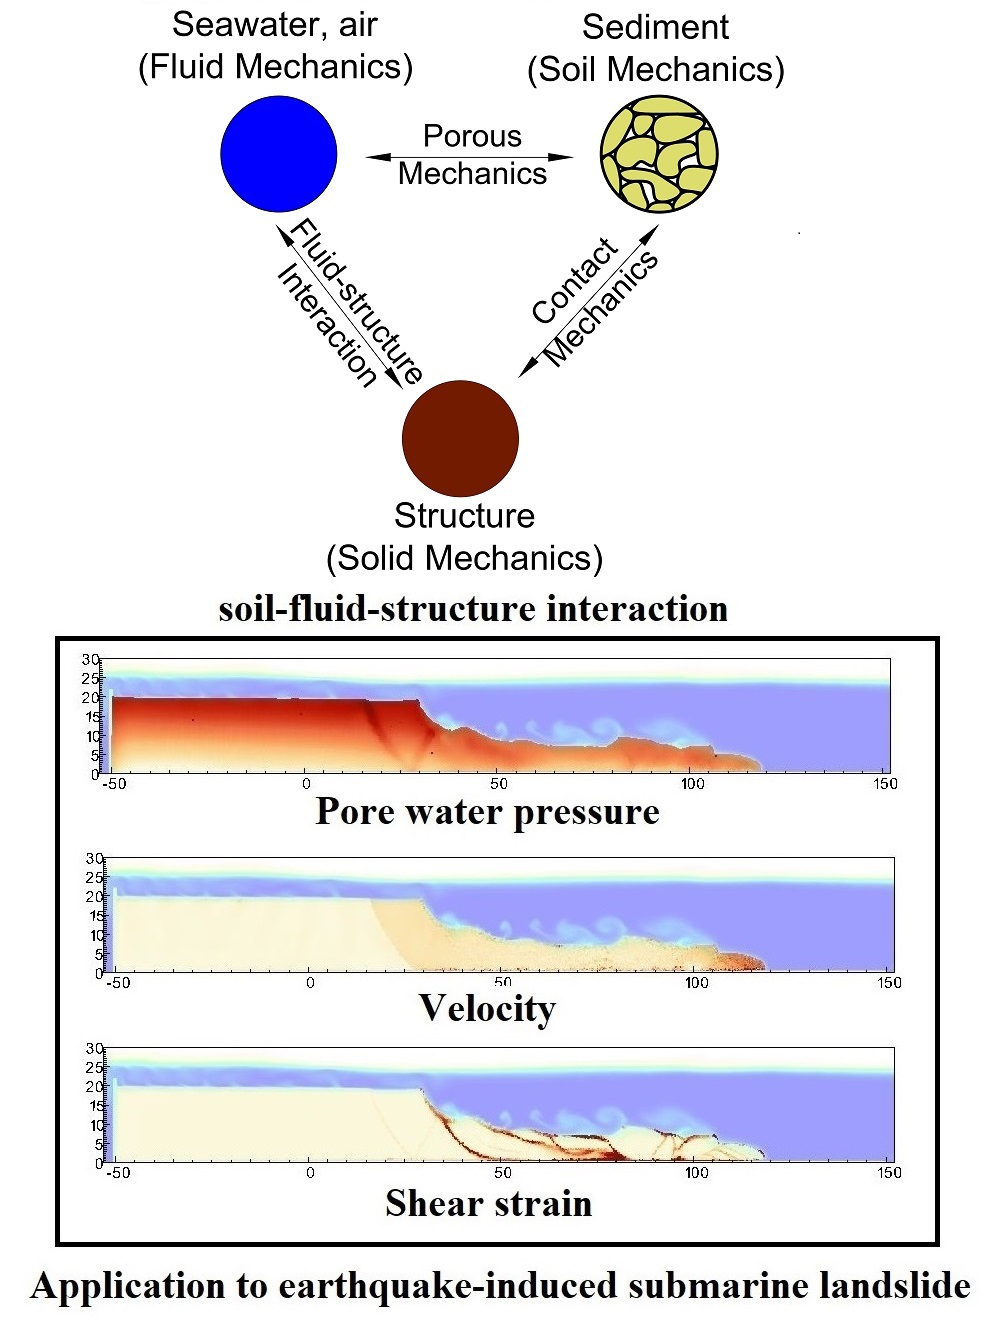
\includegraphics[scale=0.45]{abstract.jpg}
%
%
\end{graphicalabstract}

%%Research highlights
\begin{highlights}
\item MPMICE is introduced for multiphase flow in porous media.
\item Material Point method allows to model large deformation of non-isothermal porous media.
\item ICE (compressible multi-material CFD formulation) allows to stablize pore water pressure and turbulent flow.
\item MPMICE is validated and apply to simulate the earthquake-induced submarine landslide.
\end{highlights}

\begin{keyword}
%% keywords here, in the form: keyword \sep keyword

%% PACS codes here, in the form: \PACS code \sep code

%% MSC codes here, in the form: \MSC code \sep code
%% or \MSC[2008] code \sep code (2000 is the default)
Material Point Method 
\sep MPMICE
\sep submarine landslide.
\end{keyword}

\end{frontmatter}

%
%
%
%______________________________________________________________________
%   Table of Contents    
%______________________________________________________________________
\newpage
\setcounter{secnumdepth}{-2}
\tableofcontents
%% \linenumbers

%______________________________________________________________________
\newpage
%
%
\section{\textsf{Nomenclature}}
\begin{tabular}{lll}
\\
\pmb{General variables}\\
\underline{\textsf{Variable}} & \underline{\textsf{Dimensions}} & \underline{\textsf{Description} }\\
$V$      				&   $[L^3]$     & Representative volume\\
$n$      				&           	& Porosity\\
$\pmb{\sigma}$ 			&  $[M/L^2]$ 	& Total stress tensor\\
$\delt$       			&  $[t]$      	& Time increment\\
$\pmb{b}$ 			    &  $[L/t]$ 	    & Gravity acceleration\\
$c_v$                   &  $[L^2/t^2]$  & Constant volume specific heat\\
$f_{d}$ 		  	    &  $[ML//t^2]$ 	& Drag forces in momentum exchange term\\
$f^{int}$ 		  	    &  $[ML//t^2]$ 	& Internal forces\\
$f^{ext}$ 		  	    &  $[ML//t^2]$ 	& External forces\\
$q_{fs}$ 		  	    &  $[ML//t^2]$ 	& Heat exchange term\\
$S$ 		  	    	&            	& Shape function\\
$\nabla S$ 				&            	& Gradient of shape function\\
\pmb{Solid phase}\\
\underline{\textsf{Variable}} & \underline{\textsf{Dimensions}} & \underline{\textsf{Description} }\\
$m_s   $       			&  $[M]$      	& Solid mass\\
$\rho_s$				&	$[M/L^3]$  	& Solid density\\
$\phi_s$				     &	$-]$  	& Solid volume fraction\\
$\overline{\rho}_s$		&	$[M/L^3]$  	& Average Solid density\\
$\pmb{x}_s$   			&  	$[L]$    	& Solid Position vector\\
$\pmb{U}_s$   			&  	$[L/t]$    	& Solid Velocity vector\\
$\pmb{U}_s$   			&  	$[L/t]$    	& Solid Velocity gradient vector\\
$\pmb{a}_s$   			&  	$[L/t^2]$   & Solid Acceleration vector\\
$\pmb{\sigma}^\prime$ 	&  $[M/L^2]$ 	& Effective Stress tensor\\
$e_s$         			&  $[L^2/t^2]$  & Solid Internal energy \\   
$T_s$           		&  $[T]$      	& Solid Temperature\\
$\pmb{F}_s$     		&       	    & Solid Deformation gradient\\
$V_s$     				&  $[L^3]$      & Volume\\
\end{tabular}

\newpage
%
%
\begin{table}[h!]
\centering
\begin{tabular}{lll}
\\
\pmb{Fluid phase}\\
\underline{\textsf{Variable}} & \underline{\textsf{Dimensions}} & \underline{\textsf{Description} }\\
$m_f   $       			&  $[M]$      	& Fluid mass\\
$\rho_f$	    		            &   $[M/L^3]$  	& Fluid density\\
$\phi_f$				      &   $-]$  	& Fluid volume fraction\\
$\overline{\rho}_f$		&  $[M/L^3]$  	& Average Fluid density\\
$\pmb{U}_f$   			&  $[L/t]$    	& Fluid Velocity vector\\
$\pmb{\sigma}_f$ 		&  $[M/L^2]$ 	& Fluid stress tensor\\
$\Delta p_f$ 				&  $[M/L^2]$ 	& Fluid isotropic pressure\\
$\pmb{\tau}_f$ 			&  $[M/L^2]$ 	& Fluid shear stress tensor\\
$p_f$ 		  			&  $[M/L^2]$ 	& Isotropic pressure\\
$e_f$         			&  $[L^2/t^2]$  & Fluid Internal energy $(c_vT_f)$ of the material per unit mass \\   
$T_f$           		&  $[T]$      	& Fluid Temperature\\
$\upsilon_f$    		&  $[L^3/M]$  	& Fluid Specific volume $\frac{1}{\rho_f}$\\
$\alpha_f$    		    &  $[1/T]$  	& Thermal expansion\\
$\mu$    		    &  $[M/L^2 T]$  	& Fluid vicousity\\

\pmb{Superscript}\\
\underline{\textsf{Variable}} & \underline{\textsf{Dimensions}} & \underline{\textsf{Description} }\\
$n$           			&               &    Current time step\\
$L$           			&               &    Lagrangian values\\
$n+1$         			&               &    Next time step\\
\pmb{Subscript}\\
$c$           			&               &    Cell-centered quantity\\
$p$           			&               &    Particle quantity\\
$i$           			&               &    Node quantity\\
$FC$           			&             	&    Face-centered quantity\\
$L, R $       			&             	&    Left and Right cell faces\\
\end{tabular}
\caption{Nomenclature}
\label{table:1}
\end{table}


\newpage
%
%__________________________________________________
%% main text
\section{\textsf{Introduction}}
Submarine landslides can pose significant threats to the offshore infrastructures and the coastal communities. Submarine landslides have three stages: triggering, failure, and post-failure. Erosion or earthquakes can trigger slope failures in the first stage. Following the failure, sediments move quickly after the post-failure stage. As a submarine landslide is triggered, sediment behaves like solid (soil) materials and changes to fluid-like behavior after failure. This phase transition makes it challenge to simulate the submarine landslides.\\

Due to this phase transition, submarine landslide can be modeled by either the Computational Fluid Dynamics (CFD) or the particle-based methods. For simulating submarine slides, CFD methods solve governing equations in a full-Eulerian framework for single-phase flows \cite{CFD1, CFD2} and for multi-phase flows \cite{CFD3, CFD4} with interface capturing techniques. While CFD can handle complex flows (such as turbulent flows), it cannot account for the triggering mechanism of submarine landslides because it is not straightforwad to consider 'soil constitutive laws' of sediment materials in the Eulerian framework. In contrast, particle-based methods can overcome this problem by using the Lagrangian framework. These methods have been extensively used to simulate landslides, like Material Point Method (MPM) \cite{Tran2019}, Smooth Particle Hydro Dynamics \cite{Capone2010}, Particle Finite Element Method \cite{Zhang2019}, or Coupled Eulerian Lagrangian Method \cite{Dey2016}. For simplicity, these simulations adopt total stress analysis which neglects the pore pressure development which is the key factor triggering slope failures. \\

Recent developments in particle-based methods model the coupling of fluid flow in porous media by sets of Lagrangian particles. For the MPM family, it is the double-point MPM (\cite{Bandara2015, Tampubolon2017, Baumgarten2019}) where fluid particles and solid particles are overlapped in a single computational grid. Even if fluid flows are considered, particle-based methods have numerical instability in modeling the fluid flow, which requires additional numerical treatments such as the B-bar method \cite{Bandara2015}, null-space filter \cite{nullspace}, or least square approximation \cite{Zheng2021, CPLS}. Indeed, CFD is a more optimal option for complex fluid flows especially dealing with large distortions of continuum fluid media. Therefore, it could be ideal to combine the CFD with particle-based methods. More than 50 particle-based methods have been developed to solve large deformations of solids over the last two decades \cite{Chen2017}, but the MPM appears to be the best candidate for coupling with the CFD. Because MPM incorporates a stationary mesh during computation, just like CFD. As such, both MPM and CFD can be coupled naturally in a unified computational mesh.\\
%
%
\begin{figure}[h]
\center
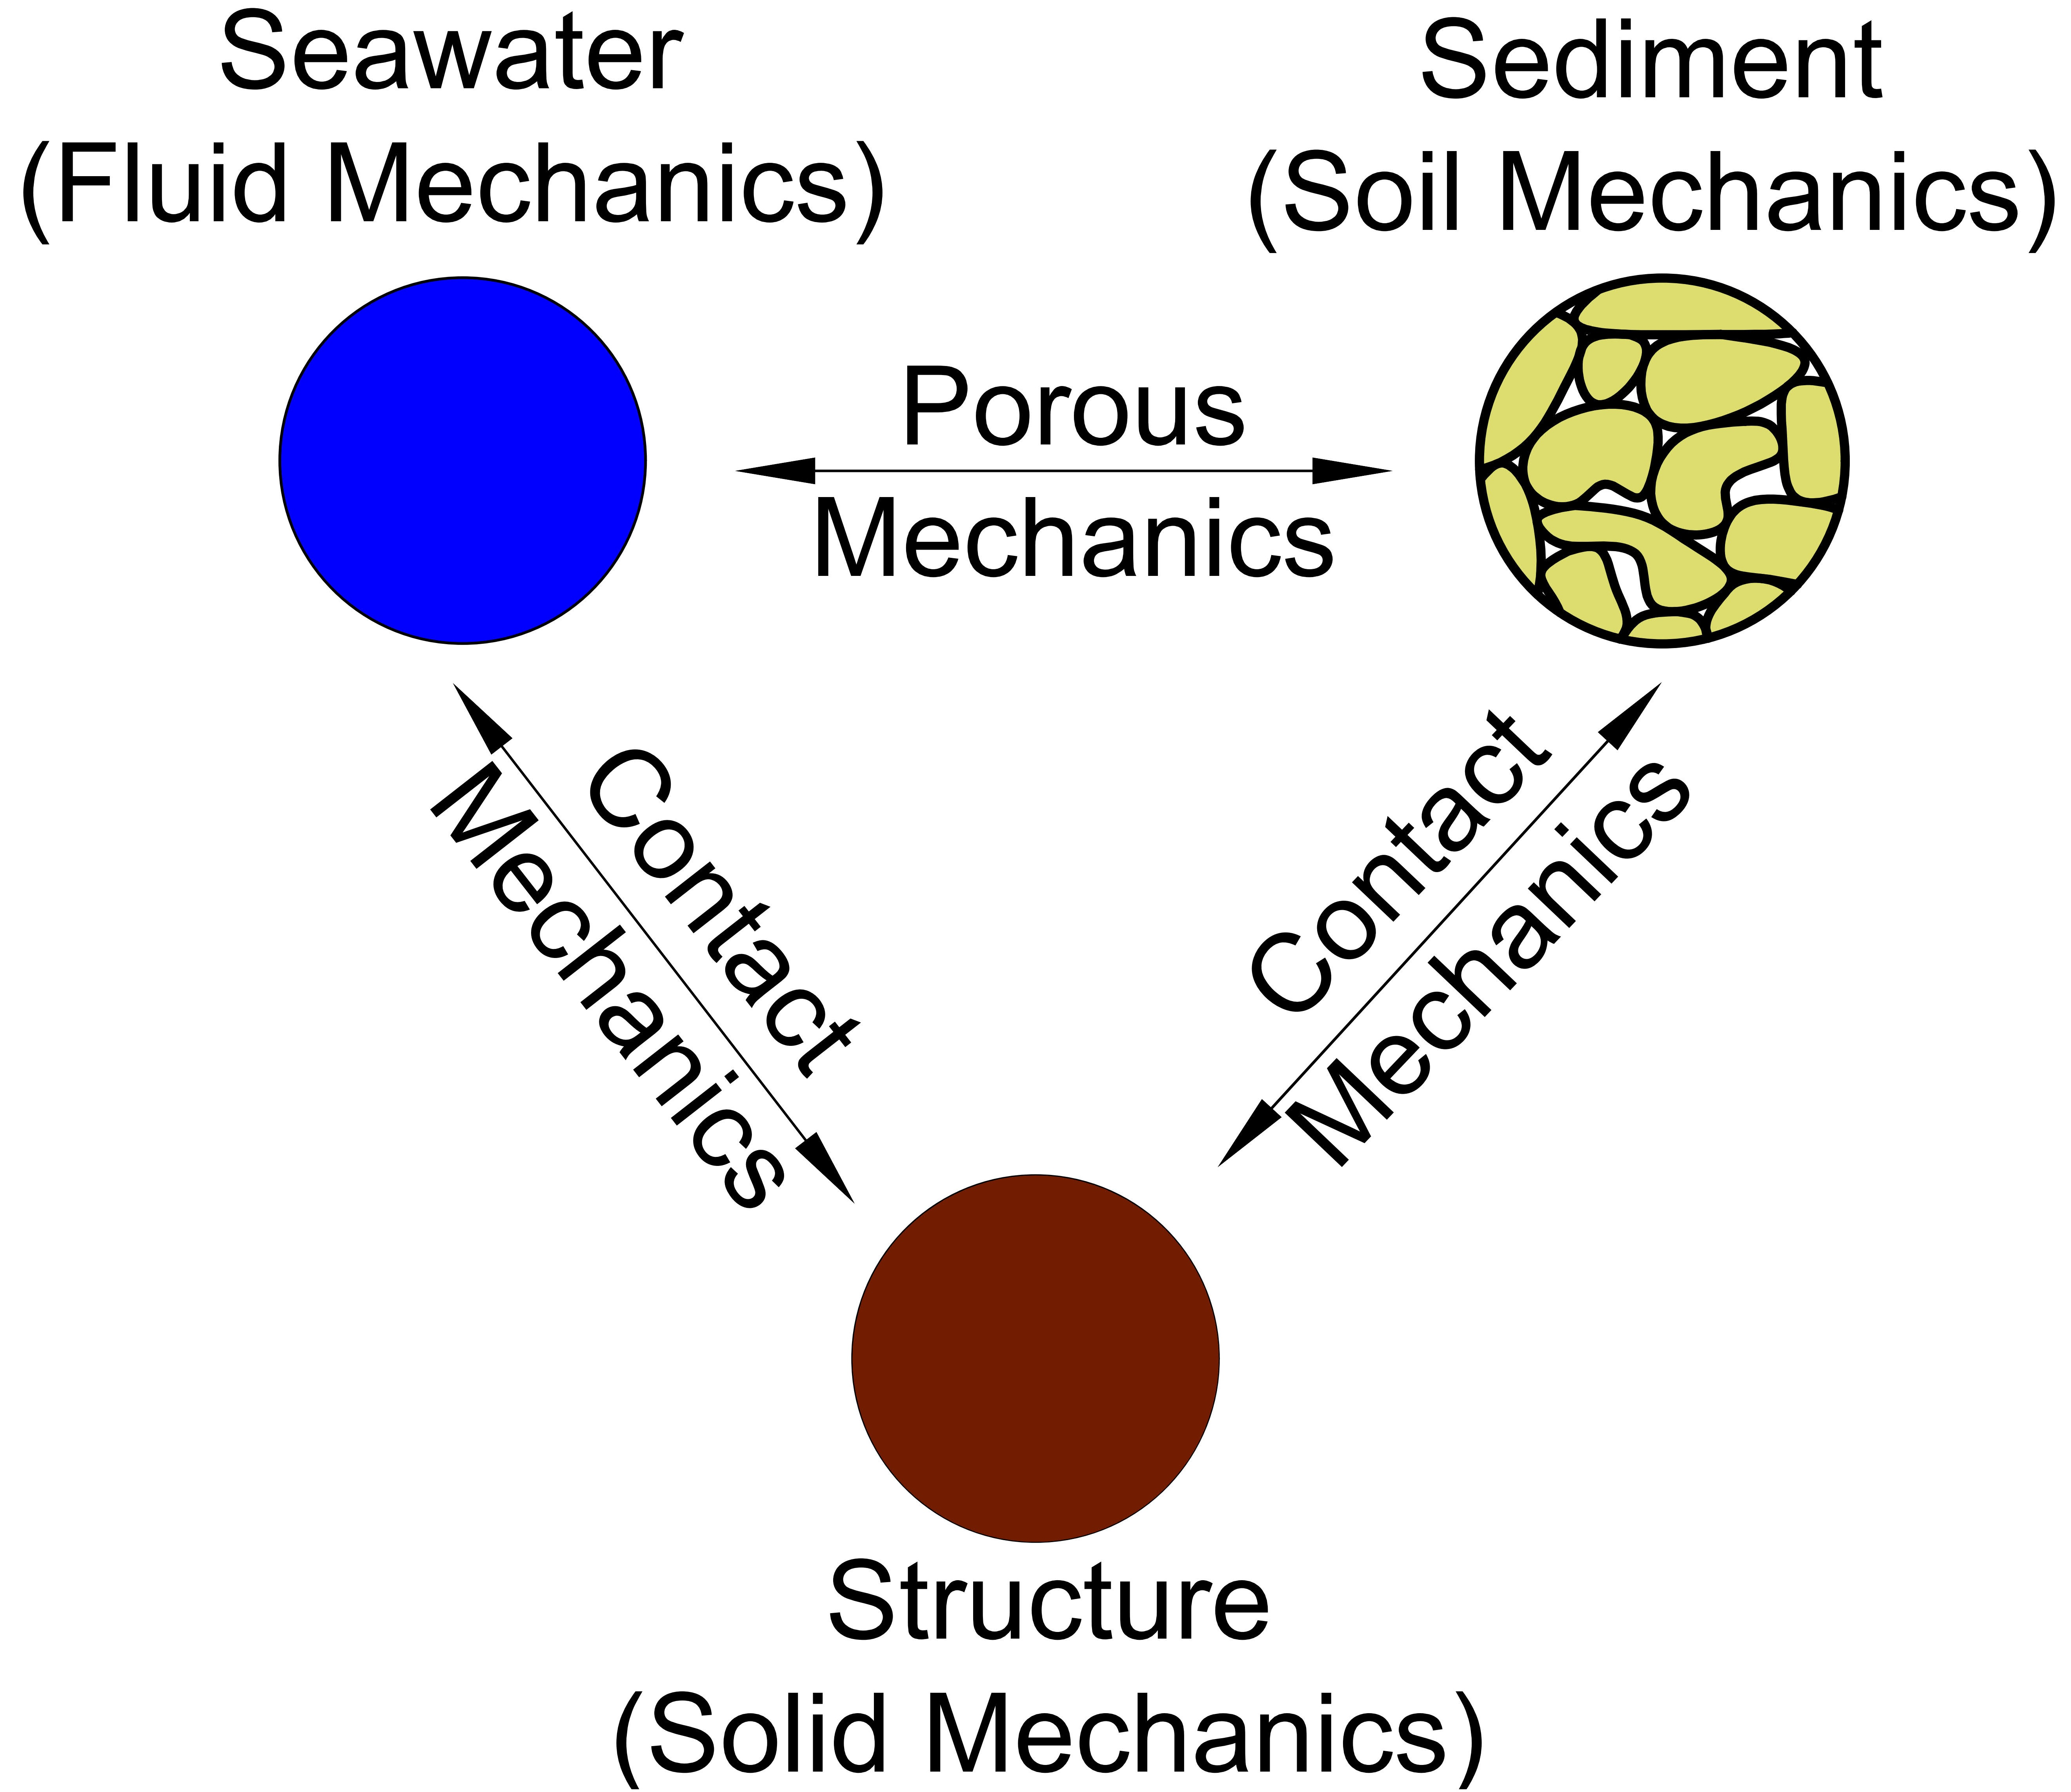
\includegraphics[scale=.3]{3phases.jpg}
\caption{Interaction between soil-fluid-structure}
\label{fig:3phases}
\end{figure}
%
%

%
%
\begin{figure}[h]
\center
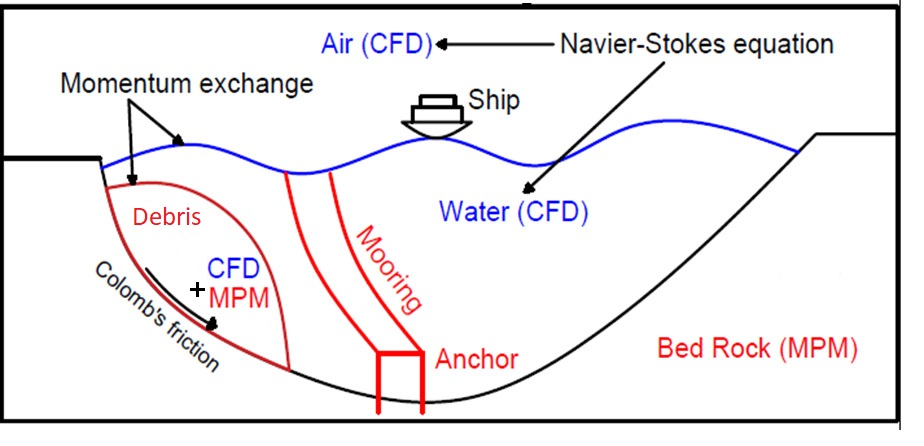
\includegraphics[scale=.4]{MPMICE.jpg}
\caption{Coupling of soil-water-structure interaction using MPMICE}
\label{fig:MPMICE}
\end{figure}
%
%

A numerical method for simulating soil-fluid-structure interaction (Figure \ref{fig:3phases}) involving large deformations, is presented in this work in order to simulate the interaction between sediment (soil), seawater (fluid) and offshore structures (structure) namely MPMICE (Figure \ref{fig:MPMICE}). In the MPMICE, the Material Point Method (MPM) is coupled with the Implicit Continuous Eulerian (ICE). The MPM method is a particle method that allows the porous soil to undergo arbitrary distortions. The ICE method, on the other hand, is a compressible, conservative finite volume technique with all state variables located at the cell center (temperature, velocity, mass, pressure). An initial technical report \cite{Kashiwa} at Los Alamos National Laboratory provided the theoretical and algorithmic foundation for the MPMICE, followed by the MPMICE development and implementation in the high-performance Uintah computational framework for simulating fluid-structure interactions \cite{MPMICE}. This paper primarily contributes futher to the development of the MPMICE for analyzing the \textbf{soil}-fluid-structure interaction, since sediment should be considered as a porous media (soil) and not as a solid to capture the evolution of the pore water pressure. Baumgarten et al. \cite{Baumgarten2021} made the first attempt at coupling the Finite Volume Method with the MPM for the simulation of soil-fluid interaction. Our contribution differs from the mentioned work in that we use the implicit time integration for the fluid phases instead of the explicit time integration.

%_______________________________
\section{\textsf{Theory and formulation}}
This section lay out the theoretical framework for the MPMICE model. We use the common notation of the continuum mechaniccs with vector and tensor denoted simply by using bold font and scalar denoted by using normal font. The notation
are shown in Table \ref{table:1}.
%_______________________________
\subsection{\textsf{Assumptions}}
The following assumptions are made for the MPMICE model.
\begin{enumerate}
\item Solid phases (MPM) are described in a Lagrangian formulation while fluid phases (ICE) are described in an Eulerian formulation in the framework of continuum mechanics and mixture theory.
\item Solid grains are incompressible while the fluid phase is compressible.
\item There is no mass exchange between solid and fluid phases.
\item Terzaghi's effective stress is valid. 
\end{enumerate}
%
%
%_______________________________
\subsection{\textsf{Governing equations}}
A representative element volume $\Omega$ is decomposed by two domains: solid domains $\Omega_s$ and fluid domains $\Omega_f$. Then, all domains are homogenized into two overlapping continua. Considering the volume fraction of solid $\phi_s = \Omega_s/\Omega$ and fluid $\phi_f = \Omega_f/\Omega$ with the true (or Eulerian) porosity $n=\sum{\phi_f}$ of the representative element volume, the average density of solid and fluid phases are defined as:\\
%
%
\begin{equation}
    \label{density} 
  \overline{\rho}_s   = \phi_s \rho_s, \qquad  \overline{\rho}_f   = \phi_f \rho_f \quad
\end{equation}
%
%
The mass of solid and fluid phase are:\\
%
%
\begin{equation}
    \label{mass} 
  m_s   = \int_{\Omega} \rho_s dV = \overline{\rho}_s V, \qquad  m_f   = \int_{\Omega} \rho_f dV = \overline{\rho}_f V
\end{equation}
%
%
Reviewing the Terzaghi's effective stress concept for the saturated porous media, the total stress $\pmb{\sigma}$ is calculated by:\\
%
%
\begin{equation}
    \label{Terzaghi} 
  \pmb{\sigma}   = \pmb{\sigma}^\prime -p_f\pmb{I}
\end{equation}
%
%
The balance equations are derived based on the mixture theory. The average thermodynamic state of the fluid phases are given by the vector $[m_f,\pmb{U}_f,e_f,T_f,\upsilon_f]$ which are mass, velocity, internal energy, temperature, specific volume. The average state of the solid phases are given by the vector $[m_s,\pmb{U}_s,e_s,T_s,\pmb{\sigma}^\prime]$ which are mass, velocity, internal energy, temperature, effective stress. Here, we summarize the final form of the equations while the derivation is presented in detail in the Appendix. \\
%
%_______________________________
% mass
%_______________________________
\underline{\hspace{5in}}\\
\underline{\textsf{Mass Conservation}}\\
The mass balance equations for both fluid and solid phases are:\\
%
%
\begin{equation}
    \label{massbalance}
   \frac{1}{V}\frac{D_fm_f}{Dt} = 0, \\ 
   \frac{1}{V}\frac{D_sm_s}{Dt} = 0    
\end{equation}
%
%_______________________________
% momentum
%_______________________________
\underline{\hspace{5in}}\\
\underline{\textsf{Momentum Conservation}}\\
The momentum balance equation for the fluid phase is:\\
%
%
\begin{equation}
     \frac{1}{V}\frac{D_f(m_f \pmb{U}_f)}{Dt} = -n\nabla P_{eq} +  \nabla \cdot \pmb{\tau}_f + \overline{\rho}_f \pmb{b} +
     \pmb{f}_{d}
\end{equation}
%
%
The momentum balance equation for the solid phase is:\\
%
%
\begin{equation}
     \frac{1}{V}\frac{D_s(m_s \pmb{U}_s)}{Dt} = 
    \nabla \cdot (\pmb{\sigma}^\prime) - (1-n) \nabla p_f 
    + \overline{\rho}_s \pmb{b}
    - \pmb{f}_{d}
\end{equation}
%
%
%_______________________________
% Energy
%_______________________________
\underline{\hspace{5in}}\\
\underline{\textsf{Energy Conservation}}\\
The internal energy balance equation for the fluid phase is:
%
%
\begin{equation}
    \label{fluidenergy}
     \frac{1}{V}\frac{D_f(m_f e_f)}{Dt} = 
    -\overline{\rho}_f P_{eq}  \frac{D_f\upsilon_f}{Dt} + \pmb{\tau}_f : \nabla \pmb{U}_f + \nabla \cdot \pmb{q}_f + q_{sf}
\end{equation}
%
%
The internal energy balance equation for the solid phase is:
%
%
\begin{equation}
    \label{solidenergy}
     \frac{1}{V}\frac{D_s(m_s e_s)}{Dt} = \pmb{\sigma}^\prime:\nabla \pmb{U}_s + \nabla \cdot \pmb{q}_s - q_{sf} 
\end{equation}
%
%
\underline{\hspace{5in}}\\
To close the systems of the equations, it requires the additional models: \\
(1) Exchange momentum model (computing drag force $\pmb{f}_{d}$). \\
(2) Energy exchange model (computing temerature exhange term $q_{sf}$). \\
(3) Optional turbulent model to compute the viscous shear stress $\pmb{\tau}_f$.\\
(4) A constitutive equation to describe the stress - strain behaviour of solid phase (computing effective stress $\pmb{\sigma}^\prime$). \\
(5) An equation of state to establish relations between thermodynamics variables of each fluid materials $[P_{eq}, \overline{\rho}_f, \upsilon_f, T_f, e_f]$. \\
Here, $P_{eq}$ is "equilibrium" pressure which is defined as pressure enables mass of fluid material to fills in an entire porosity volume with no ongoing compression or expansion with given true density $\rho_f$ and temperature $T_f$.  Four thermodynamic relations for the equation of states are:
%
%
\begin{equation}
\begin{gathered}
  e_f =  e_f (T_f, \upsilon_f)\\
 \upsilon_f =  \upsilon_f (T_f, P_{eq})\\
  \phi_f = \upsilon_f \overline{\rho}_f\\
  0 = n - \sum_{f=1}^{N_f} \upsilon_f \overline{\rho}_f\\
\end{gathered}
\end{equation}
%
%
Solving the equation of state (see Appendix's section 'Evolution of specific volume') leading to the rate of the equilibrium pressure of fluid mixture as:
%
%
\begin{equation}
\sum_{f=1}^{N_f} \phi_f \kappa_f \frac{D_f P_{eq}}{Dt} = - \nabla \cdot \pmb{U} + \sum_{f=1}^{N_f} \phi_f \alpha_f \frac{D_f T_f}{Dt}
\end{equation}
%
%
where $\pmb{U} = \nabla \cdot (\sum_{s=1}^{N_s} \phi_s \pmb{U}_s + \sum_{f=1}^{N_f}  \phi_f \pmb{U}_f)$.
And the rate of the specific volumne of fluid materias are:
%
%
\begin{equation}
\label{specific volume}
\overline{\rho}_f \frac{D_f \upsilon_f }{Dt} = f_f^{\phi} \nabla \cdot \pmb{U} + (\phi_f \alpha_f \frac{D_f T_f}{Dt} - f_f^{\phi} \sum_{n=1}^{N} \phi_n \alpha_n \frac{D_n T_n}{Dt})
\end{equation}
where $ f_f^{\phi} = (\phi_f  \kappa_f ) / (\sum_{n=1}^{N} \phi_n \kappa_n)$ with  $\kappa_f$ being f-material bulk compressibility and $\alpha$ is the constant pressure thermal expansitivity of fluids.
%
%
%_______________________________
\subsubsection{Equation of state for fluid plases}
%
%
\begin{figure}[h]
\center
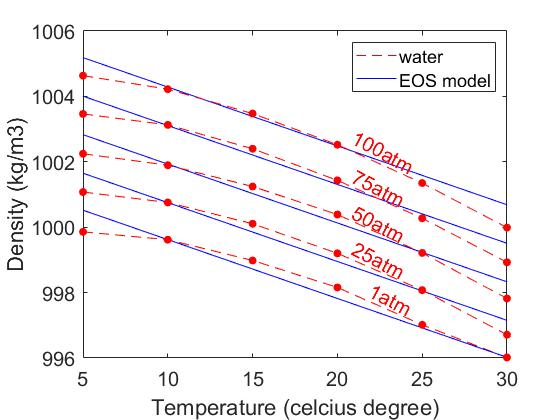
\includegraphics[scale=.5]{water1.jpg}
\caption{Equation of state of water}
\label{fig:water1}
\end{figure}
%
%
The equation of state establishes relations between thermodynamics variables $[P_f, \rho_f, T_f]$. The choice of the equation of state depends on the types of the fluid materials. For example, for the air, it is possible to assume the equation of state for the perfect gas which obeys:
%
%
\begin{equation}
    P_f = \rho_f R T_f
\end{equation}
%
%
where $R$ is the gas constant. For the water, a simple linear equation of state is in the following form:
%
%
\begin{equation}
    P_f = P_{ref} + K_f (\rho_f - \rho_ref - \alpha_f(T_f - T_{ref}))
\label{waterEOS}
\end{equation}
%
%
where reference pressure $P_{ref}$ = 1 atm = 101325 Pa, reference temperature $T_{ref}$ = 10°C, reference density  $\rho_{ref}$ = 999.8 kg/m3, the bulk modulus of water $K_f$ = 2 GPa, and the water thermal expansion $\alpha_f$ = 0.18 kg/m3 per Celsius degree. Equation (\ref{waterEOS}) matches well with the state of the water (see Figure \ref{fig:water1}).
%_______________________________
\subsubsection{Constitutive soil model}
As a result of the explicit MPM formulation, we can derive the constitutive law in the updated Lagrangian framework of "small strain - large deformation". Therefore, the rotation of the particles (representative element volume) is manipulated by rotating the Cauchy stress tensor. First, the deformation gradient is decomposed into the polar rotation tensor $\pmb{R}_s^{n+1}$ and sketch tensor $\pmb{V}_s^{n+1}$ as
%
%
\begin{equation}
     \pmb{F}_s^{n+1} = \pmb{V}_s^{n+1} \pmb{R}_s^{n+1}
\end{equation}
%
%
Then, before calling the constitutive model, the stress and strain rate tensor are rotated to the reference configuration as
%
%
\begin{equation}
     \pmb{\sigma}^{\prime,n*} =  (\pmb{R}_s^{n+1})^T \pmb{\sigma}^{\prime,n*} \pmb{R}_s^{n+1}
\end{equation}
%
%
\begin{equation}
    \delta \pmb{\epsilon}^{n*} =  (\pmb{R}_s^{n+1})^T \delta \pmb{\epsilon}_s^{n*} \pmb{R}_s^{n+1}
\end{equation}
%
%
Using the constitutive model with the input tensors $\pmb{\sigma}^{\prime,n*}, \delta \pmb{\epsilon}^{n*}$ to compute the Cauchy stress tensor at the advanced time step $\pmb{\sigma}^{\prime,n+1*}$ then rotating it back to current configuration
%
%
\begin{equation}
    \pmb{\sigma}^{\prime,n+1} =  \pmb{R}_s^{n+1} \pmb{\sigma}^{\prime,n+1*} (\pmb{R}_s^{n+1})^T
\end{equation}
%
%
In this paper, we adopt the hyper-elastic Neo Hooken model for the structure materials and additionally Mohr-Coulomb failure criteria for the soil (porous media) materials. The Cauchy stress of the hyper-elastic Neo Hookean model can be written as:
%
%
\begin{equation}
    \pmb{\sigma}^{\prime} =  \frac{ \lambda ln(J)}{J} + \frac{\mu}{J} (\pmb{F} \pmb{F}^T - \pmb{J})
\end{equation}
%
%
where $\lambda$ and $\mu$ are bulk and shear modulus ad J is the determinant of the deformation gradient $\pmb{F}$. And the yield function f and flow potentials g of the Mohr-Coulomb can be written as:
%
%
\begin{equation}
\begin{gathered}
   f =  \sigma_1^{\prime} -  \sigma_3^{\prime} -2c^{\prime} cos(\phi^{\prime}) - (\sigma_1^{\prime} +  \sigma_3^{\prime})sin(\phi^{\prime})\\
   g =  \sigma_1^{\prime} -  \sigma_3^{\prime} -2c^{\prime} cos(\psi^{\prime}) - (\sigma_1^{\prime} +  \sigma_3^{\prime})sin(\psi^{\prime})
\end{gathered}
\end{equation}
%
%
where the $c^{\prime}$, $\phi^{\prime}$ and $\psi^{\prime}$ are cohesion and friction angle and dilation angle. $\sigma_1^{\prime}$ and $\sigma_3^{\prime}$ are maximum and minimum principal stress.
%_______________________________
\subsubsection{Momentum and Energy exchange model}
Currently, the energy exchange coefficient $H_{sf}$ is assumed to be constant for the sake of simplicity. Then the energy exchange can be written as:
%
%
\begin{equation}
     q_{sf} = H_{sf} \phi_f \phi_s (T_f -T_s)
\end{equation}
%
%
For the momentum exchange, we assume that the drag force $\pmb{f}_{d}$ depends on the average grain size of the grains $D_p$, the porosity $n$, the fluid vicosity $\mu_f$, and is propotional to the relative velocities of soil grains and fluid $(\pmb{U}_s - \pmb{U}_f)$. Based on recent investigation of CFD simulations of fluid flow around mono- and bi-disperse packing of spheres for $0.1 < \phi_s < 0.6$ and $Re < 1000$ \cite{Drag}. The drag force is given by: \\
%
%
\begin{equation}
     \pmb{f}_{d} = \frac{18\phi_s(1-\phi_s)\mu_f}{D_p^2} F(\phi_s, Re) (\pmb{U}_s - \pmb{U}_f)  
\label{fd}
\end{equation}
%
%
where Reynolds number $Re$ are computed as:
%
%
\begin{equation}
     Re = \frac{n \rho_f D_p}{\mu_f} |\big\|(\pmb{U}_s - \pmb{U}_f)\big\|
\end{equation}
%
%
The function $F(\phi_s, Re)$ can be calculated as:
%
%
\begin{equation}
     F(\phi_s, Re)  = F(\phi_s, 0)  + \frac{0.413Re}{24 (1-\phi_s)^2} (\frac{(1-\phi_s)^{-1}+3\phi_s(1-\phi_s)+8.4Re^{-0.343}}{1+10^{3\phi_s}Re^{-(1+4\phi_s)/2}})
\end{equation}
%
%
where the low Reynold coefficient $ F(\phi_s, Re\rightarrow0)$ is:
%
%
\begin{equation}
     F(\phi_s, 0)  = \frac{10\phi_s}{ (1-\phi_s)^2}+(1-\phi_s)^2(1+1.5\sqrt{\phi_s})
\end{equation}
%
%
When validating the model with analytical solution, it requires to know the hydraulic conductivity. In such case, we convert the equation (\ref{fd}) to Kozeny-Carman formula by assuming $F(\phi_s, Re) = 10\phi_s/(1-\phi_s)^2$, then the hydraulic conductivity will be expressed as  $K = D_p^2 (1-\phi_s)^3 / 180 \mu \phi_s^2$.

\subsubsection{Solving momentum exchange with an implicit solve}
The derivation of the implicit integration for the momentum exchange is presented in the Appendix's section 'Momentum exchange with an implicit solve'. The linear equations 
has the form:
%
\[ \begin{vmatrix} (1 + \beta_{12})  &  -\beta_{12} \\
                  -\beta_{21}       &  (1 + \beta_{21})
    \end{vmatrix}
    \begin{vmatrix} \Delta \pmb{U}_{f} \\
                    \Delta \pmb{U}_{s}
    \end{vmatrix}
    =
    \begin{vmatrix}  \beta_{12}(\pmb{U}_{s}^{*} - \pmb{U}_{f}^{*}) \\
                    \beta_{21}(\pmb{U}_{f}^{*} - \pmb{U}_{s}^{*})
    \end{vmatrix}                
\]
%
%
where the intermediate velocity can be calculated by
%
\begin{equation}
\begin{gathered}
\pmb{U}_{f}^{*} = \pmb{U}_{f}^{n} + \delt (-\frac{\nabla P_{f}^{n+1}}{\rho_f^n}  + \frac {\nabla \cdot \pmb{\tau}_f^{n}}{\overline{\rho}^n_{f}} + \pmb{b}) \\
\pmb{U}_{s}^{*} = \pmb{U}_{s}^{n} + \delt (\frac{\nabla \cdot \pmb{\sigma}^{'n}}{\overline{\rho}^n_{s}}    - \frac{\nabla P_{f}^{n+1}}{\rho_s}  + \pmb{b})
\end{gathered}
\end{equation}
%
%
Also, the momentum exchange coefficient can be computed at every time step as $\beta_{12} = K/\overline{\rho}_{f}^n$ and $\beta_{21} = K/\overline{\rho}_{s}^n$ with the coefficient $K =  18\phi_s(1-\phi_s)\mu_f  F(\phi_s, Re) /D_p^2$.

%_______________________________
\subsubsection{Turbulent model}
The turbulent effect is modelled using a statistical approach namely large-eddy simulation. In this approach, the micro-scale turbulent influence in the dynamics of the macro-scale motion is computed through simple models like Smagorinsky model. In the Smagorinsky mode, the residual stress tensor is:
%
\begin{equation}
     \tau_{ij} = 2 \mu_{eff} (\overline{S}_{ij} - \frac{1}{3} \delta_{ij} \overline{S}_{kk}) + \frac{1}{3} \delta_{ij} \tau_{kk}
\end{equation}
%
%
where the the strain rate tensor is given by
%
\begin{equation}
     \overline{S}_{ij} = \frac{1}{2} (\frac{\delta \overline{\pmb{U}}_i}{\delta x_j} + \frac{\delta \overline{\pmb{U}}_j}{\delta x_i})
\end{equation}
%
%
and the effective viscosity is sum of molecular viscosity and turbulent viscosity $\mu_{eff} = \mu + \mu_t$ in which the turbulent viscosity $\mu_t$ is calculated by
%
\begin{equation}
    \mu_t = (C_s \triangle)^2 \sqrt{2 \overline{S}_{ij} \overline{S}_{ij}}
\end{equation}
%
%
where $C_s$ is the Smagorinsky constant and $\triangle = \sqrt[3]{dx dy dz}$ is the grid size that defines the subgrid length scale. 
%
%_______________________________
\section{\textsf{Numerical implementation}}
\label{Discretization}
The fluid phase is discretized in the grid with the state variables stored at the centroid of the cells $[\rho_{fc},\pmb{U}_{fc},T_{fc},\upsilon_{fc}]$ while the solid phase is discretized in the particles with the state variables $[m_{sp},\pmb{U}_{sp},T_{sp},\pmb{\sigma}^\prime_{sp}]$. The time discretization are solved using the following steps:\\
%
%
\subsection{\textsf{Interpolation from Solid Particle to Grid}}
%
%
The nodal values of the solid state (mass, velocity, temperature, volume) are:
%
%
\begin{equation}
\begin{gathered}
     m_{si}^n = \sum{S_{ip}m_{sp}}\\
     \pmb{U}_{si}^n = \frac {\sum{S_{ip} (m\pmb{U})_{sp}^n}}{m_{si}^n}\\
     T_{si}^n = \frac {\sum{S_{ip} (mT)_{sp}^n}}{m_{si}^n}\\
     V_{si}^n = \frac {\sum{S_{ip} (mV)_{sp}^n}}{m_{si}^n}\\
     \pmb{\sigma}_{si}^n = \frac {\sum{S_{ip} (\pmb{\sigma}V)_{sp}^n}}{V_{si}^n}\\
\end{gathered}
\end{equation}
%
%
The nodal internal forces is calculated by
%
%
\begin{equation}
     \pmb{f}_{si}^{int,n} = -\sum{\nabla S_{ip} (\sigma_{sp}^\prime)^n V_{sp}^n}
\end{equation}
%
%
The nodal external forces $f_{si}^{ext,n}$ and extra momentum from contact forces are computed here. The nodal velocity and nodal temperature are applied boundary conditions.\\
Then we compute the solid cell variables as:
%
%
\begin{equation}
\begin{gathered}
     m_{sc}^n = \sum{S_{ci}m_{si}}\\
   \rho_{sc}^n = \frac{m_{sc}^n}{V}\\  
     \pmb{U}_{sc}^n = \sum{S_{ci} \pmb{U}_{si}^n}\\
     T_{sc}^n = \sum{S_{ci} T_{si}^n}\\
     V_{sc}^n = \sum{S_{ci} V_{si}^n}\\
     \pmb{\sigma}_{sc}^n = \sum{S_{ci} \pmb{\sigma}_{si}^n}\\
\end{gathered}
\end{equation}
%
%
\subsection{\textsf{Compute equation of state for fluid phase}}
Considering the total fluid materal volume of a cell is:
%
%
\begin{equation}
\label{V}
    V_{total} = \sum_{f=1}^{N_f} M_f \upsilon_f 
\end{equation}
%
%
Then we need to find $P_{eq}$ which allows each fluid materials obey their equation of states $[P_f, \rho_f, \upsilon_f, T_f, e_f]$ but also allow mass of all fluid materials to fill the entire the pore volume without ongoing compression or expansion following the condition:
%
%
\begin{equation}
    0 = n - \sum_{f=1}^{N_f} \upsilon_f \rho_f\\
\label{n}
\end{equation}
%
%
Then, we can use he Newton-Raphson interation to find the value of $P_{eq}$ which satisfies the equation (\ref{V}, \ref{n}) and each equation of states of each fluid materials.
\subsection{\textsf{Compute faced-centered velocity}}
Following the derivation in the Appendix: Advanced Fluid Pressure, we first compute the fluid face-centered velocity as\\
%
%
\begin{equation}
\label{faced_vel_fluid}
    \pmb{U}_{f,FC}^{*} = \frac{(\overline{\rho} \pmb{U})_{f,FC}^n}{\overline{\rho}_{f,FC}^n} + \delt (-\frac{\nabla^{FC} P_{eq}}{\rho_{f,FC}^n}  +\frac{\nabla^{FC} \cdot \pmb{\tau}^{n}}{\overline{\rho}_{s,FC}}+ \pmb{b})
\end{equation}
%
%
The equation (\ref{faced_vel_fluid}) is discretized in three dimension (noted that $\nabla^{FC} \cdot \pmb{\tau} = 0$), for example the discretized equation in the x direction is
%
\begin{equation}
U_{fx}^{*} = \frac{(\overline{\rho} U)_{fx,R}^n + (\overline{\rho} U)_{fx,L}^n}{\overline{\rho}_{fx,L}^n + \overline{\rho}_{fx,R}^n} + \delt (-\frac{2(\upsilon_{fx,L}^n \upsilon_{fx,R}^n)}{\upsilon_{fx,L}^n + \upsilon_{fx,R}^n} \frac{P_{eqx,R} - P_{eqx,L}}{\Delta x} + b_x)
\end{equation}
%
%
The face-centered solid velocity can be calculated as
\begin{equation}
\label{faced_vel_solid}
\pmb{U}_{s,FC}^{*} = \frac{(\overline{\rho} \pmb{U})_{s,FC}^n}{\overline{\rho}_{s,FC}^n} + \delt ( \frac{\nabla^{FC} \cdot \pmb{\sigma}_c^{'n}}{\overline{\rho}_{s,FC}}    - \frac{\nabla^{FC} P_{eq}}{\rho_s}   + \pmb{b})
\end{equation}
The equation (\ref{faced_vel_solid}) is discretized in three dimension(noted that $\nabla^{FC} \cdot \sigma_{ij} = 0$ with $i \neq j$), for example the discretized equation in the x direction is
%
\begin{equation}
U_{sx}^{*} = \frac{(\overline{\rho} U)_{sx,R}^n + (\overline{\rho} U)_{sx,L}^n}{\overline{\rho}_{sx,L}^n + \overline{\rho}_{sx,R}^n} + \delt (\frac{2(\sigma_{xx,R} - \sigma_{xx,L})}{(\overline{\rho}_{sx,L}^n + \overline{\rho}_{sx,R}^n)\Delta x}-\frac{P_{eqx,R} - P_{eqx,L}}{\rho_s \Delta x} + b_x)
\end{equation}
%
%
Computing the modified faced-centered velocity $\pmb{U}_{FC}^{L}$ considering the momentum exchange
%
\begin{equation}
\begin{gathered}
   \pmb{U}_{f,FC}^{L} = \pmb{U}_{f,FC}^{*} + \Delta \pmb{U}_{f,FC}\\
   \pmb{U}_{s,FC}^{L} = \pmb{U}_{s,FC}^{*} + \Delta \pmb{U}_{s,FC}
\end{gathered}
\end{equation}
%
%
By solving the linear equation below to obtain the increment of velocity
%
\[ \begin{vmatrix} (1 + \beta_{12,FC})  &  -\beta_{12,FC} \\
                  -\beta_{21,FC}       &  (1 + \beta_{21,FC})
    \end{vmatrix}
    \begin{vmatrix} \Delta \pmb{U}_{f,FC} \\
                    \Delta \pmb{U}_{s,FC}
    \end{vmatrix}
    =
    \begin{vmatrix}  \beta_{12,FC}(\pmb{U}_{s,FC}^{*} - \pmb{U}_{f,FC}^{*}) \\
                    \beta_{21,FC}(\pmb{U}_{f,FC}^{*} - \pmb{U}_{s,FC}^{*})
    \end{vmatrix}                
\]
%
%
\subsection{\textsf{Compute advanced fluid pressure (implicit scheme)}}
We solve the generalized Poisson's equation below by employing a preconditioned conjugate gradient technique with a multi-grid pre-conditioner
%
\begin{equation}
  \left(  
   \kappa - \nabla^c \frac{\delt}{\overline{\rho}_{f,FC}} \cdot \nabla^{FC}
  \right) \Delta P_c^{n}
  = - \nabla^c \cdot \pmb{U}_{f,FC}^{L}
\end{equation}
%
%
The advanced fluid pressure at cell center is
%
\begin{equation}
  P_c^{n+1} = P_{eq} + \Delta P_c^{n}
\end{equation}
%
%
Finally, the faced-centered advanced fluid pressure is
%
%
\begin{equation}
    P_{f,FC}^{n+1} = (\frac{P_{f,L}^{n+1}}{\overline{\rho}_{f,L}^n} + \frac{P_{f,R}^{n+1}}{\overline{\rho}_{f,R}^n}) / (\frac{1}{\overline{\rho}_{f,L}^n} + \frac{1}{\overline{\rho}_{f,R}^n}) = (\frac{P_{f,L}^{n+1} \overline{\rho}_{f,R}^n + P_{f,R}^{n+1} \overline{\rho}_{f,L}^n}{\overline{\rho}_{f,L}^n \overline{\rho}_{f,R}^n})
\end{equation}
%
%
\subsection{\textsf{Compute viscous shear stress term of the fluid phase}}
This part compute the viscous shear stress $\Delta (m \pmb{U})_{_{fc},\tau}$ for a single vicous compressible Newtonian fluid and optionally shear stress induced by the turbulent model.
%
%
\subsection{\textsf{Compute nodal internal temperature of the solid phase}}
%
%
The nodal internal temperature rate is computed based on the heat conduction model
%
%
\begin{equation}
     dT_{si}^L = \frac{(\Delta W_{si}^n + \nabla^i \cdot \pmb{q}_{si}^n)}{m_{si}^n}
\end{equation}
%
%
where $\Delta W_{si}^n = \pmb{\sigma}^\prime : \nabla \pmb{U}_s$ is the mechanical work rate computed from the constitutive model. The nodal internal temperature is calculated by
\begin{equation}
     T_{si}^L = T_{si}^n + dT_{si}^L
\end{equation}
%
%
\subsection{\textsf{Compute and integrate acceleration of the solid phase}}
After interpolating from material points to the nodes, the nodal acceleration and velocity are calculate by
%
%
\begin{equation}
     \pmb{a}_{si}^{L-} = \frac{\pmb{f}_{si}^{int,n} + \pmb{f}_{si}^{ext,n}}{m_{si}^n} + \pmb{g}
\end{equation}
\begin{equation}
     \pmb{U}_{si}^{L-} = \pmb{U}_{si}^n + \pmb{a}_{si}^{L-} \delt
\end{equation}
%
%
\subsection{\textsf{Compute Lagrangian value (mass, momentum and energy)}}
For the fluid phase, the linear momentum rate, the energy rate are
\begin{equation}
 \Delta (m \pmb{U})_{fc} = V n_c^n \nabla^c P_{fc}^{n+1} +\Delta (m \pmb{U})_{_{fc},\tau} + V \overline{\rho}_{fc}^n g
\end{equation}
%
%
\begin{equation}
 \Delta (me)_{fc} = V n_c^n P_{fc}^{n+1} \nabla^c \cdot \pmb{U}_{f,FC}^{*} + \nabla^c \cdot \pmb{q}_{fc}^n
\end{equation}
%
%
The Lagrangian value of the mass, linear momentum and energy of fluid phase without momentum exchange are
%
%
\begin{equation}
 m_{fc}^L = V \overline{\rho}_{fc}^n 
\end{equation}
%
%
\begin{equation}
 (m \pmb{U})_{fc}^{L-} = V \overline{\rho}_{fc}^n \pmb{U}_{fc}^n + \Delta (m \pmb{U})_{fc} 
\end{equation}
%
%
\begin{equation}
 (me)_{fc}^{L-} = V \overline{\rho}_{fc}^n T_{fc}^n    c_v + \Delta (me)_{fc} 
\end{equation}
%
%
For the solid phase, the Lagrangian value of the linear momentum and energy of solid phase are
%
\begin{equation}
 m_{sc}^L = m_{sc}^n
\end{equation}
%
\begin{equation}
 (m \pmb{U})_{sc}^{L-} = \sum{S_{ci} m_{si}^n \pmb{U}_{si}^{L-}} + V (1-n_c^n) \nabla^c P_{fc}^{n+1}
\end{equation}
%
\begin{equation}
 (me)_{sc}^{L-} =  \sum{S_{ci} m_{si}^n T_{si}^L}
\end{equation}
%
%
To consider the momentum exchange, the Lagrangian velocity is modified as
%
\begin{equation}
\begin{gathered}
\pmb{U}_{fc}^{L} = \pmb{U}_{fc}^{L-} + \Delta \pmb{U}_{fc} \\
\pmb{U}_{sc}^{L} = \pmb{U}_{sc}^{L-} + \Delta \pmb{U}_{sc}
\end{gathered}
\end{equation}
%
%
where the cell-centered intermediate velocity can be calculated by
%
\begin{equation}
\begin{gathered}
\pmb{U}_{fc}^{L-} = \frac{(m \pmb{U})_{fc}^{L-}}{m_{fc}^L} \\
\pmb{U}_{sc}^{L-} = \frac{(m \pmb{U})_{sc}^{L-}}{m_{sc}^L} 
\end{gathered}
\end{equation}
%
%
And the increment of the velocity can be computed by solving the linear equation below
%
\[ \begin{vmatrix} (1 + \beta_{12,c})  &  -\beta_{12,c} \\
                  -\beta_{21,c}       &  (1 + \beta_{21,c})
    \end{vmatrix}
    \begin{vmatrix} \Delta \pmb{U}_{fc} \\
                    \Delta \pmb{U}_{sc}
    \end{vmatrix}
    =
    \begin{vmatrix}  \beta_{12,c}(\pmb{U}_{sc}^{L-} - \pmb{U}_{fc}^{L-}) \\
                    \beta_{21,c}(\pmb{U}_{fc}^{L-} - \pmb{U}_{sc}^{L-})
    \end{vmatrix}                
\]
%
Finally, we obtain the cell-centered solid  acceleration and temperature rate as
%
%
\begin{equation}
 d\pmb{U}_{sc}^L = \frac{(m \pmb{U})_{sc}^L - (m \pmb{U})_{sc}^n}{m_{sc}^L \delt}
\end{equation}
%
\begin{equation}
 dT_{sc}^L = \frac{(me)_{sc}^L - (me)_{sc}^n}{m_{sc}^L c_v \delt}
\end{equation}
%
%
\subsection{\textsf{Compute Lagrangian specific volume of the fluid phase}}
To compute the Lagrangian value of the specific volume of the fluid phase, we need to compute the Lagrangian temperature rate as below
%
%
\begin{equation}
 T_{fc}^{n+1} = \frac{(me)_{fc}^L}{m_{fc}^L c_v}
\end{equation}
%
%
\begin{equation}
 \frac{D_f T_{fc}}{Dt} =  \frac{T_{fc}^{n+1} - T_{fc}^{n}}{\delt}
\end{equation}
%
%
As such, the Lagrangian specific volume rate is:
%
%
\begin{equation}
 \Delta (m \upsilon)_{fc} == V f_{fc}^{\phi} \nabla \cdot \pmb{U} + (\phi_{fc} \alpha_{fc} \frac{D_f T_{fc}}{Dt} - f_{fc}^{\phi} \sum_{n=1}^{N} \phi_{nc} \alpha_{nc} \frac{D_n T_{nc}}{Dt})
\end{equation}
%
%
where $ f_f^{\phi} = (\phi_f  \kappa_f ) / (\sum_{n=1}^{N} \phi_n \kappa_n)$ and  $\pmb{U} = \nabla \cdot (\sum_{s=1}^{N_s} \phi_{sc} \pmb{U}_{sc} + \sum_{f=1}^{N_f}  \phi_{fc} \pmb{U}_{fc})$.
%
%
Finally, the Lagrangian specific volume is
\begin{equation}
 (m \upsilon)_{fc}^L = V \overline{\rho}_{f,c}^n \upsilon_{fc}^n + \Delta (m\upsilon)_{fc} 
\end{equation}
%
%
\subsection{\textsf{Compute advection term and advance in time}}
The time advanced mass, linear momentum, energy and specific volume are:
%
%
\begin{equation}
 m_{fc}^{n+1} = m_{fc}^L - \delt \text{Advection}(\overline{\rho}_{fc}^L,\pmb{U}_{f,FC}^{L})
\end{equation}
%
%
\begin{equation}
 (m \pmb{U})_{fc}^{n+1} = (m \pmb{U})_{fc}^L - \delt \text{Advection}((\overline{\rho} \pmb{U})_{fc}^L,\pmb{U}_{f,FC}^{L})
\end{equation}
%
%
\begin{equation}
 (me)_{fc}^{n+1} = (me)_{fc}^L - \delt \text{Advection}((\overline{\rho} c_v T)_{fc}^L,\pmb{U}_{f,FC}^{L})
\end{equation}
%
%
\begin{equation}
 (m \upsilon)_{fc}^{n+1} = (m \upsilon)_{fc}^L - \delt \text{Advection}((\overline{\rho} \upsilon)_{fc}^L,\pmb{U}_{f,FC}^{L})
\end{equation}
%
%
Finally, the state variables of the fluid phase of the next time step are
%
%
\begin{equation}
\overline{\rho}_{fc}^{n+1} = \frac{m_{fc}^{n+1}} {V}
\end{equation}
%
%
\begin{equation}
 \pmb{U}_{fc}^{n+1} = \frac{(m \pmb{U})_{fc}^{n+1}}{m_{fc}^{n+1}} 
\end{equation}
%
%
\begin{equation}
 T_{fc}^{n+1} = \frac{(me)_{fc}^{n+1}}{m_{fc}^{n+1}}
\end{equation}
%
%
\begin{equation}
 \upsilon_{fc}^{n+1} = \frac{(m \upsilon)_{fc}^{n+1}}{m_{fc}^{n+1}}
\end{equation}
%
%
\subsection{\textsf{Interpolate from cell to node of the solid phase}}
%
First we interpolate the acceleration, velocity and temperature to the node
%
%
\begin{equation}
 \pmb{a}_{si}^n = \sum{S_{ci} d\pmb{U}_{sc}^L}
\end{equation}
%
%
\begin{equation}
 \pmb{U}_{si}^{n+1} = \sum{S_{ci} d\pmb{U}_{sc}^L} \delt
\end{equation}
%
\begin{equation}
 dT_{si}^n =  \sum{S_{ci} dT_{sc}^L}
\end{equation}
%
%
Then the boundary condition and contact forces are applied to the nodal velocity and the acceleration is modified by
%
%
\begin{equation}
     \pmb{a}_{si}^n = \frac{\pmb{v}_{si}^{n+1} - \pmb{v}_{si}^n}{\delt}
\end{equation}
%
%
\subsection{\textsf{Update the particle variables}}
%
%
The state variables of the solid phase $[\pmb{U}_{sp}^{n+1},\pmb{x}_{sp}^{n+1},\nabla \pmb{U}_{sp}^{n+1}, T_{sp}^{n+1}, \pmb{F}_{sp}^{n+1},V_{sp}^{n+1}]$ (velocity, position, velocity gradient, temperature, deformation gradient, volume) are updated here 
%
%
\begin{equation}
     \pmb{U}_{sp}^{n+1} = \pmb{U}_{sp}^n + \sum{S_{sp} \pmb{a}_{si}^n \delt} 
\end{equation}
%
%
\begin{equation}
     \pmb{x}_{sp}^{n+1} = \pmb{x}_{sp}^n + \sum{S_{sp} \pmb{U}_{si}^{n+1} \delt} 
\end{equation}
%
%
\begin{equation}
    \nabla \pmb{U}_{sp}^{n+1} = \sum{\nabla S_{sp} \pmb{U}_{si}^{n+1}} 
\end{equation}
%
%
\begin{equation}
     T_{sp}^{n+1} = T_{sp}^n + \sum{S_{sp} dT_{si}^n \delt} 
\end{equation}
%
%
\begin{equation}
     \pmb{F}_{sp}^{n+1} = (\pmb{I} + \nabla \pmb{U}_{sp}^{n+1} \delt)\pmb{F}_{sp}^n
\end{equation}
%
%
\begin{equation}
     V_{sp}^{n+1} = det(\pmb{F}_{sp}^{n+1}) V_{sp}^o
\end{equation}
%
%
Finally, the effective stress $(\pmb{\sigma}^\prime)^{n+1}$ is updated from the constitutive model.
%_______________________________
\section{\textsf{Numerical examples}}
All input files and the analytical calculations in this section are provided in the Github repository \footnote{https://github.com/QuocAnh90/Uintah NTNU} for the reproduction of the numerical results.\\
%_______________________________
\subsection{\textsf{Fluid Flow through isothermal porous media}}
%
%
\begin{figure}[h]
\center
%add desired spacing between images, e. g. ~, \quad, \qquad, \hfill etc. 
%(or a blank line to force the subfigure onto a new line)
\begin{subfigure}[c]{0.5\linewidth}
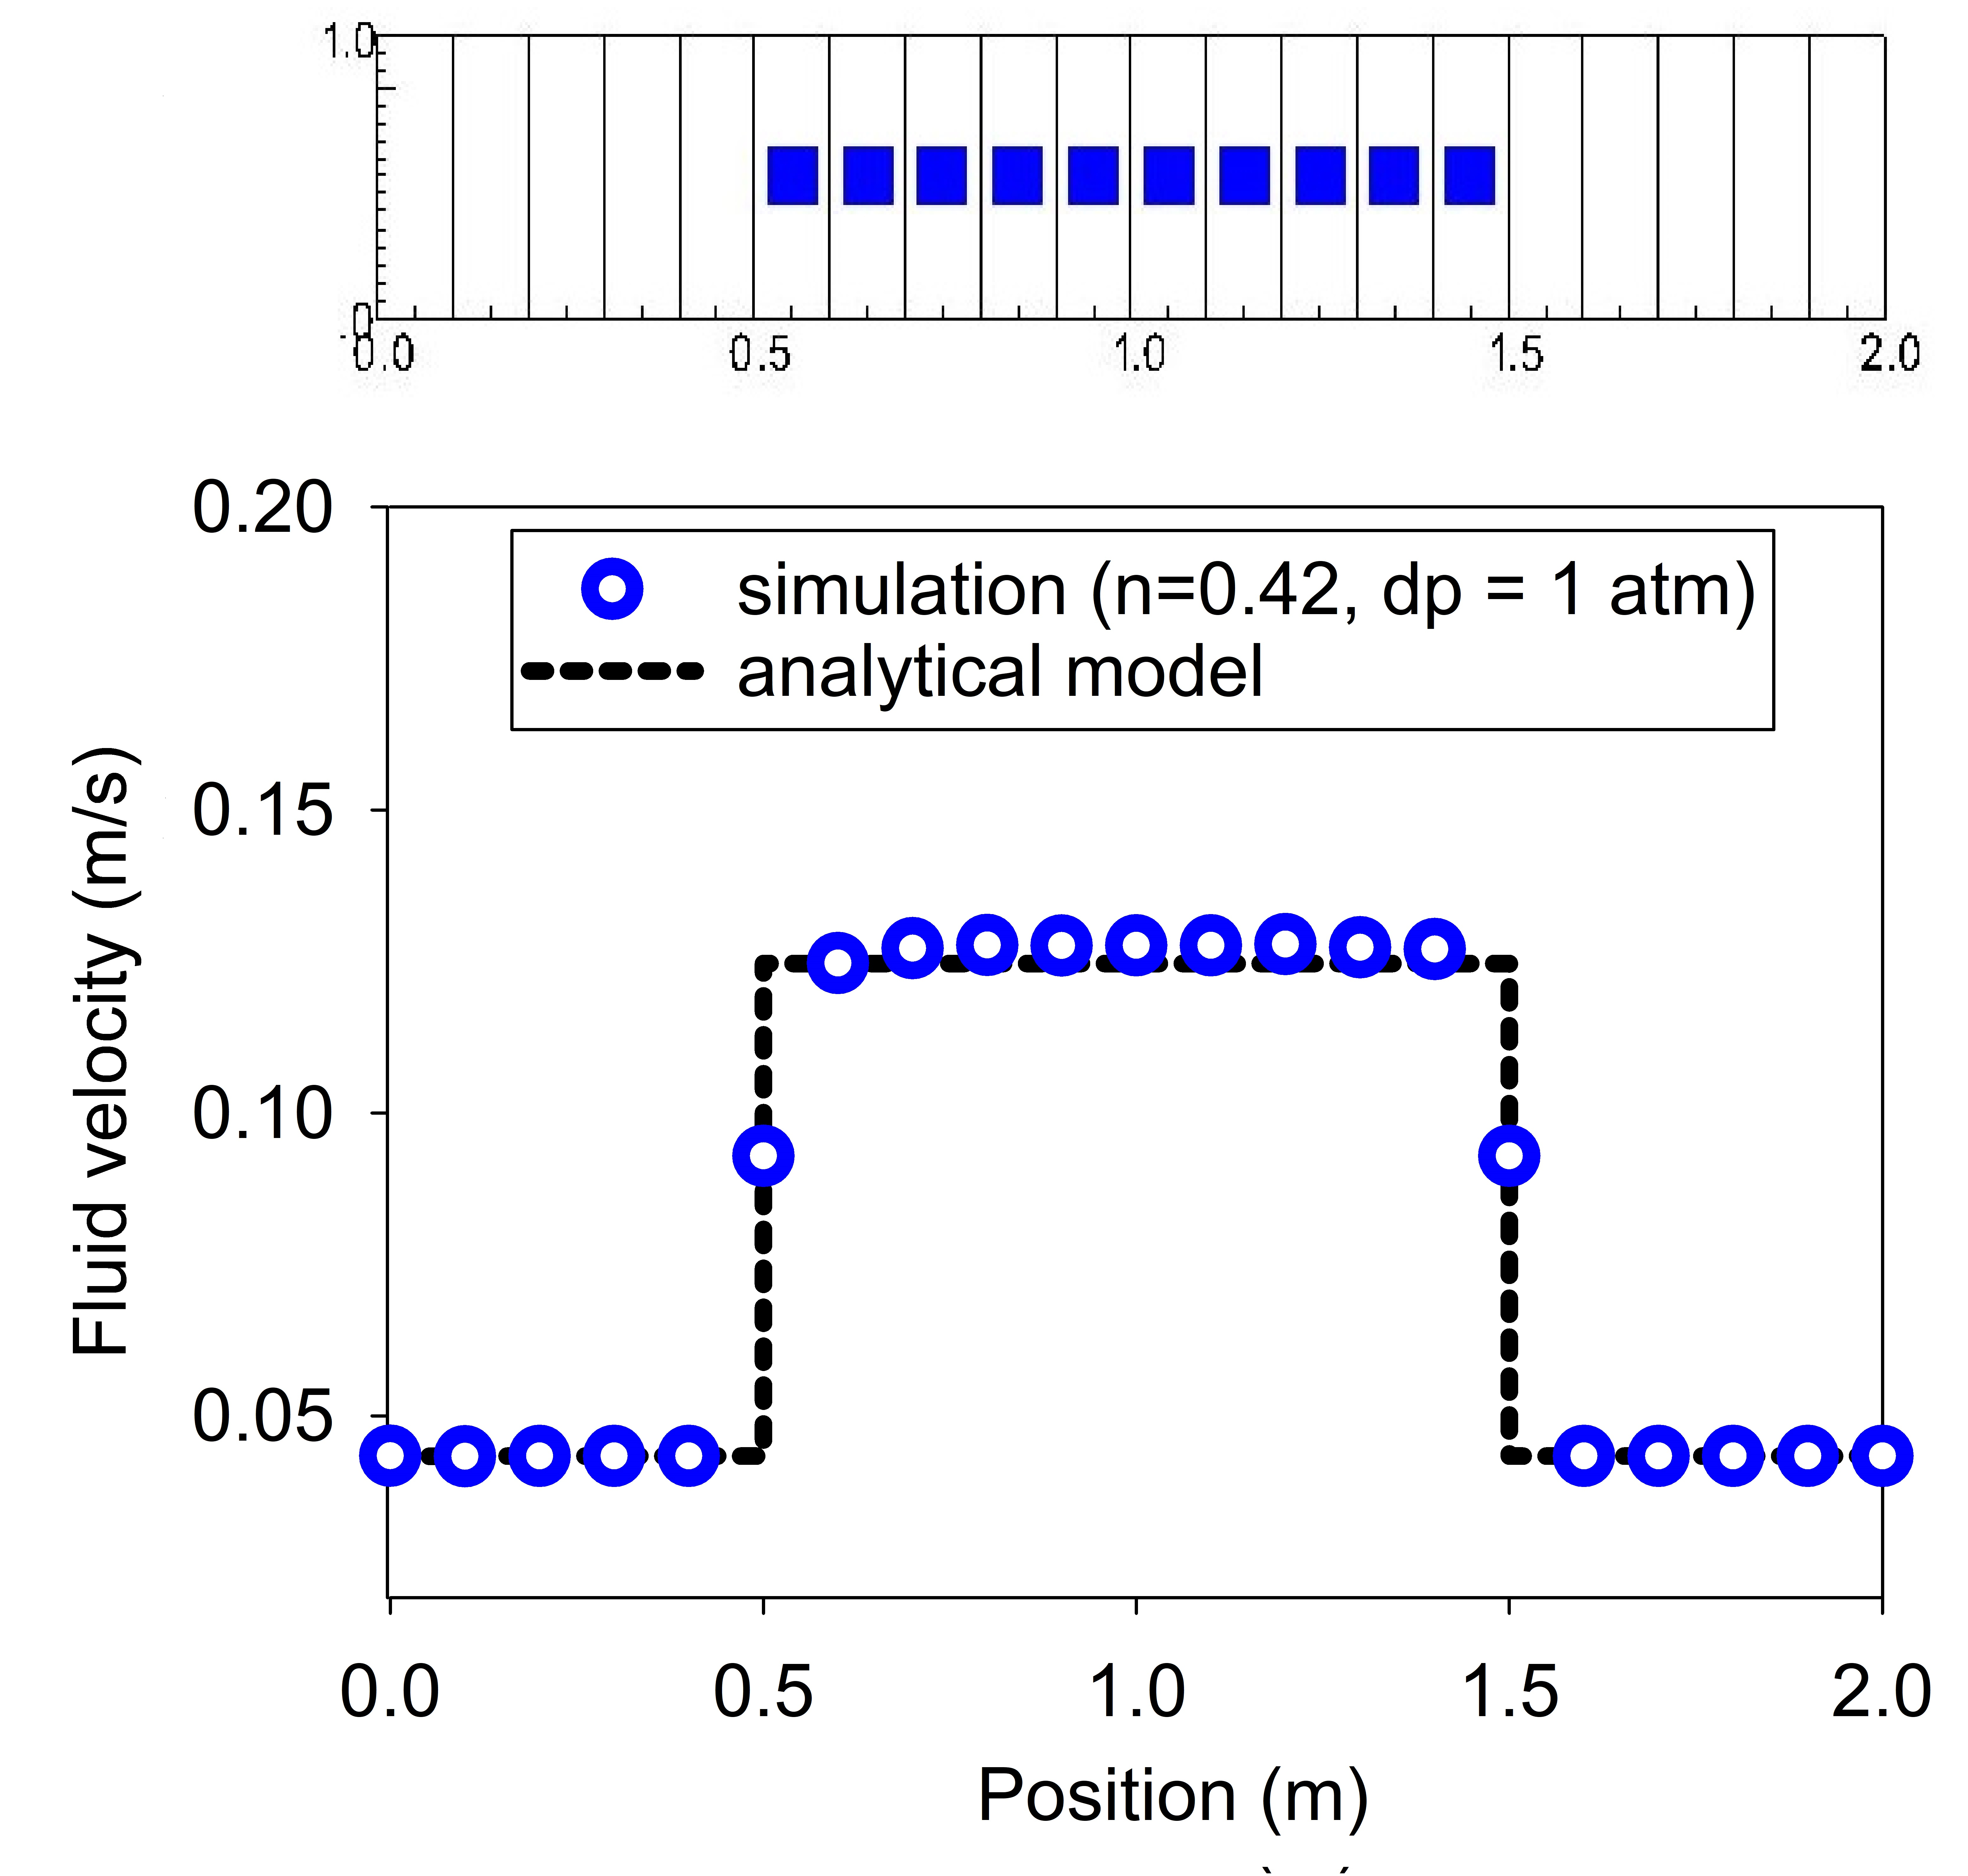
\includegraphics[width=\linewidth]{porousflow1.jpg}
\caption{Discretization of the model}
\label{fig:3c}
\end{subfigure}\hfill    
\begin{subfigure}[d]{0.5\linewidth}
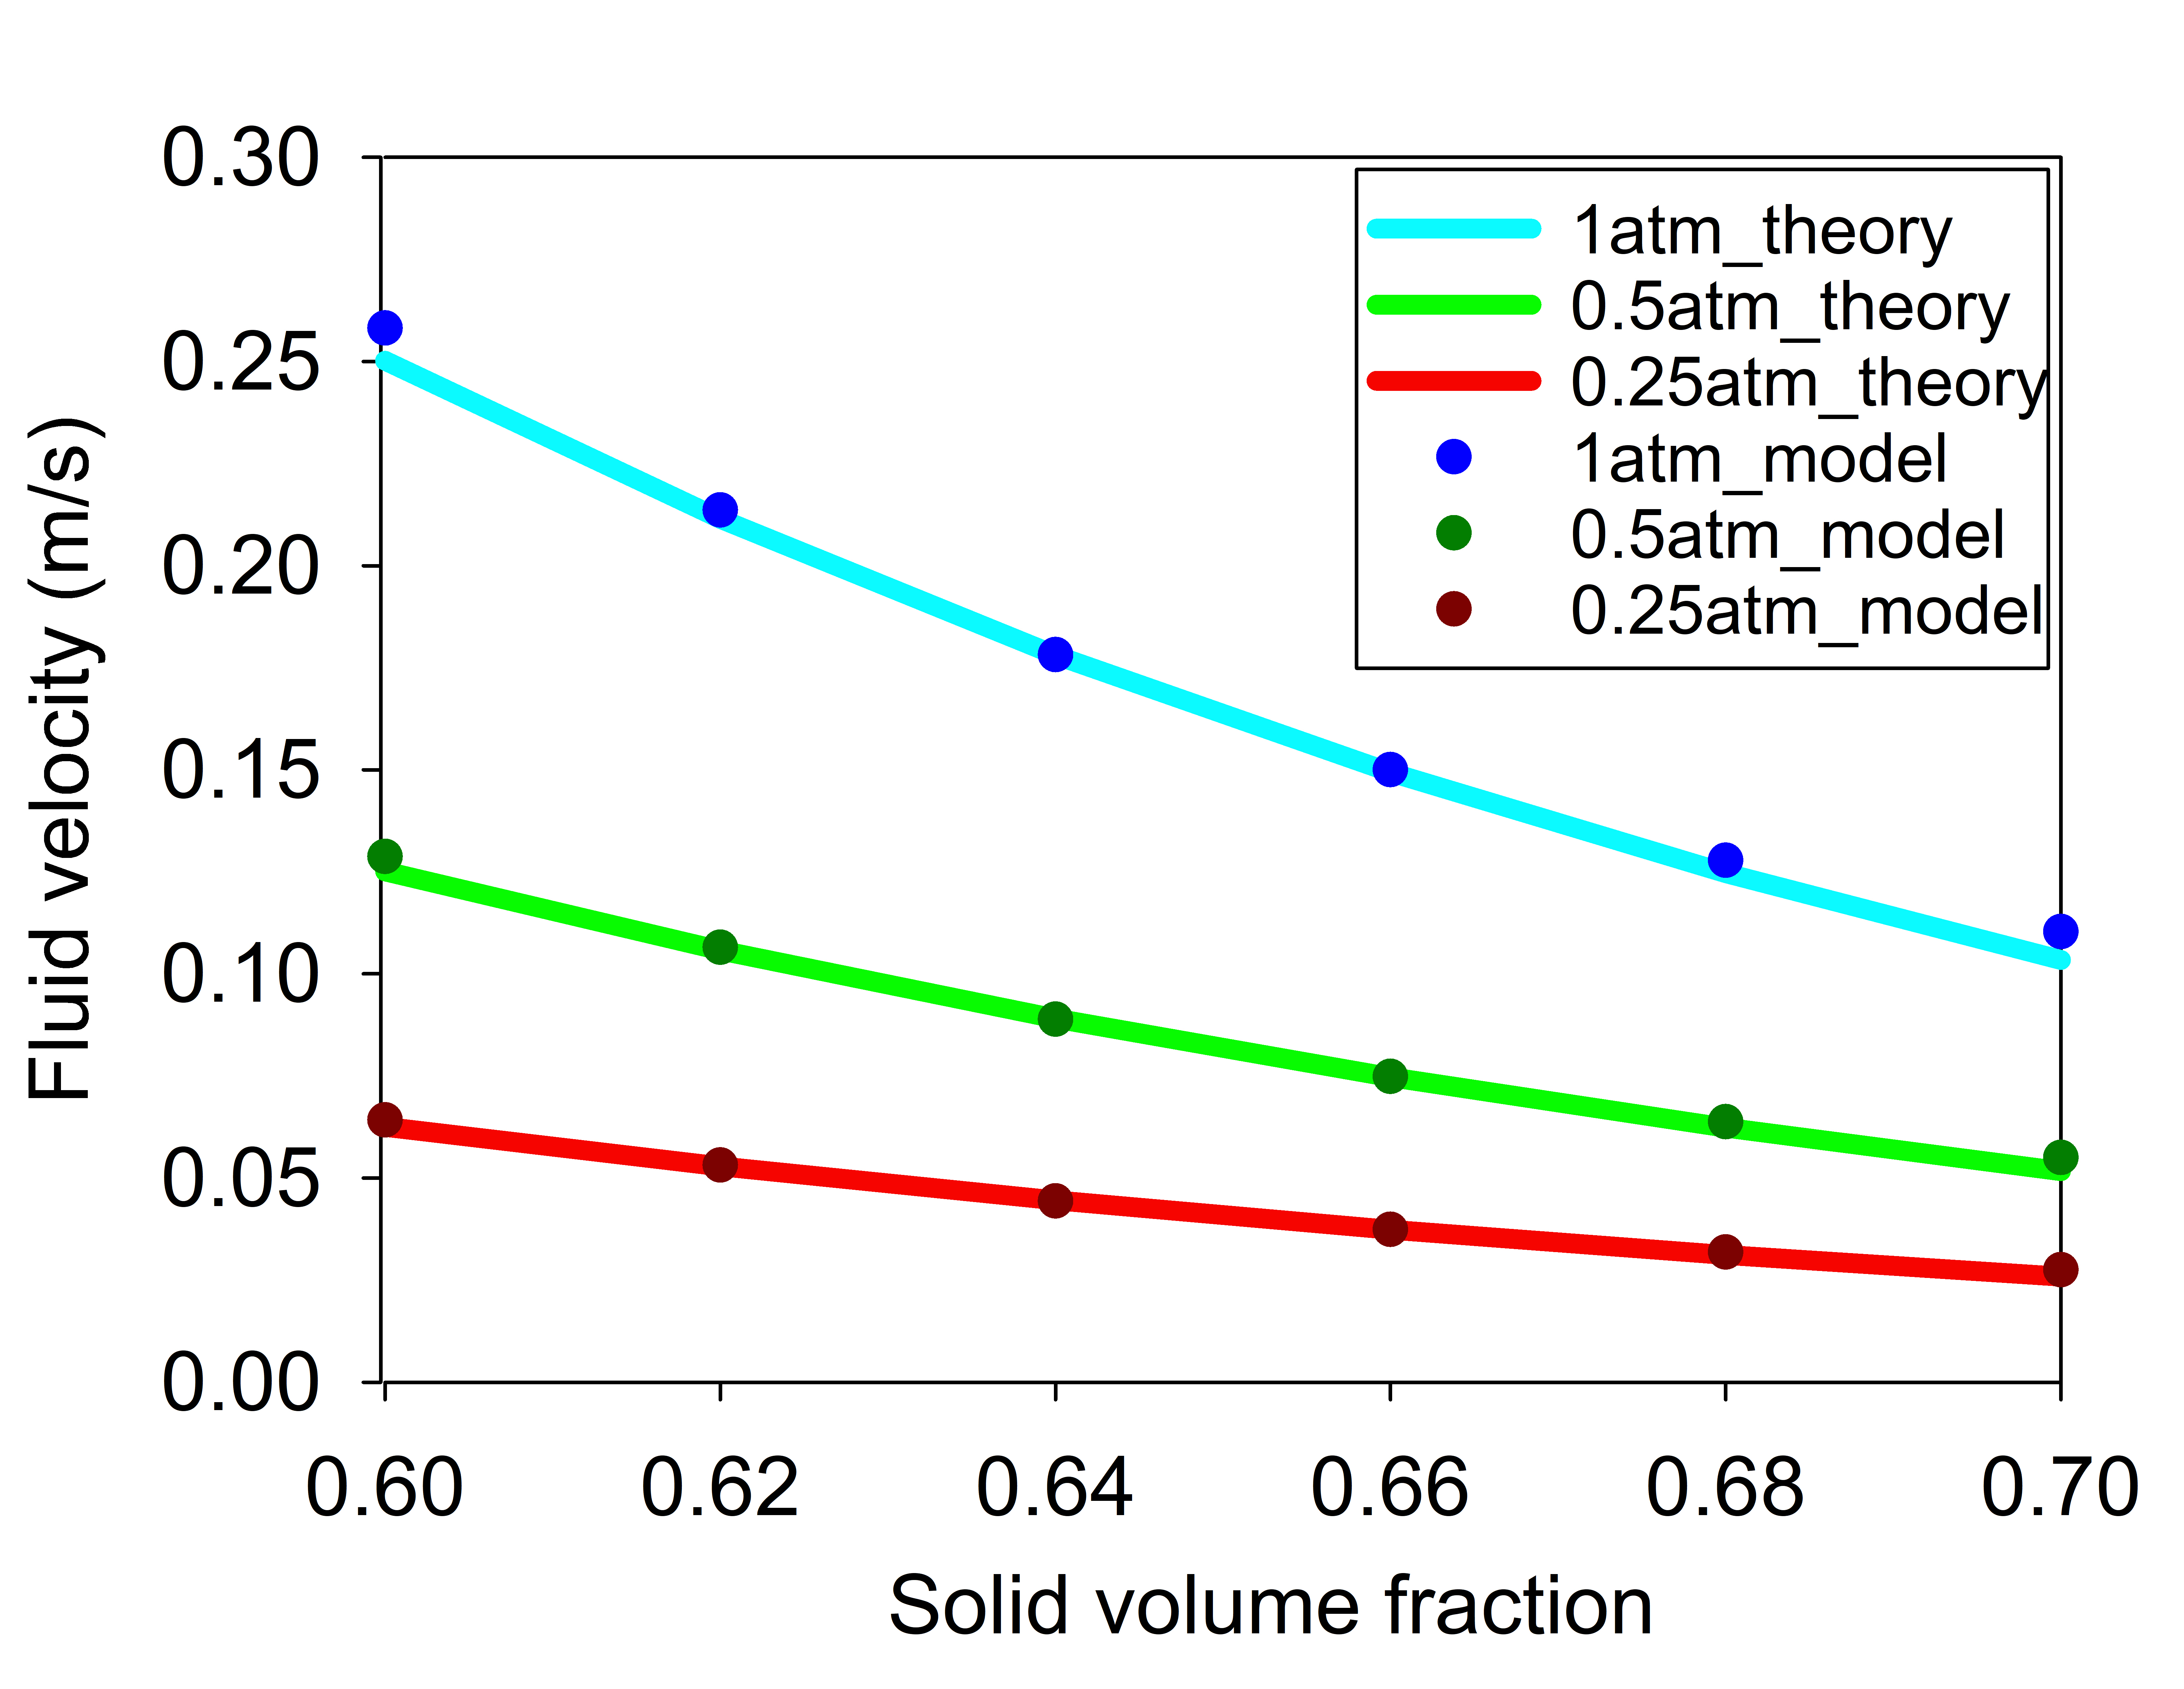
\includegraphics[width=\linewidth]{porousflow.jpg}
\caption{Comparision between analytical model and simulation}
\label{fig:3d}
\end{subfigure}
\caption{Numerical results of the fluid flow through isothermal porous media}
\label{fig:porousflow}
\end{figure}
%
%
Fluid flow through porous media is important in many engineering disciplines, like predicting water flow in soil. Fluid flow velocity in one dimension can be calculated from the porous media's hydraulic conductivity $K$ as:\\
%
%
\begin{equation}
  {U}_f   = K \frac{\Delta p_f}{L}
\end{equation}
%
%
If the Carman-Kozeny formula is adopted $F = 10\phi_s/(1-\phi_s)^2$, the hydraulic conductivity will be expressed as  $K = d^2 (1-\phi_s)^3 / 180 \mu \phi_s^2$. Then, the analytical formula of average velocity in one dimension through the porous media is:\\
%
%
\begin{equation}
  {U}_f  = \frac{1}{n} \frac{d^2 (1-\phi_s)^3}{180 \mu \phi_s^2} \frac{\Delta p_f}{L}
\end{equation}

%
%
Our numerical model is validated by modeling fluid flow through a 1m long porous media. This fluid has water properties (bulk modulus is 2GPa, density is 998 kg/m3 at 5 degrees Celsius and 10325 Pa (1atm) pressure, dynamic viscosity $\mu$ is 1mPa s). The porous media is modeled by elastic material with Young's modulus is 10 MPa, Poisson's ratio is 0.3, and density is 2650 kg/m3. The volume fraction of porous media $\phi_s$ is [0.6, 0.62, 0.66, 0.68, 0.7] and the average grain diameter $d$ is 1mm. The model is discretized in 20 finite element and the porous media in 10 finite element with 1 material point per element. The pressure gradient is applied with three different value [0.25, 0.5, 1] atm. Figure \ref{fig:porousflow} shows a good agreement of fluid flow prediction between the theory and the model. \\
%
%_______________________________
\subsection{\textsf{Isothermal consolidation}}
%
%
\begin{figure}[h]
\center
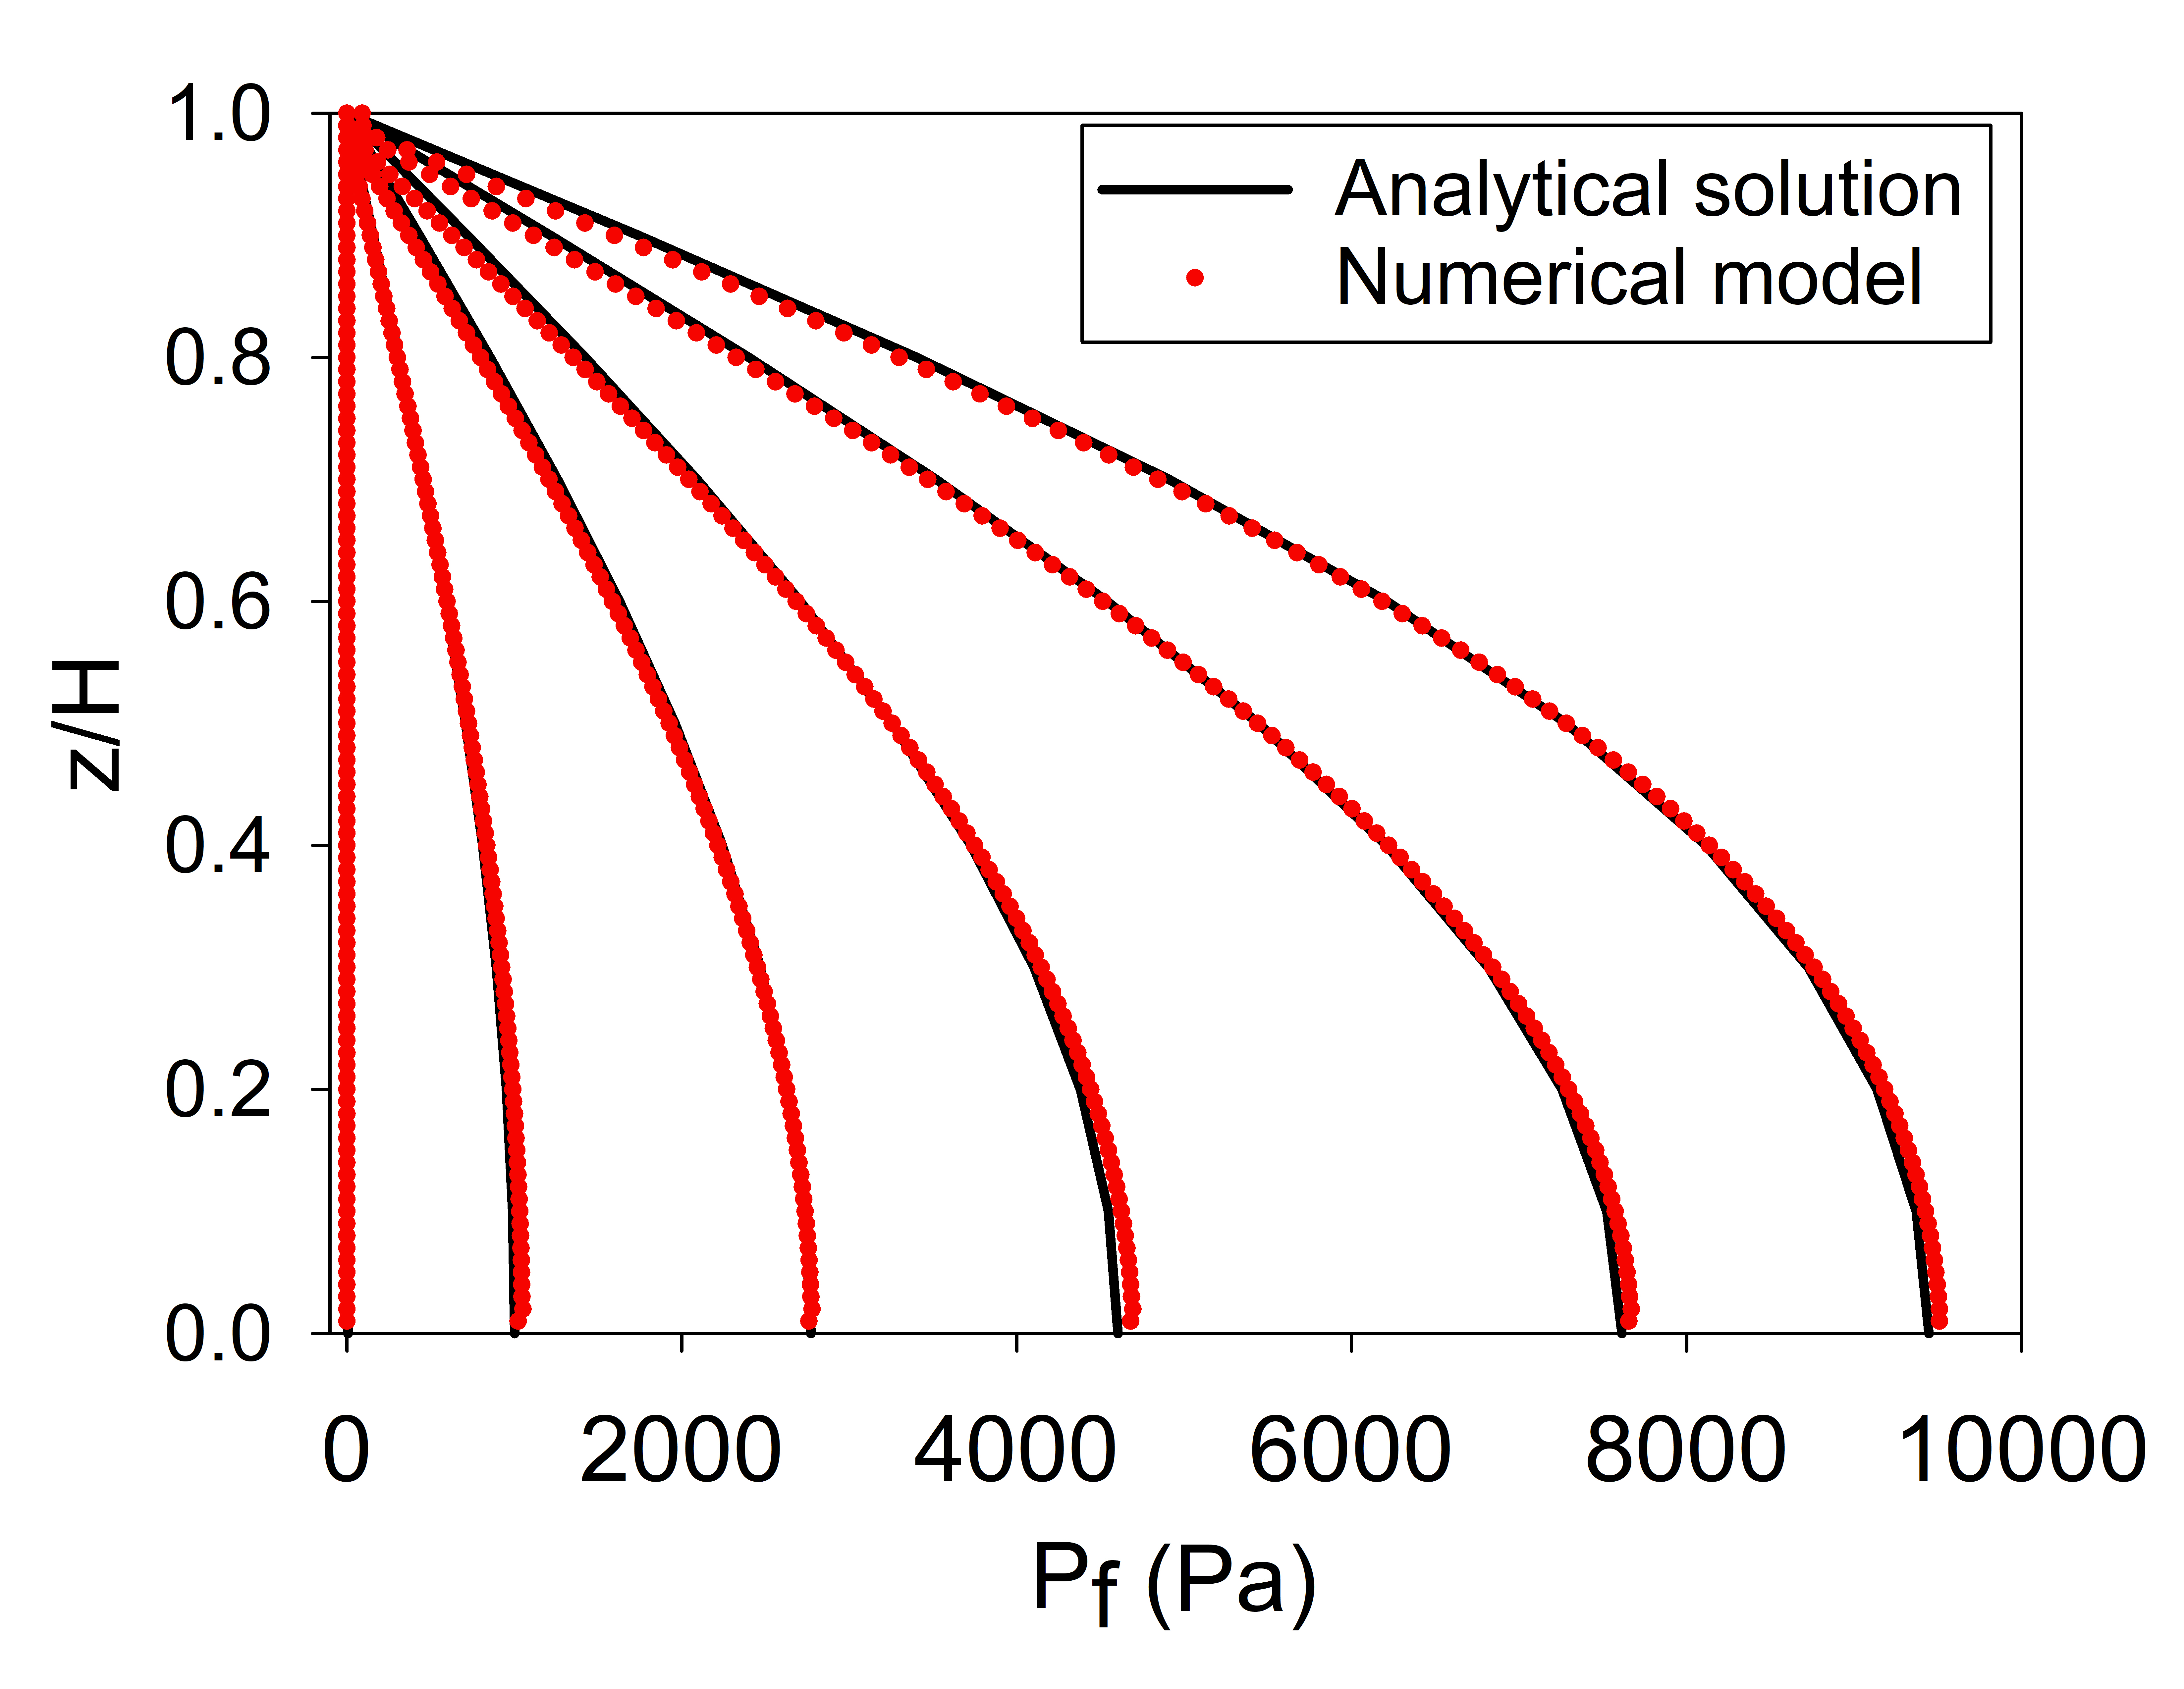
\includegraphics[scale=.3]{consolidation.jpg}
\caption{Compasion between analytical solution and numerical solution}
\label{fig:consolidation}
\end{figure}
%
%
A common benchmark fo a fully saturated porous meida is the simulation of one-dimensional consolidation. Using the Carman-Kozeny formula, the time-dependent pressure can be caluated as:
%
%
\begin{equation}
  p_f  = \sum_{m=1}^{\infty} \frac{2F_{ext}}{M} \sin (\frac{Mz}{H}) e^{-M^2T_V} \textrm{    with    }   M = \frac{\pi}{2} (2m+1)
\end{equation}
%
%
where the consolidation rate $T_v =C_vt/H^2$, the consolidation coefficient $C_v = E_v n^3 d^2/(180(1-n)^2\mu) $ and the Oedometer modulus $E_v = E(1-\upsilon)/(1+\upsilon)/(1-2\upsilon)$.
Our numerical model is validated by modeling the consolidation of a 1m column. This fluid has water properties (bulk modulus is 2GPa, density is 998 kg/m3 at 5 degrees Celsius and 10325 Pa (1atm) pressure, dynamic viscosity $\mu$ is 1mPa s). The porous media is modeled by elastic material with Young's modulus is 10 MPa, Poisson's ratio is 0.3, and density is 2650 kg/m3. The volume fraction of porous media $\phi_s$ is 0.7 which is equivalent to the porosity of 0.3 and the average grain diameter $d$ is 1mm. The model is discretized in 100 finite element with 1 material point per element. The external pressure applies to the top of the column is 10 kPa. Figure \ref{fig:consolidation} shows a good agreement of fluid flow prediction between the theory and the model. \\
%_______________________________
\subsection{\textsf{Thermal induced cavity flow}}
%
%
\begin{figure}
\center
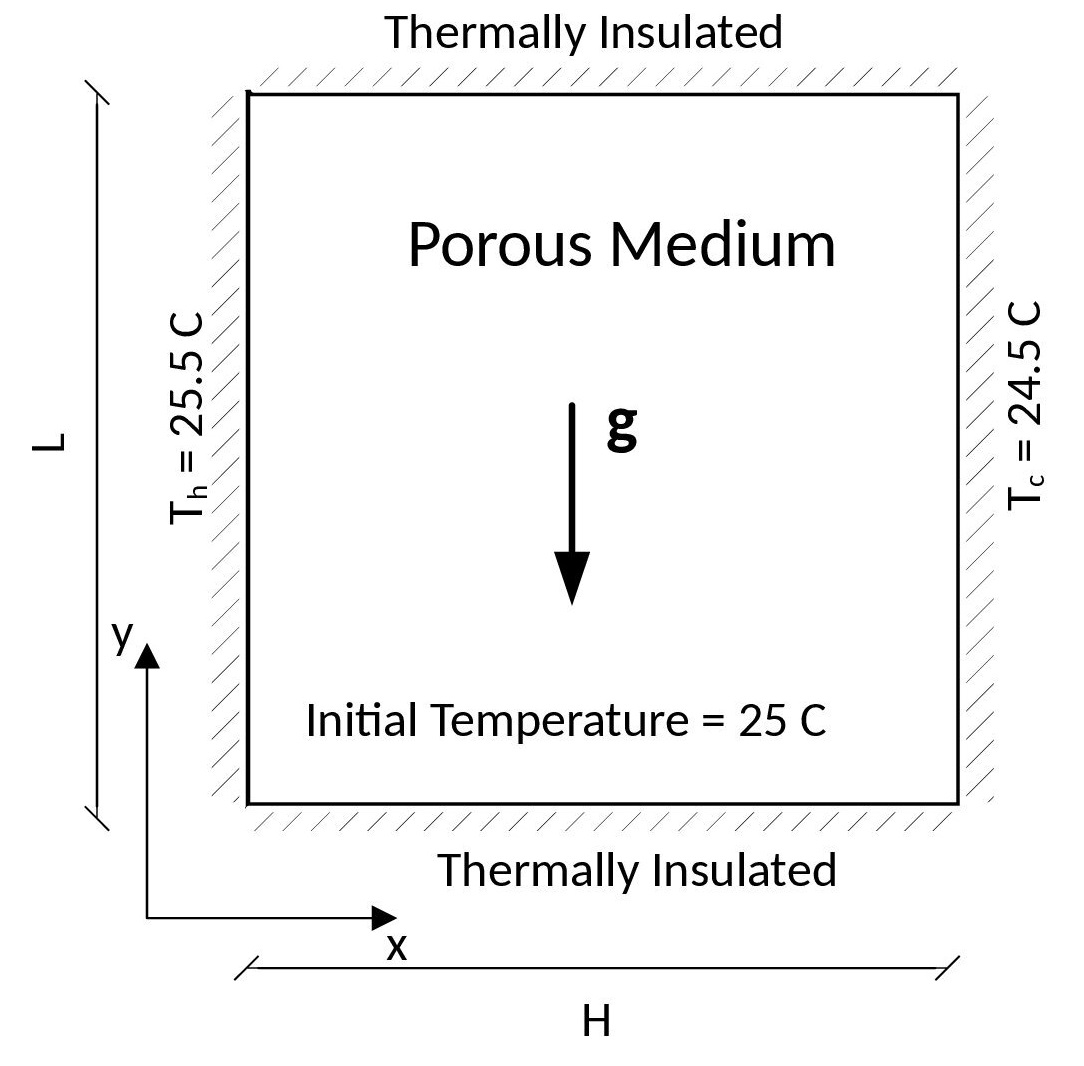
\includegraphics[scale=.5]{box_thermal.jpg}
\caption{Model schematic}
\label{fig:thermalModel}
\end{figure}
%
%
\begin{figure}
\center
%add desired spacing between images, e. g. ~, \quad, \qquad, \hfill etc. 
%(or a blank line to force the subfigure onto a new line)
\begin{subfigure}[c]{0.5\linewidth}
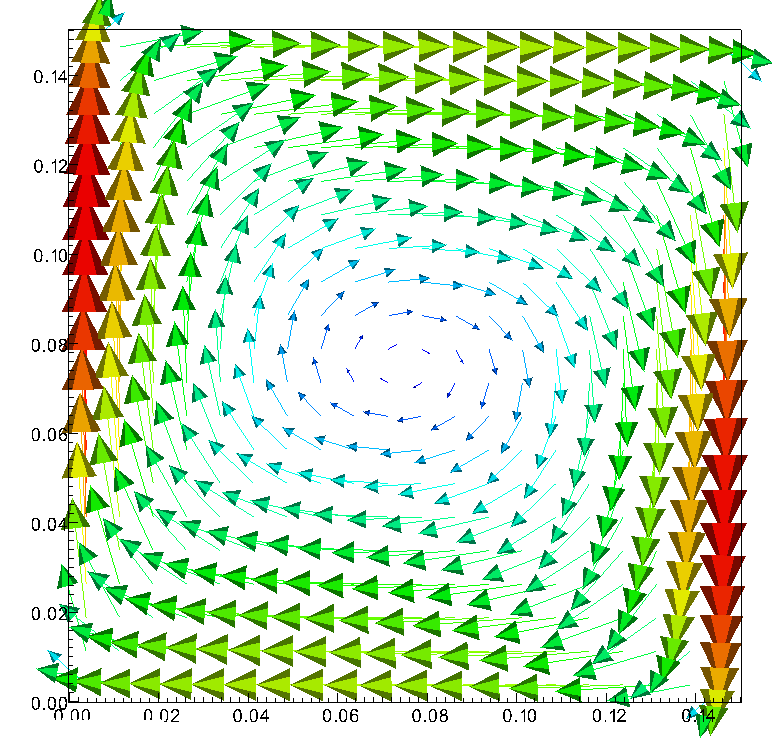
\includegraphics[width=\linewidth]{thermal.png}
\caption{MPMICE2 model}
\end{subfigure}\hfill    
\begin{subfigure}[d]{0.5\linewidth}
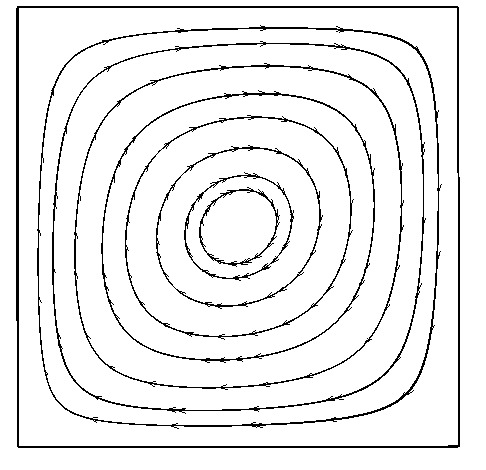
\includegraphics[width=\linewidth]{velocity_thermal-1.jpg}
\caption{FEM model}
\end{subfigure}
\caption{Comparision between MPMICE2 model and FEM model}
\label{fig:thermal}
\end{figure}
%
%
Another benchkmark is the thermal induced cavity flow in porous media. Temperature and velocity distributions are calculated for a square non-deformable saturated porous media The top and bottom walls are insulated, and the left and right walls are at fixed temperatures differing by 1 C. The fluid motion at stead state are cavity flow due to the temperature induced density variation. \\
The numerical is validated by comparing with the numerical solution of the finite element method. The fluid has water properties (bulk modulus is 2GPa, density is 998 kg/m3 at 5 degrees Celsius and 10325 Pa (1atm) pressure, dynamic viscosity $\mu$ is 1 mPa s). The porous media is modeled by non deformable material, and density is 2500 kg/m3. The specific heat capacity of the water and porous skeleton are 4181 J/kg.K and 835 J/kg.K respectively. The thermal conductivity of the water and porous skeleton are 0.598 W/m.K and 0.4 W/m.K. The volume fraction of porous media $\phi_s$ is 0.6 which is equivalent to the porosity of 0.4 and the average grain diameter $d$ is 1mm. The model is discretized in 20 x 20 finite element with 4 material point per element. Figure \ref{fig:thermal} shows a good agreement of numerical results of the model compared with the numerical solution of the finite element method. \\
%_______________________________
\subsection{\textsf{Underwater debris flow}}
%
%
\begin{figure}[h]
\center
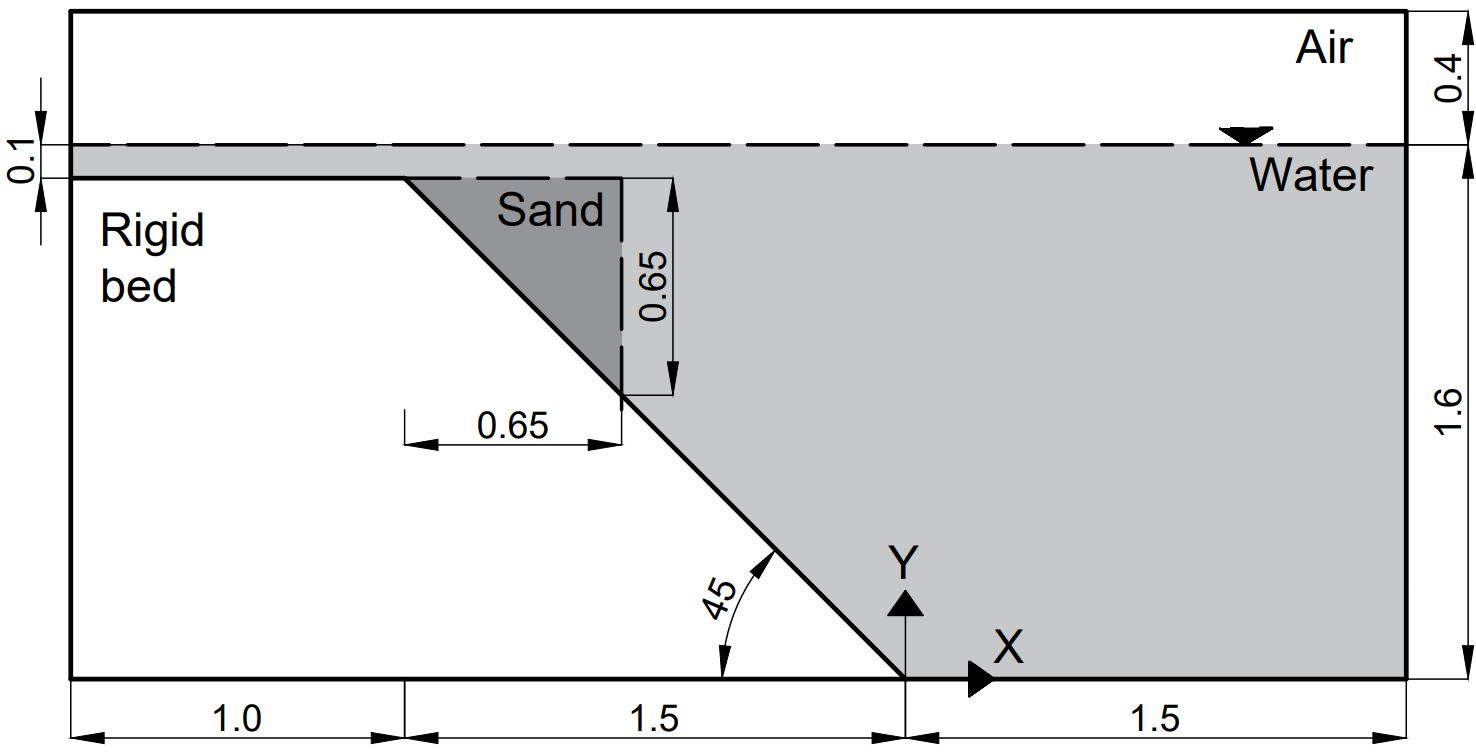
\includegraphics[scale=.3]{SandBoxscheme.jpg}
\caption{Model schematic}
\label{fig:SandBoxModel}
\end{figure}
%
%
The numerical example is validated by Rzadkiewicz et al.'s experiment on submarine debris flow \cite{Rzadkiewicz}. During the experiment, sand in a triangular box is released and then slides along a rigid bed inclined 45 degrees under water, see Figure \ref{fig:SandBoxModel}.\\
%
%
\begin{figure}
\center
%add desired spacing between images, e. g. ~, \quad, \qquad, \hfill etc. 
%(or a blank line to force the subfigure onto a new line)
\begin{subfigure}[c]{0.5\linewidth}
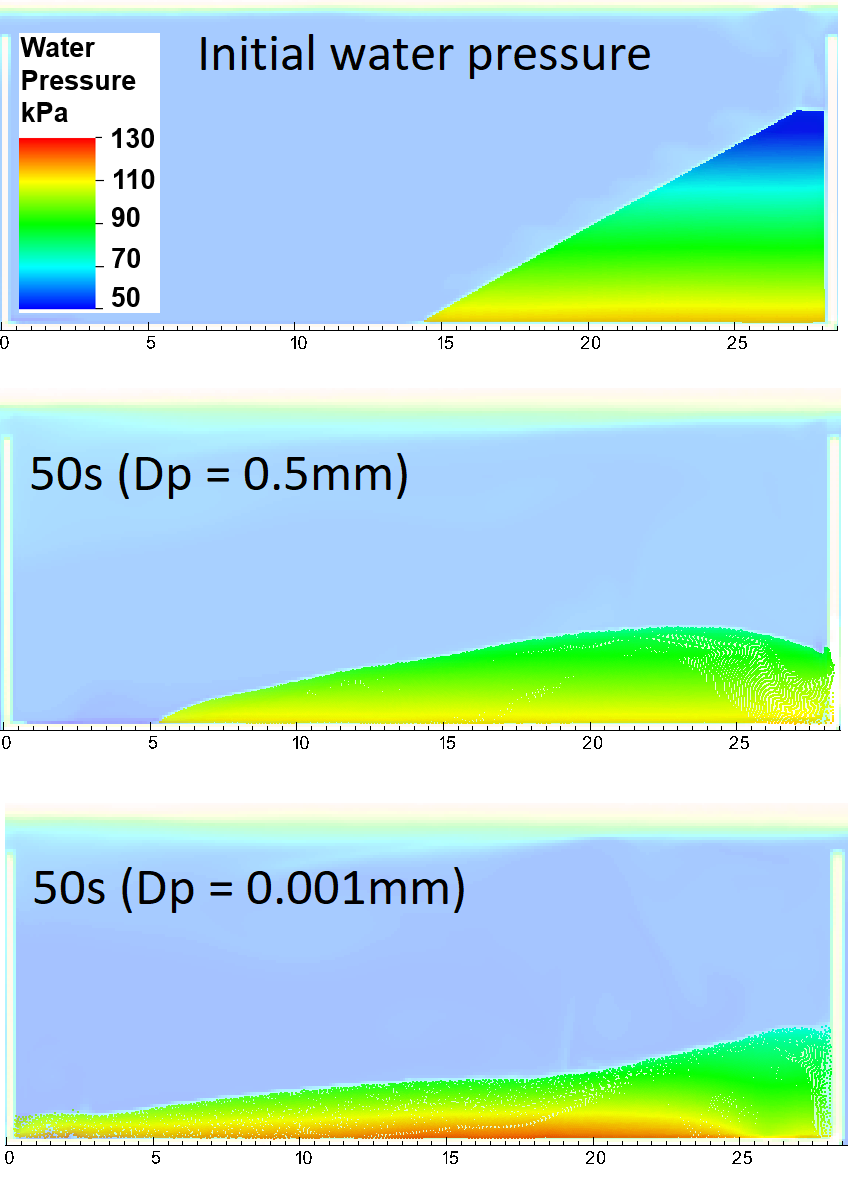
\includegraphics[width=\linewidth]{1.jpg}
\caption{0.4 seconds}
\label{0.4s}
\end{subfigure}\hfill    
\begin{subfigure}[d]{0.5\linewidth}
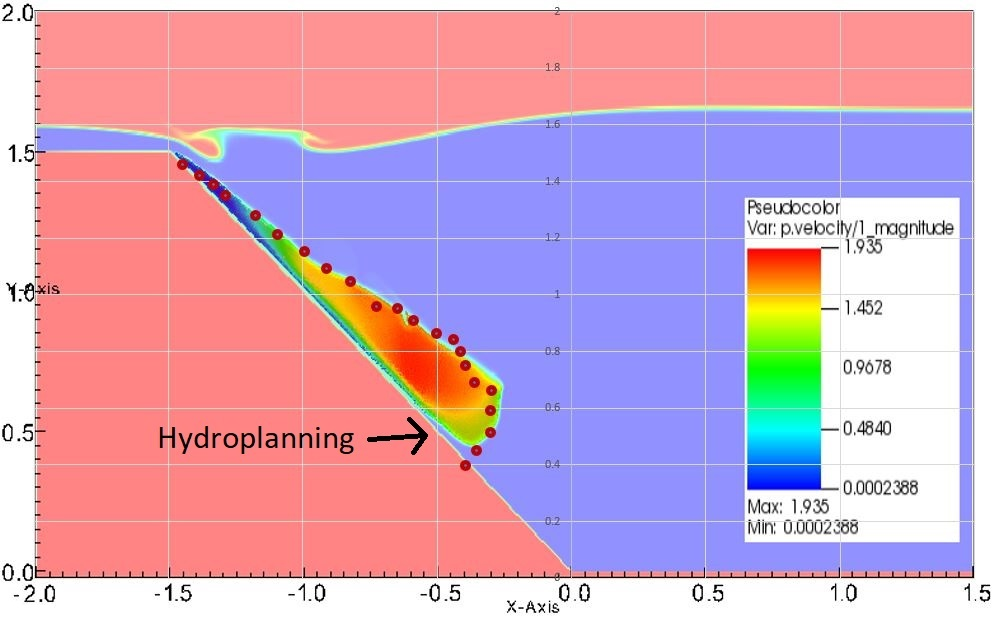
\includegraphics[width=\linewidth]{2.jpg}
\caption{0.8 seconds}
\label{0.8s}
\end{subfigure}
\caption{Simulation of underwater debris flow}
\label{fig:debris}
\end{figure}
%
%
\begin{table}[h]
\center
\begin{tabular}{|c|c|c|c|c|c|c|}
\hline
\textbf{Materials}                                                 & \textbf{\begin{tabular}[c]{@{}c@{}}Bulk \\ modul\\ (Pa)\end{tabular}} & \textbf{\begin{tabular}[c]{@{}c@{}}Shear \\ modul\\ (Pa)\end{tabular}} & \textbf{\begin{tabular}[c]{@{}c@{}}Density\\ (kg/m3)\end{tabular}} & \textbf{\begin{tabular}[c]{@{}c@{}}Temp\\ (C)\end{tabular}} & \textbf{\begin{tabular}[c]{@{}c@{}}Dynamic \\ vicosity\\ (Pa s)\end{tabular}} & \textbf{\begin{tabular}[c]{@{}c@{}}Yield \\ stress\\ (Pa)\end{tabular}} \\ \hline
\begin{tabular}[c]{@{}c@{}}Water\\ (at surface)\end{tabular}       & 2.15e9                                                                  & -                                                                        & 999.8                                                              & 5                                                           & 855e-6                                                                        & -                                                                       \\ \hline
\begin{tabular}[c]{@{}c@{}}Air\\ (at top \\ boundary)\end{tabular} & -                                                                       & -                                                                        & 1.177                                                              & 5                                                           & 18.45e-6                                                                      & -                                                                       \\ \hline
\begin{tabular}[c]{@{}c@{}}Sand\\ (porous \\ media)\end{tabular}   & 8.33e6                                                                  & 20e6                                                                     & 1985                                                               & 5                                                           & -                                                                             & 200                                                                     \\ \hline
\begin{tabular}[c]{@{}c@{}}Rigid bed\\ (solid)\end{tabular}        & 117e7                                                                 & 43.8e7                                                                   & 8900                                                               & 5                                                           & -                                                                             & -                                                                       \\ \hline
\end{tabular}
\caption{Numerical parameters for the underwater submarine debris}
\label{table2}
\end{table}
In the numerical model, the material properties are selected based on the experiment by Rzadkiewicz et al \cite{Rzadkiewicz}. Sand has a saturated density of 1985 kg/m3 and yield stress of 200 Pa. Young's modulus has little effect on debris flow run-out because of the extreme large deformation of the debris. Therefore, we select 50 MPa Young's modulus with 0.25 Poisson's ratio. The rigid bed is much stiffer with bulk modulus and shear modulus of $117e^7$ Pa and $43.8e^7$ Pa. Under gravity, the density of the water at the surface is 999.8 $kg/m^3$ at the pressure of 1 atm. At the top boundary, the air has a density of 1.17 $kg/m^3$ at the atmospheric pressure of 1 atm. At 5 Celcius degrees, air and water have viscosity of $18.45e^{-3}$  mPa s and 1  mPa s respectively. The numerical parameters used in this example are presented in Table \ref{table2}.   \\
On all boundary faces, the Dirichlet boundary condition is imposed for velocity (u = 0 m/s) and temperature (T = 5 Celcius degrees), while the Neuman boundary condition is imposed at the top boundaryfor pressure (dp/dx = 0 kPa) and density (d/dx = 0 $kg/m^3$). For the background mesh, there are 700 x 400 = 280.000 cells. In each cell of the debris flow and rigid bed, there are 2 x 2 material points. \\
%
%
\begin{figure}
\center
%add desired spacing between images, e. g. ~, \quad, \qquad, \hfill etc. 
%(or a blank line to force the subfigure onto a new line)
\begin{subfigure}[c]{0.5\linewidth}
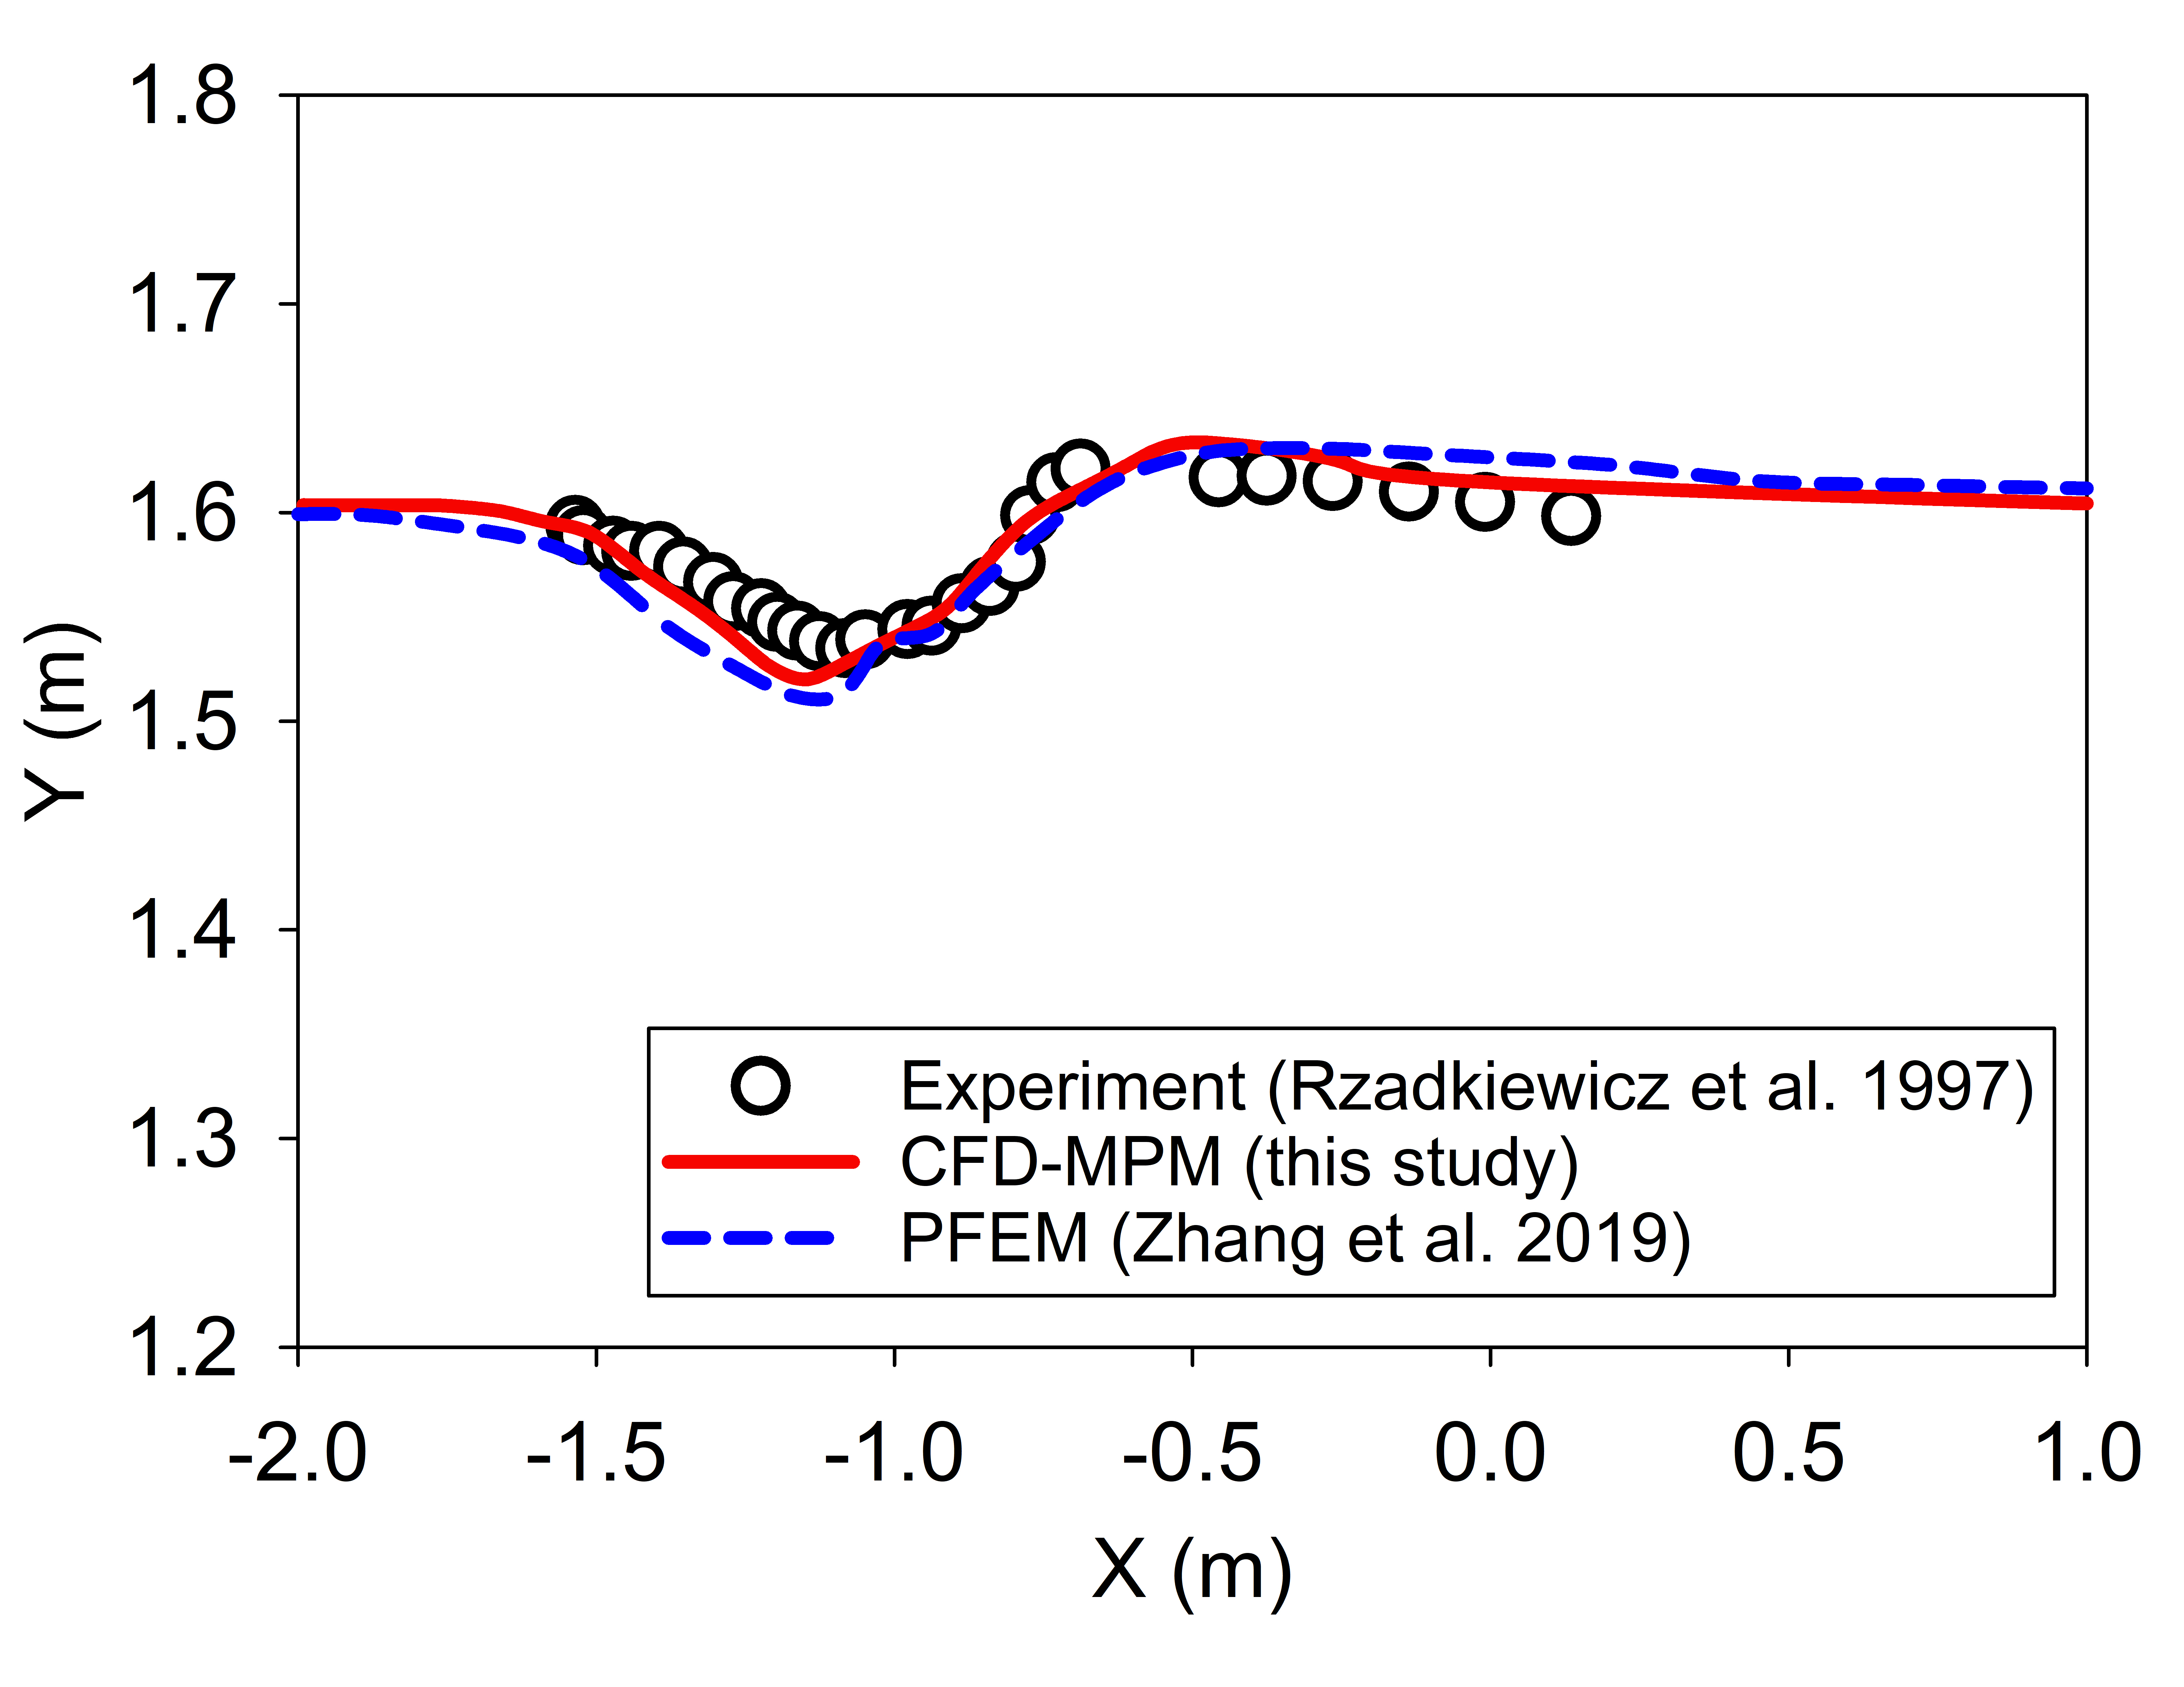
\includegraphics[width=\linewidth]{0.4swater.jpg}
\caption{0.4 seconds}
\label{0.4swater}
\end{subfigure}\hfill    
\begin{subfigure}[d]{0.5\linewidth}
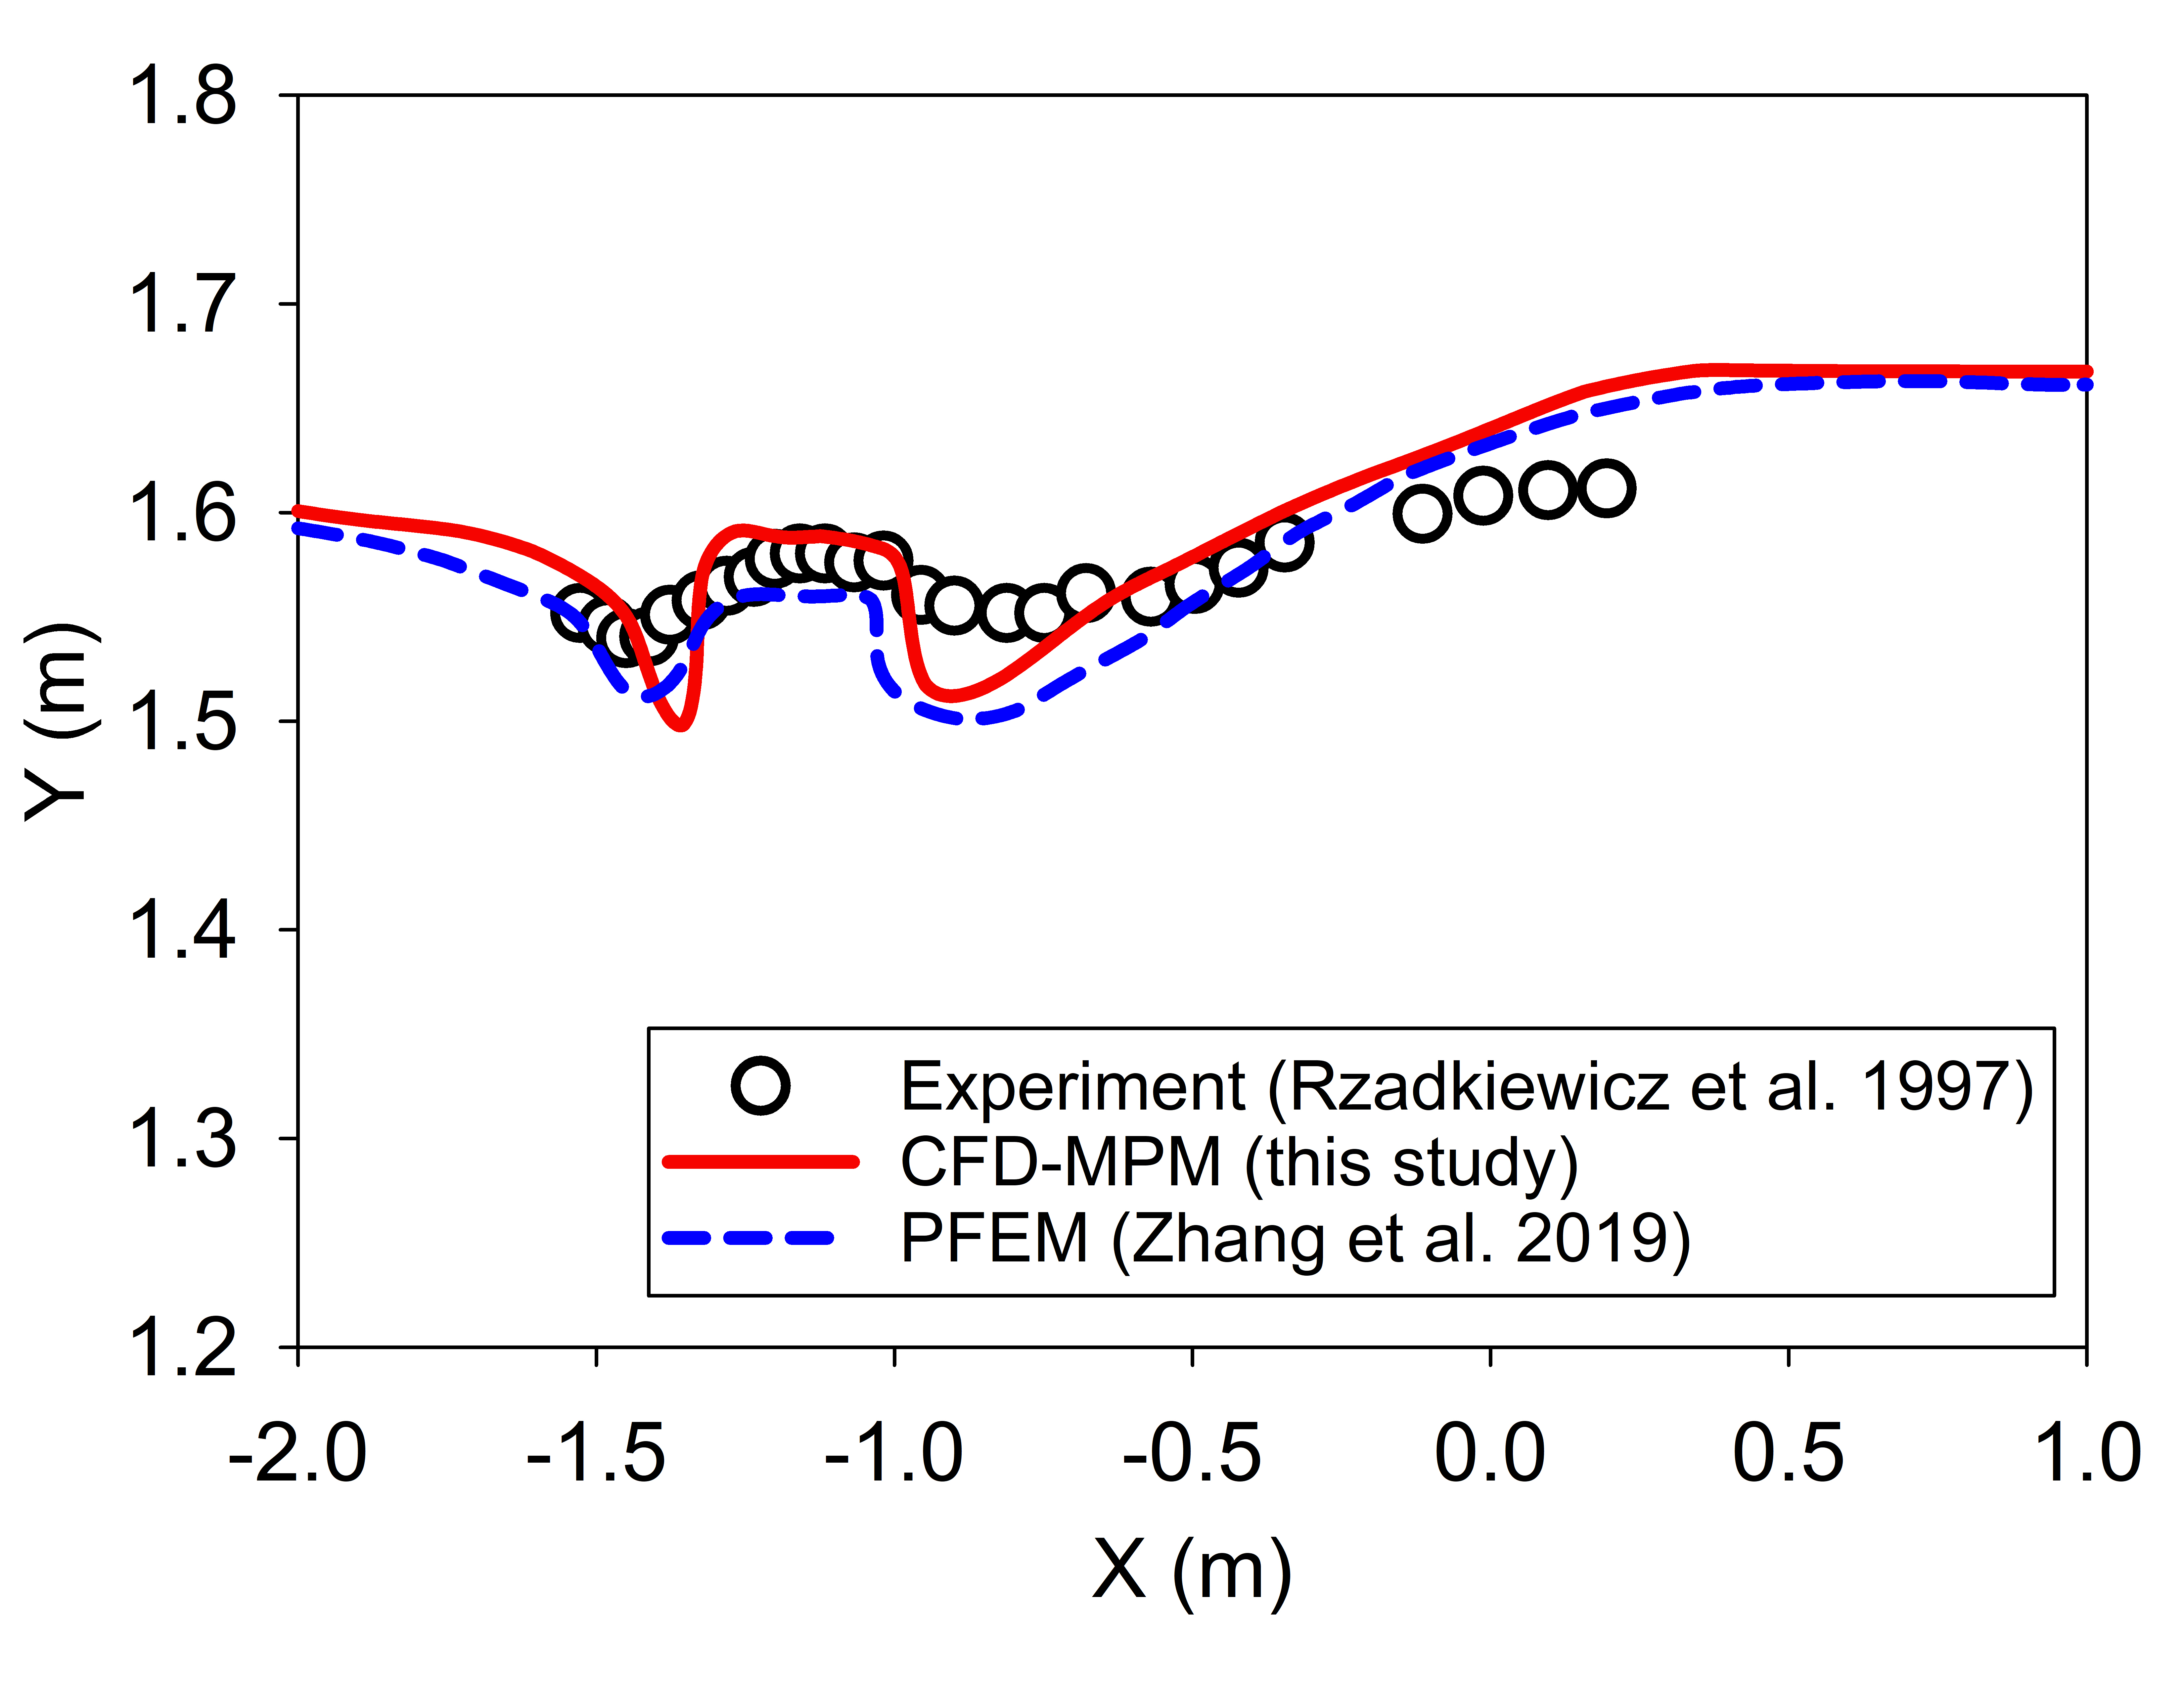
\includegraphics[width=\linewidth]{0.8swater.jpg}
\caption{0.8 seconds}
\label{0.8swater}
\end{subfigure}
\caption{Simulation of underwater debris flow}
\label{watersurface}
\end{figure}
%
%
Figure \ref{0.4s} and  \ref{0.8s} show snapshots of the debris flow sliding in the plane at 0.4 s and 0.8 s. Our simulations match the computed results from Rzadkiewicz et al. \cite{Rzadkiewicz}. The model also captures typical hydroplaning mechanism of the underwater debris flow (hydroplaning means the debris flow is lifted up and no longer in contact with the bottom layer). The elevation of the free surface at 0.4s and 0.8s is compared between our proposed method and other methods in Figure \ref{watersurface}. Once again, our computed results were consistent with both the experiment and others computational results. Unlike other computational models based on total stress analysis, the proposed model based on the effective stress analysis which allows to analyze the water pressure  and temperature in the debris flow.\\
%
%
\begin{figure}
\center
%add desired spacing between images, e. g. ~, \quad, \qquad, \hfill etc. 
%(or a blank line to force the subfigure onto a new line)
\begin{subfigure}[c]{0.5\linewidth}
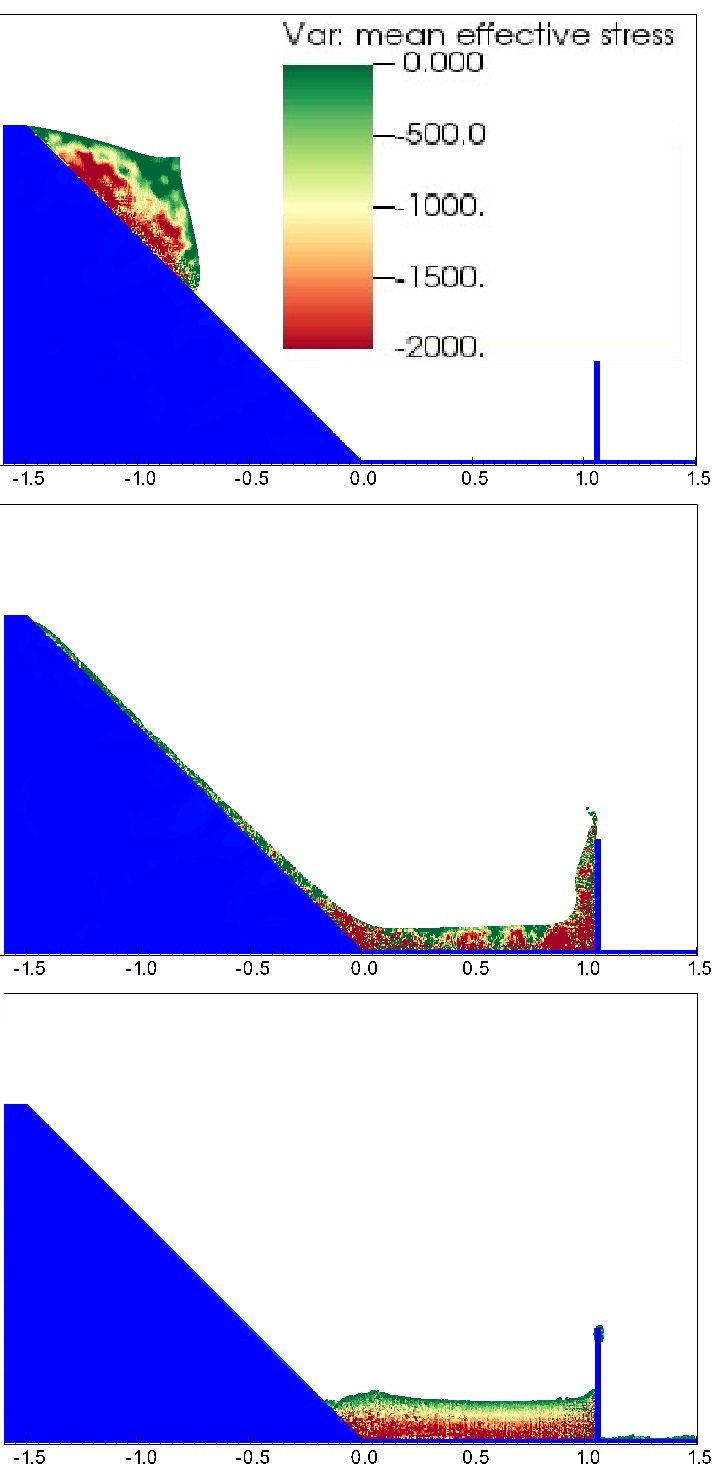
\includegraphics[width=\linewidth]{SHMPM.jpg}
\caption{saturated debris flow using MPM}
\label{saturatedflowa}
\end{subfigure}\hfill    
\begin{subfigure}[d]{0.5\linewidth}
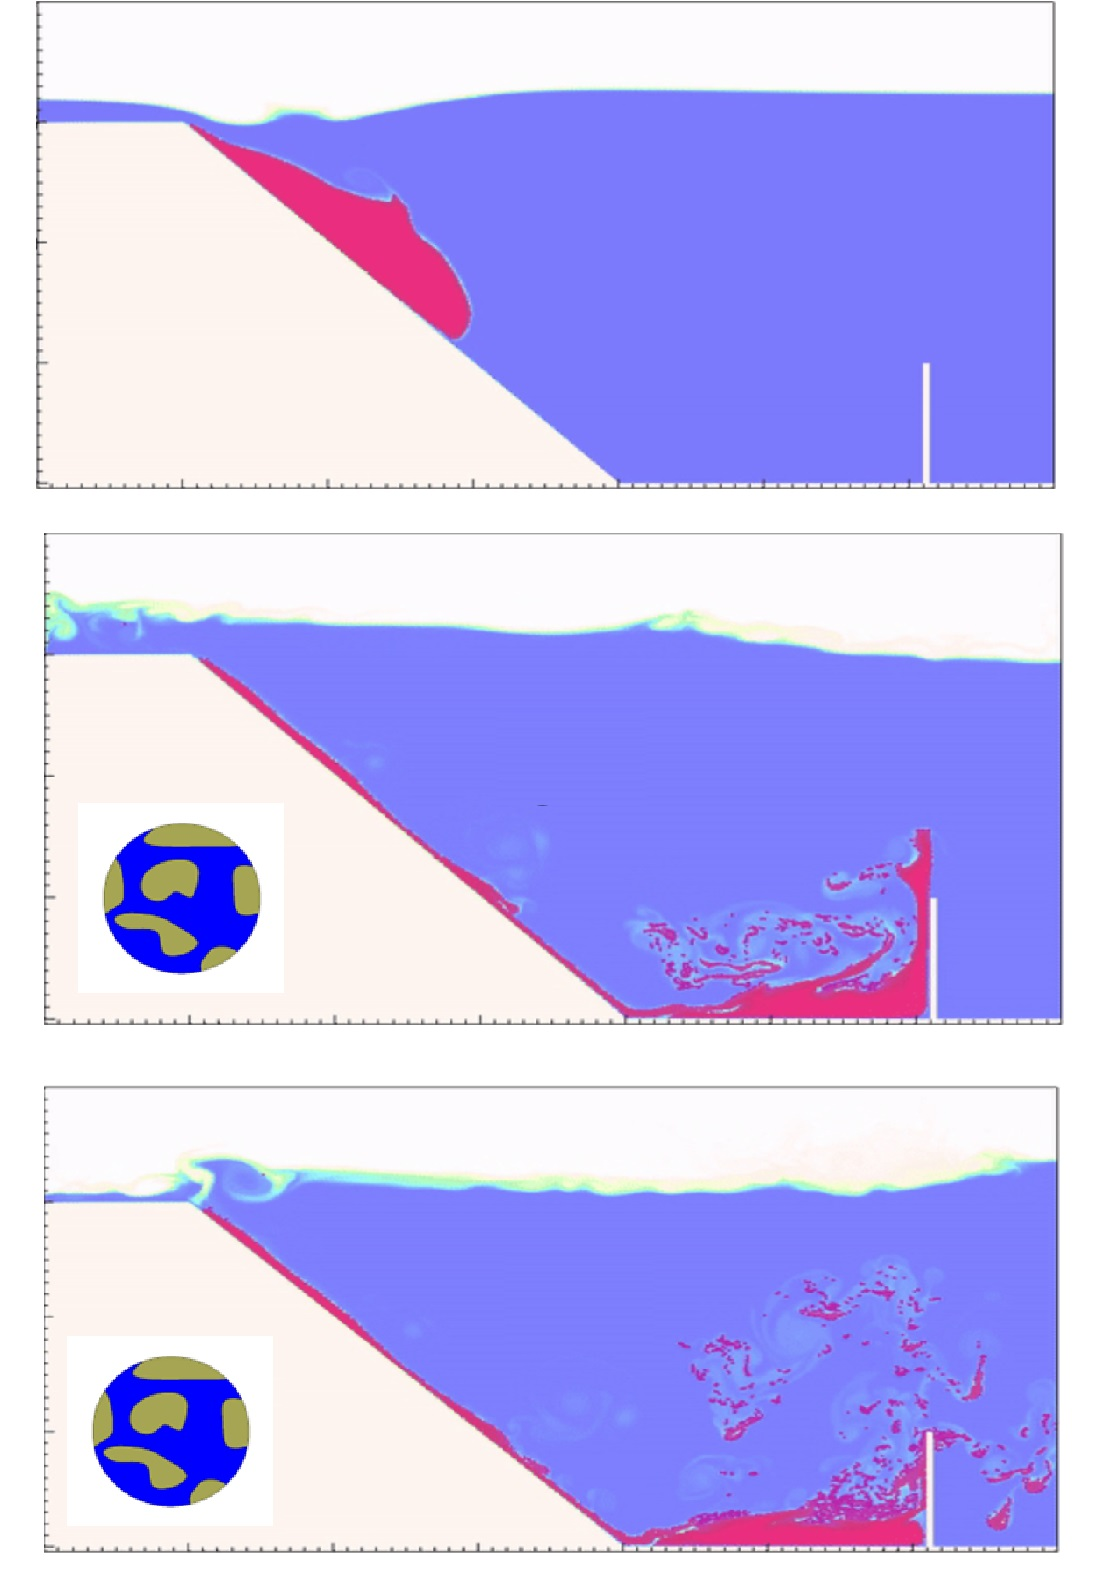
\includegraphics[width=\linewidth]{MPMICE_debris.jpg}
\caption{underwater debris flow using MPMICE}
\label{saturatedflowb}
\end{subfigure}
\caption{Simulation of underwater debris flow}
\label{saturatedflow}
\end{figure}
%
%
We also explore the difference between underwater debris flow and saturated debris flow in terms of interacting with obstacle. Figure \ref{saturatedflow} shows the snapshot of the simulations of underwater and saturated debris flow. The saturated debris flow (see Figure \ref{saturatedflowa}) behaves like frictional flow as grain have contact forces with each other. On the other hand, the underwater debris flow (see Figure \ref{saturatedflowb}) behaves like tubulent flow as grains are separated from each other and exhibit no contact forces between grains.  \\
%_______________________________
\subsection{\textsf{Earthquake-induced submarine landslides}}
%
%
\begin{figure}[h]
\center
%add desired spacing between images, e. g. ~, \quad, \qquad, \hfill etc. 
%(or a blank line to force the subfigure onto a new line)
\begin{subfigure}[c]{0.5\linewidth}
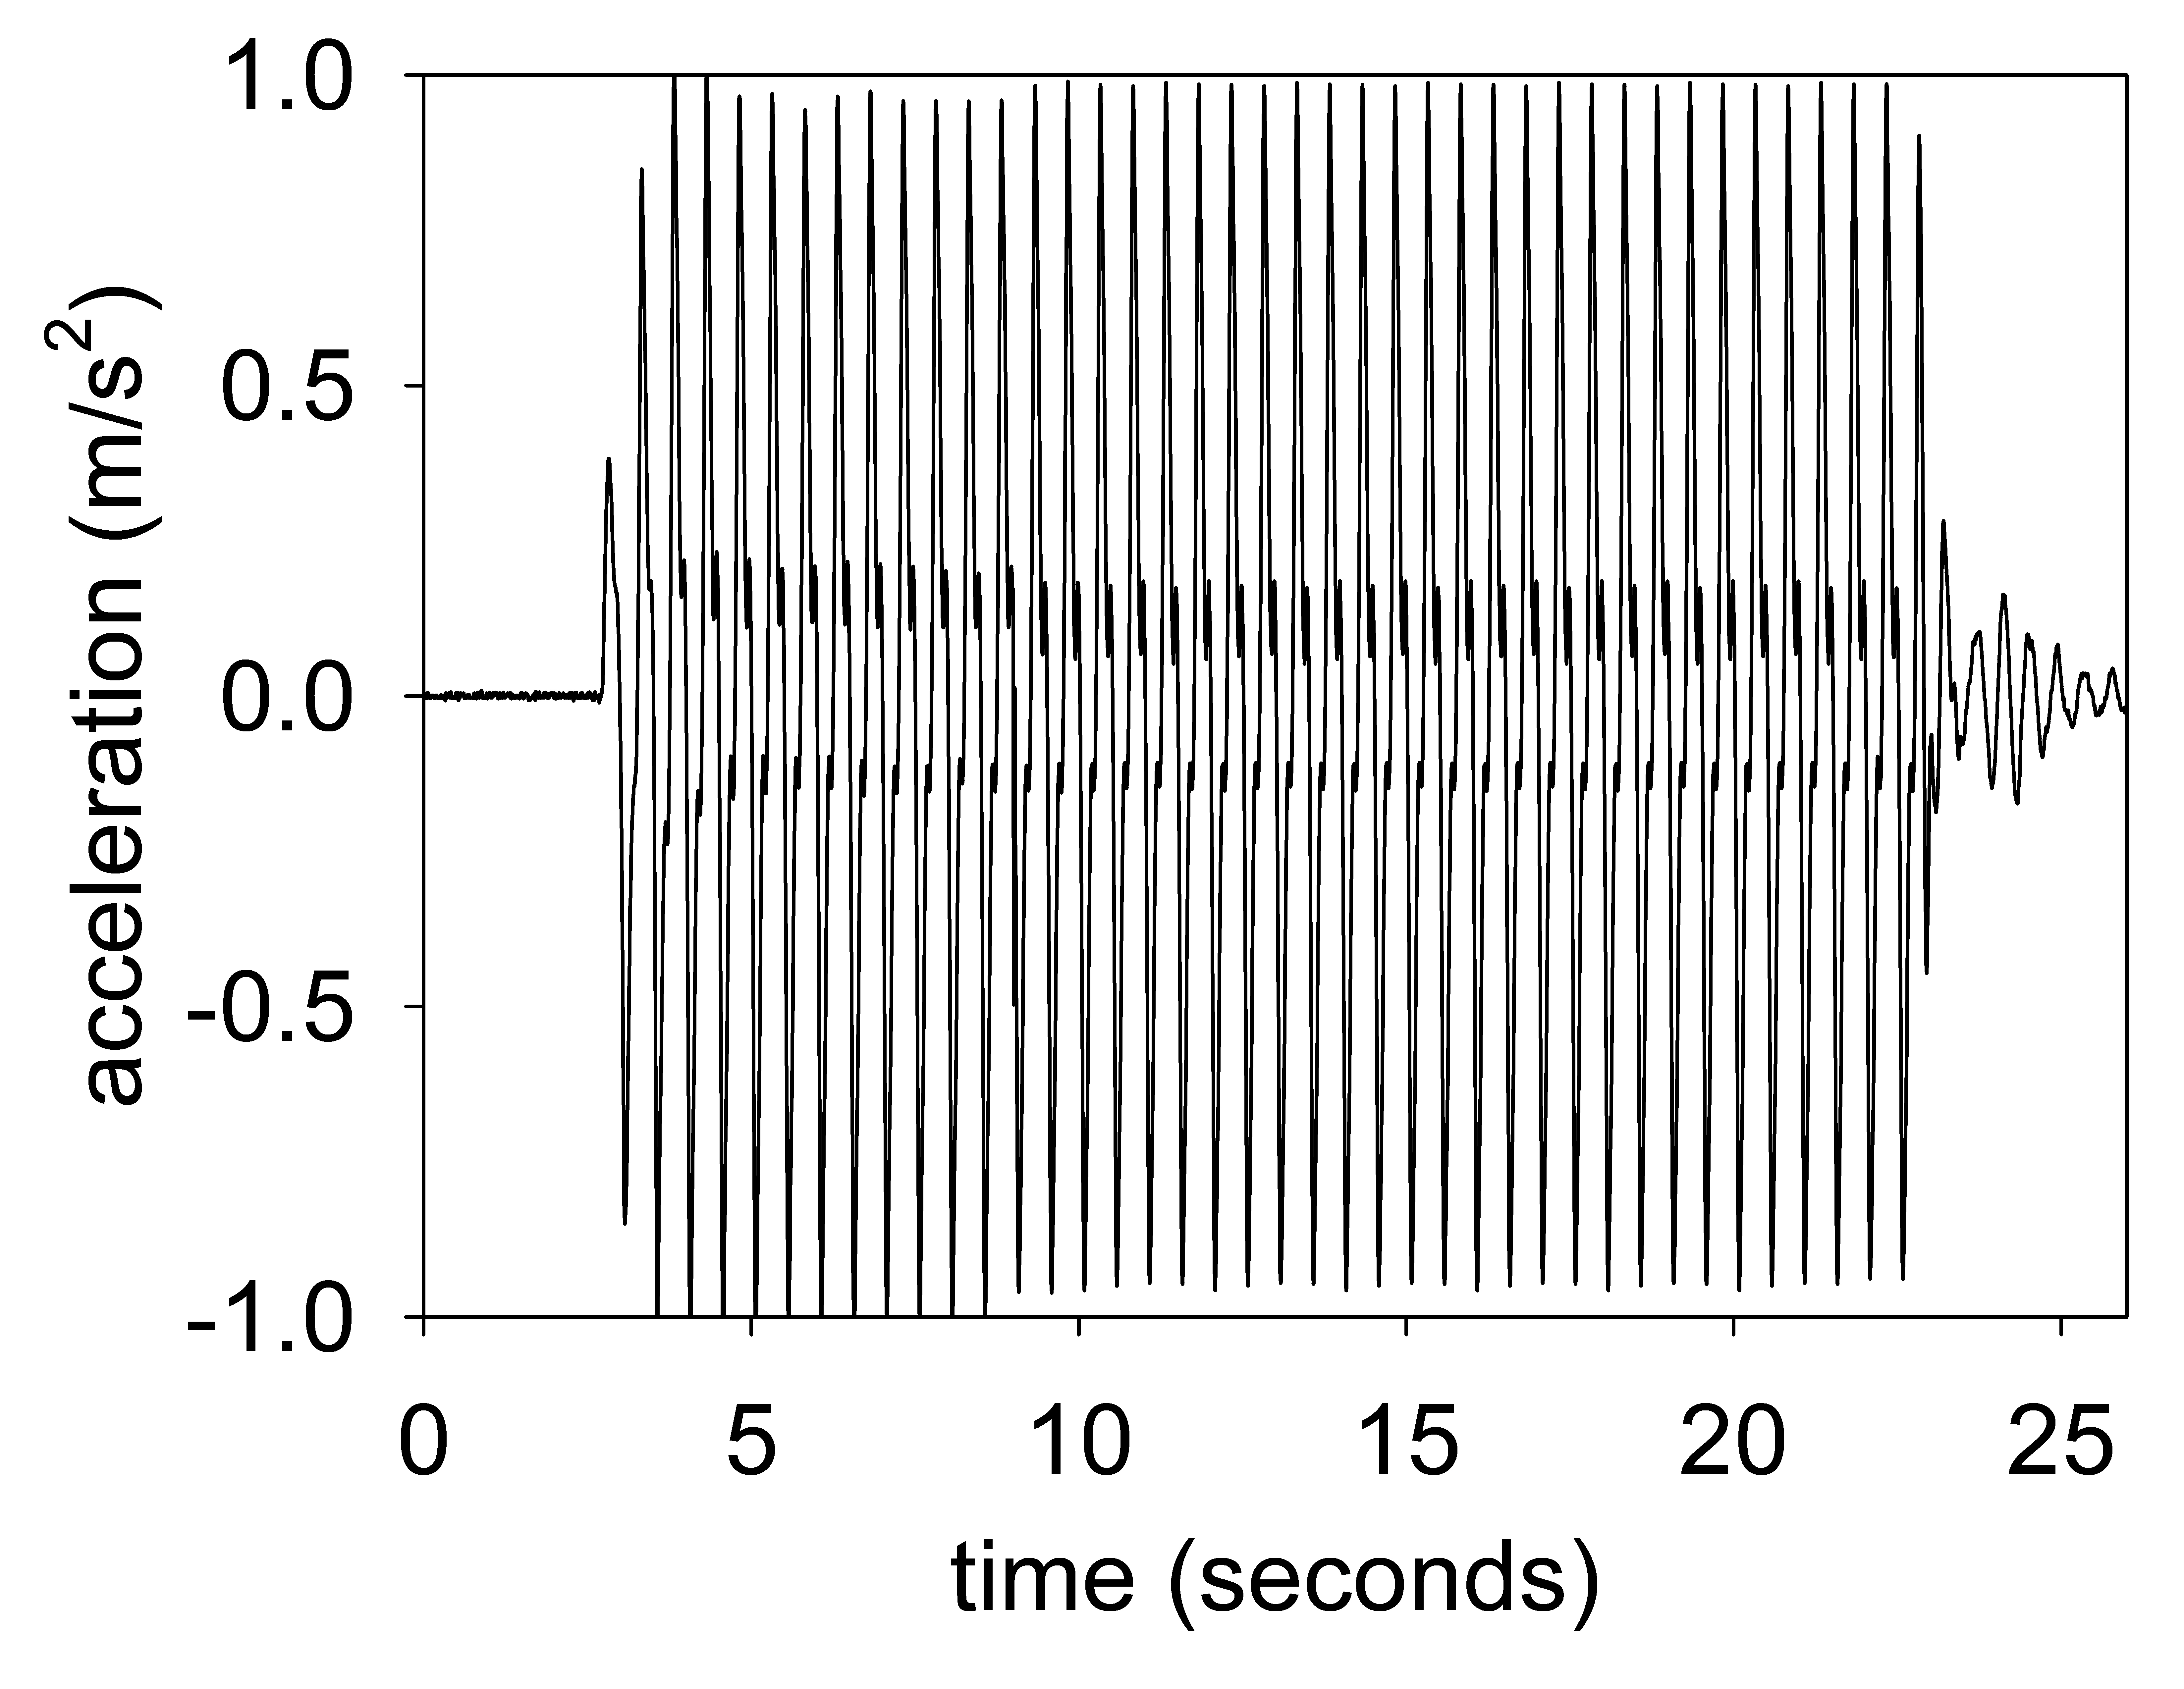
\includegraphics[width=\linewidth]{acer.jpg}
\caption{accerleration}
\end{subfigure}\hfill    
\begin{subfigure}[d]{0.5\linewidth}
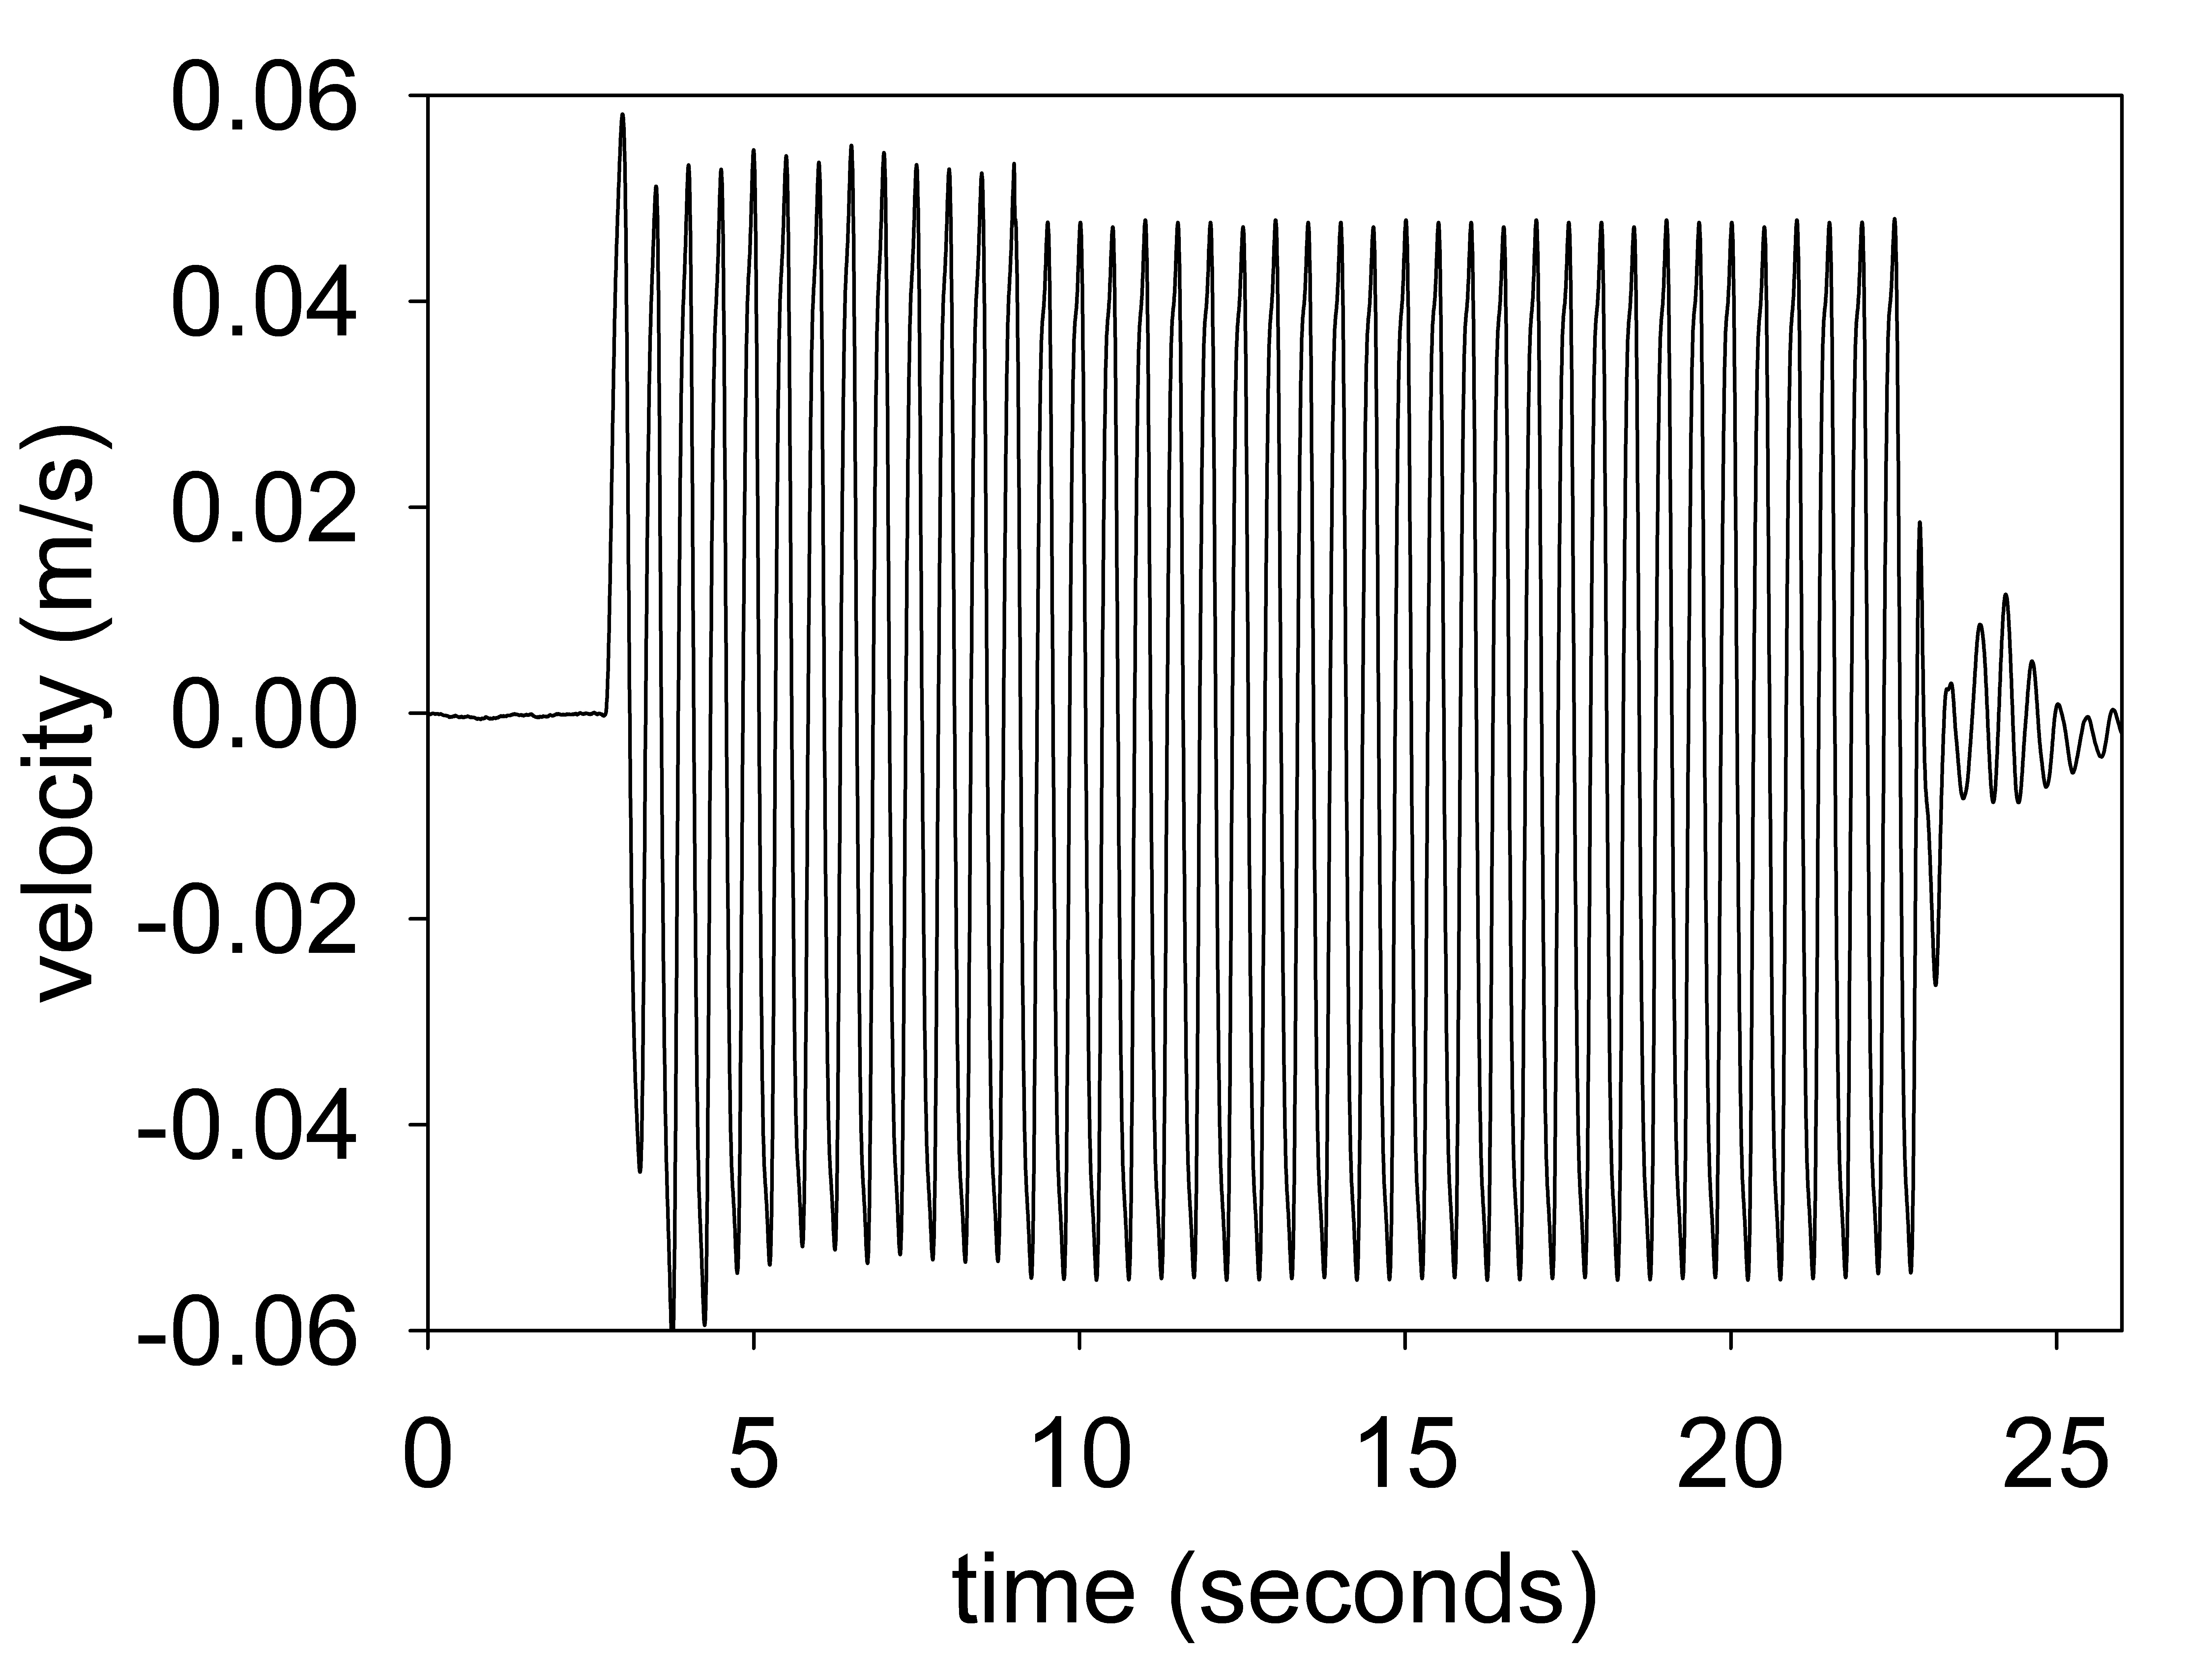
\includegraphics[width=\linewidth]{vel.jpg}
\caption{velocity}
\label{velocity}
\end{subfigure}
\caption{Ground acceleration profile, frequency of 2Hz and magnitude of 1g}
\label{groundacceleration}
\end{figure}
%
%
\begin{figure}[h]
\center
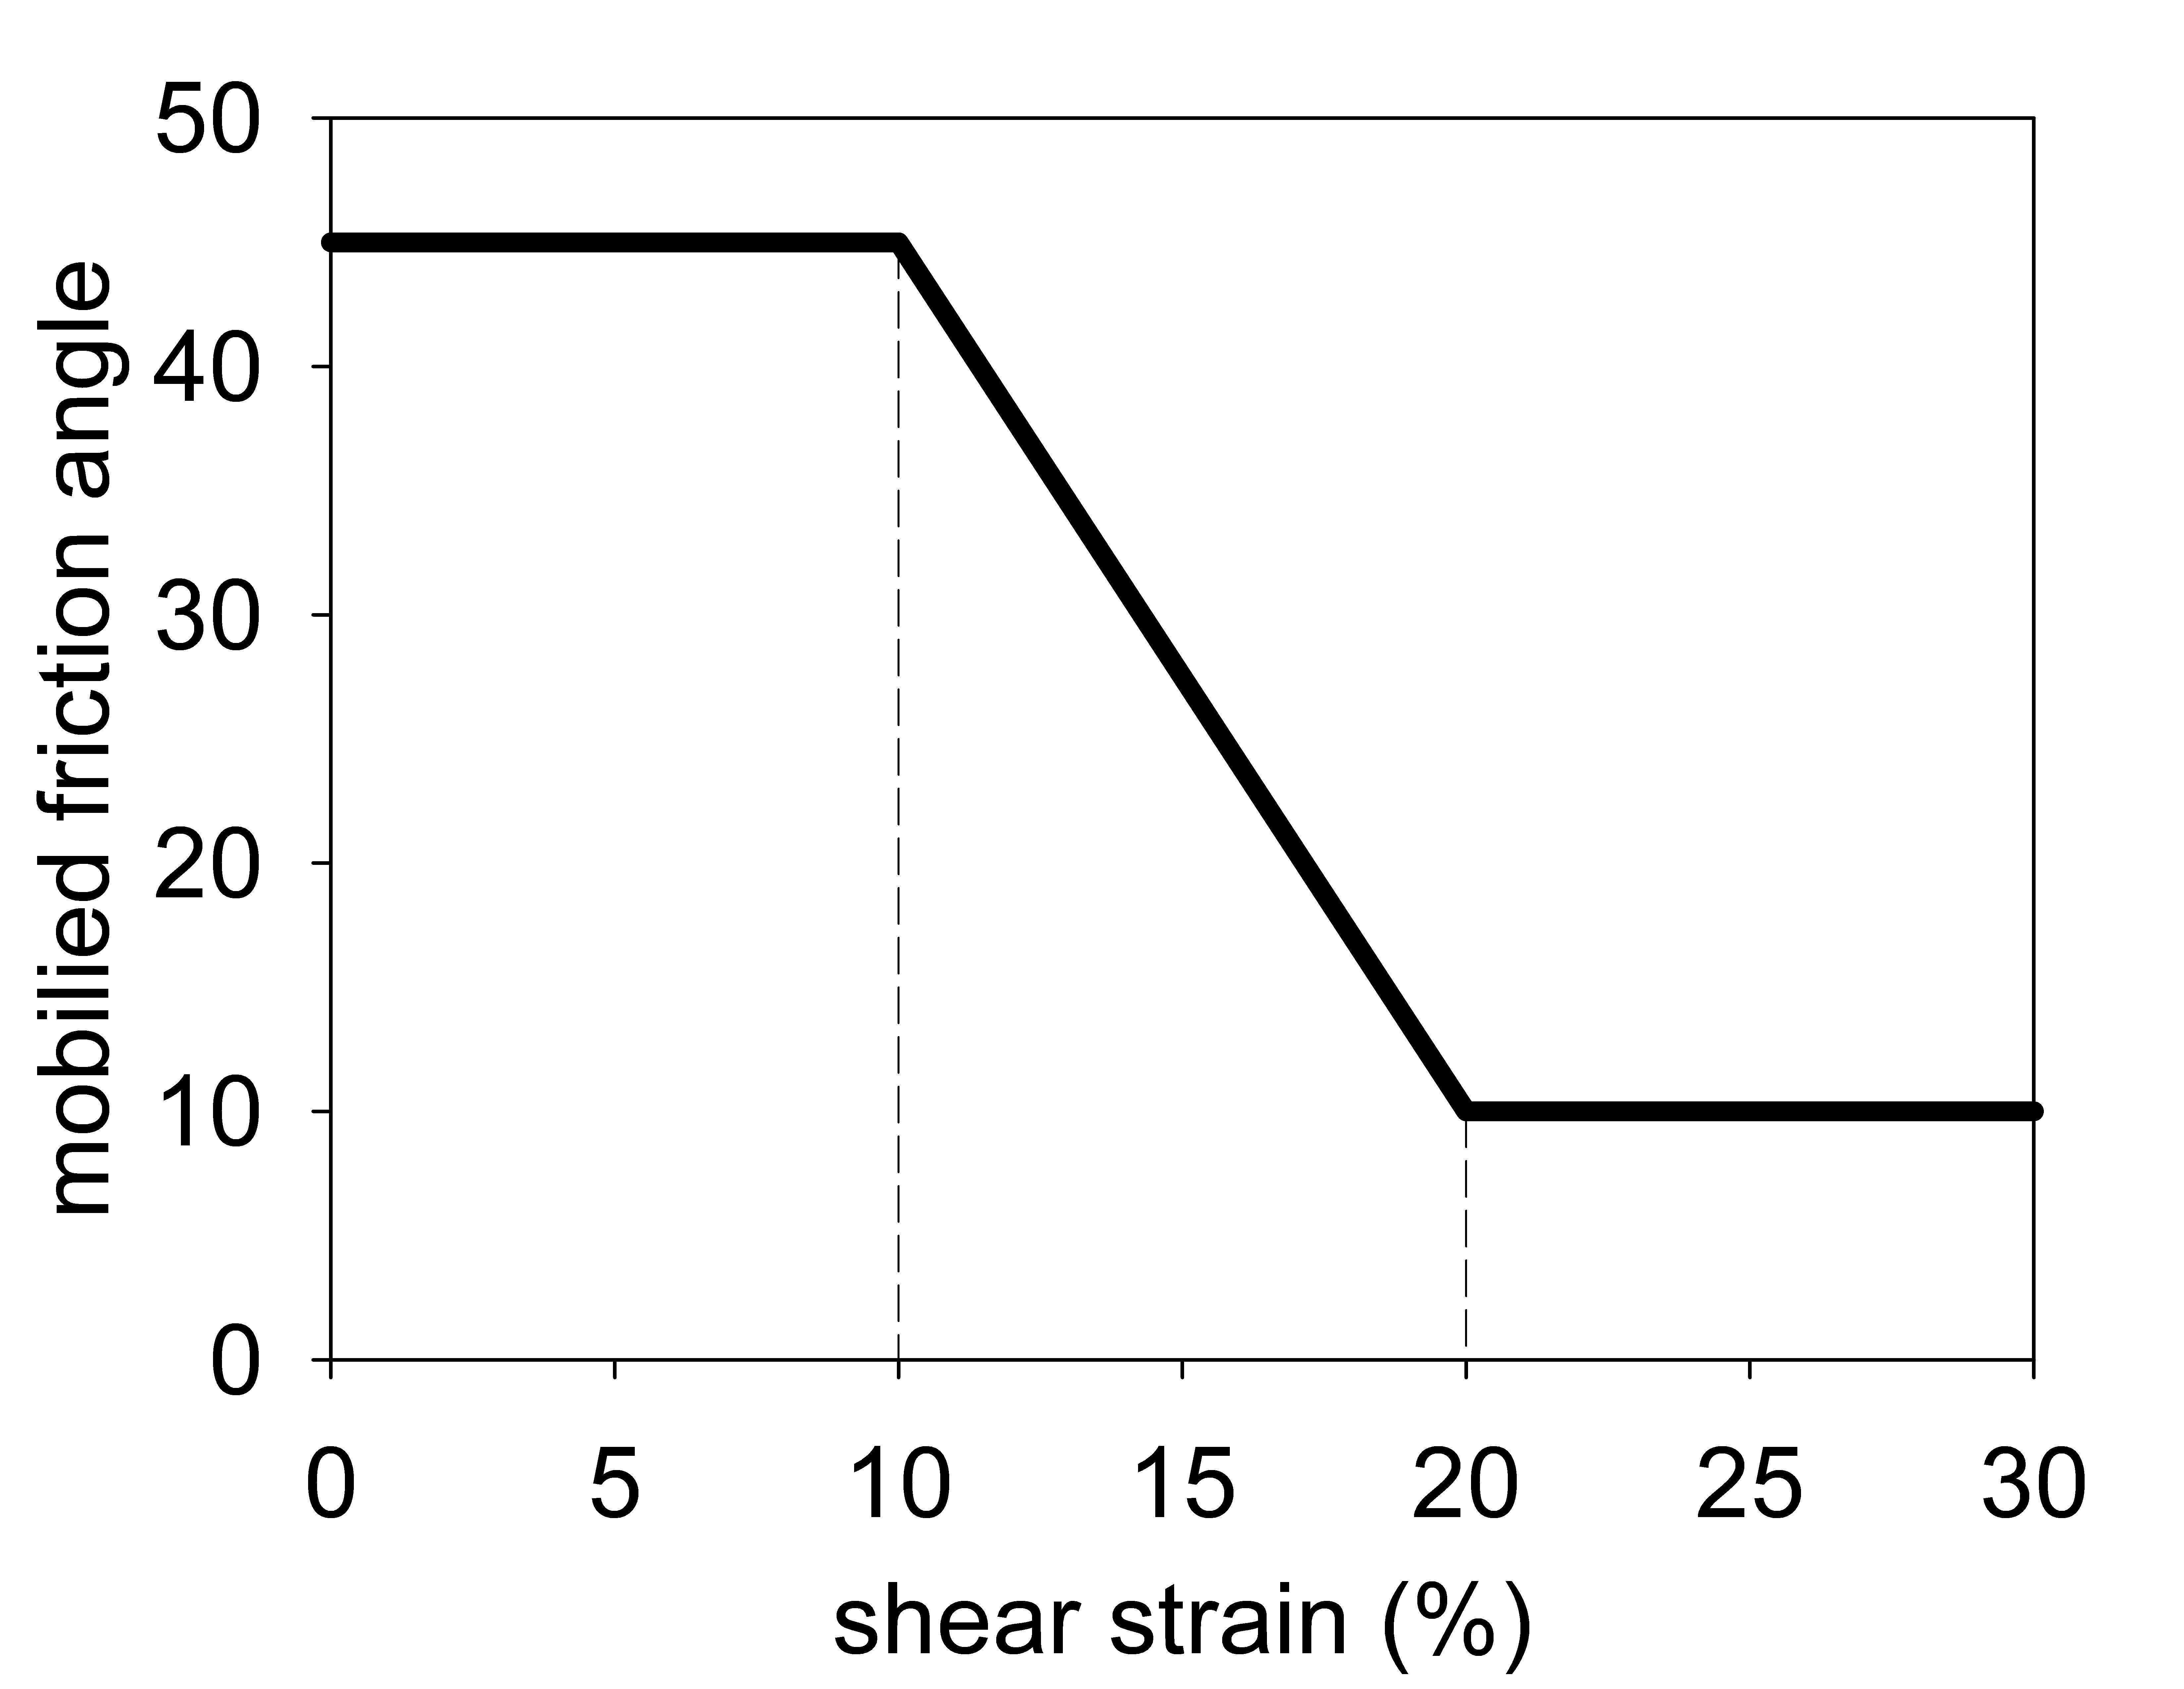
\includegraphics[scale=0.25]{model.jpg}
\caption{Mobilized friction angle in Mohr Coulomb model}
\label{fig:model}
\end{figure}
%
%
In the final example, we perform numerical analysis of the earthquake induced submarine landslides. We simplify the earthquake loading by simulating the ground shaking for 20 seconds with the peak ground acceleration of 1g and the frequency of 2Hz (see Figure \ref{groundacceleration}). The earthquake of this magnitude can occured typically for the earthquake of magnitude of more than 6. 
%
\begin{figure}[h]
\center
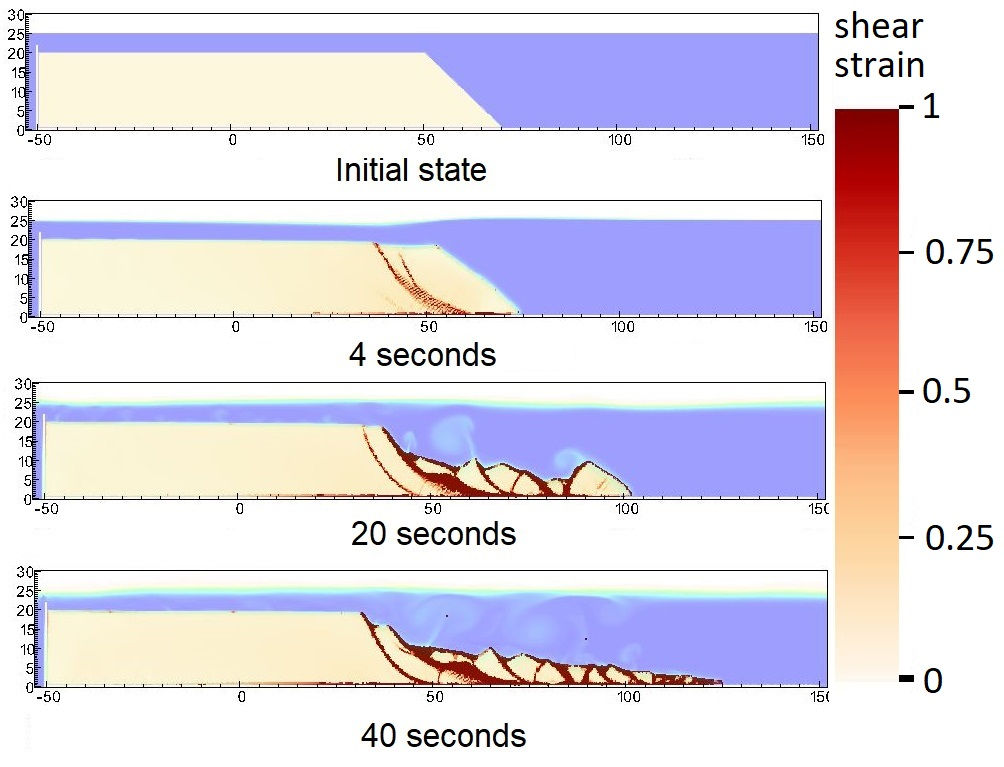
\includegraphics[scale=0.5]{landslide_gamma.jpeg}
\caption{Shear strain during the earthquake-induced submarine landslides}
\label{fig:gamma}
\end{figure}
%
%

%
%
\begin{figure}[h]
\center
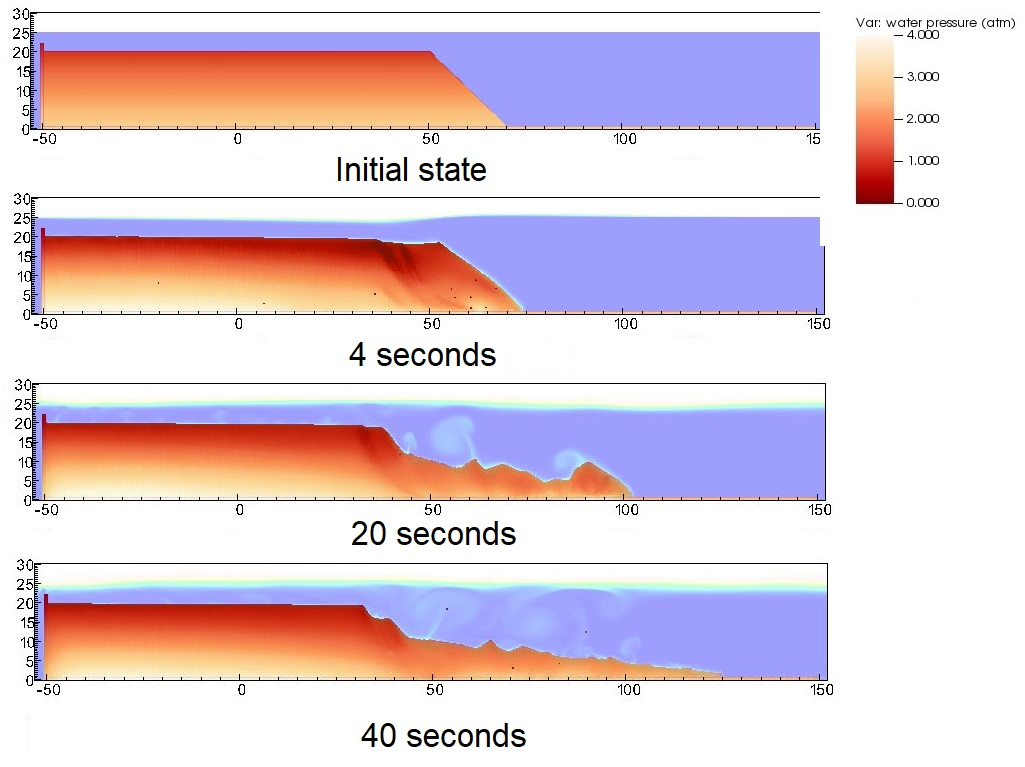
\includegraphics[scale=0.5]{PWP.jpeg}
\caption{pore water pressure during the earthquake-induced submarine landslides}
\label{fig:PWP}
\end{figure}
%
%

%
%
\begin{figure}[h]
\center
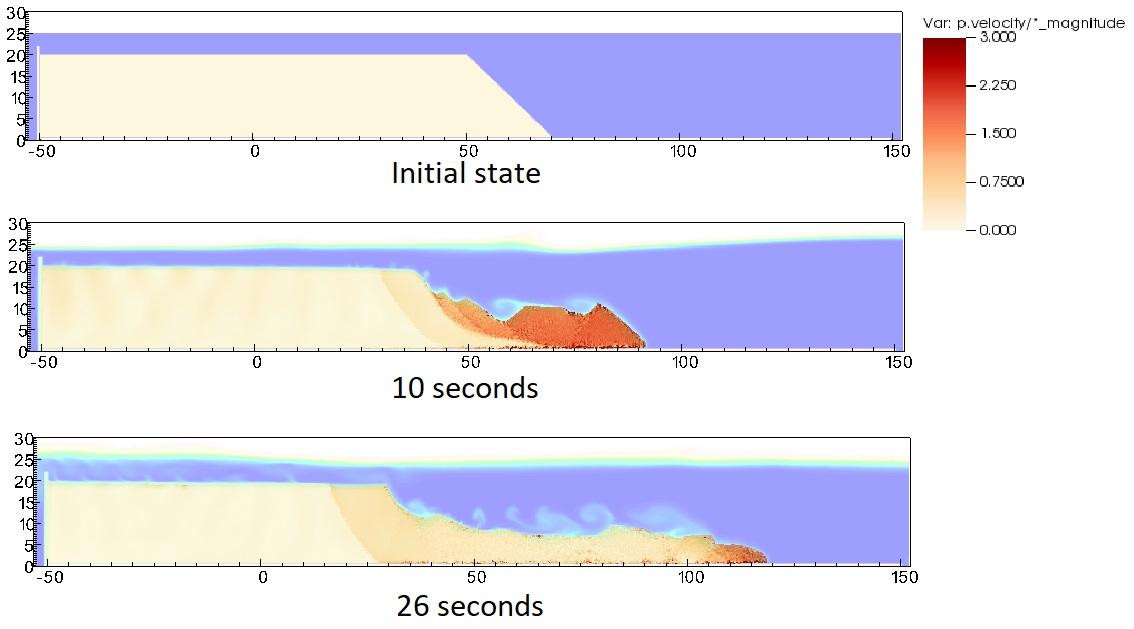
\includegraphics[scale=0.5]{landslide_vel.jpg}
\caption{Velocity during the earthquake-induced submarine landslides}
\label{fig:vel}
\end{figure}
%
%


%_______________________________
\section{\textsf{Conclusions}}

%_______________________________
\section{\textsf{Acknowledgements}}
The authors gratefully acknowledge Dr. James Guilkey and Dr. Todd Harman from the University of Utah for sharing the insight on the theoretical framework of MPMICE which this work is based. This project has received funding from the European Union’s Horizon 2020 research and innovation program under the Marie Skłodowska-Curie Actions (MSCA) Individual Fellowship (Project SUBSLIDE “Submarine landslides and their impacts on offshore infrastructures”) grant agreement 101022007. The authors would also like to acknowledge the support from the Research Council of Norway through its Centers of Excellence funding scheme, project number 262644 Porelab. The computations were performed on High Performance Computing resources provided by UNINETT Sigma2 - the National Infrastructure for High Performance Computing and Data Storage in Norway.

%_______________________________
%\appendix

\section{\textsf{Appendix}}
%
%
Before deriving the governing equation, we give some definition (following \cite{Kashiwa}) as below:
%
%
\begin{gather}
-\frac{1}{V} \left[ \frac{\partial V}{\partial p} \right] \equiv \kappa_f \qquad \mbox{ isothermal compressibility of fluid} \\
\frac{1}{V} \left[ \frac{\partial V}{\partial T} \right] \equiv \alpha_f \qquad \mbox{ contant pressure thermal expansivity of fluid}
\end{gather}
%
%
Then, the rate of volume with incompressible solid grains are calculated as below:
%
%
\begin{equation}
\label{fluidvolumerate}
\begin{gathered}
   \frac{1}{V} \frac{D_f V}{Dt} = \frac{1}{V} \left( \left[ \frac{\partial V}{\partial p} \right] \frac{D_f p}{D t} + \left[ \frac{\partial V}{\partial T} \right] \frac{D_f T}{D t} \right) = \frac{1}{V} \left( -\kappa \frac{D_f p}{D t} + \alpha \frac{D_f T}{D t} \right) \\
   = -(-\nabla \cdot \pmb{U}_f + \alpha_f \frac{D_f T_f}{Dt}) + \alpha_f \frac{D_f T_f}{Dt} = \nabla \cdot \pmb{U}_f
\end{gathered}
\end{equation}
%
%
\begin{equation}
\label{solidvolumerate}
 \frac{1}{V} \frac{D_s V}{D t} = \nabla \cdot \pmb{U}_s
\end{equation}
%
%
It is also convenient to define the Lagrangian derivative for a state variable $f$ as:
%
%
\begin{equation}
\frac{D_f f}{Dt} =  \frac{\partial f}{\partial t} + \pmb{U_f} \cdot \nabla f \qquad
\frac{D_s f}{Dt} =  \frac{\partial f}{\partial t} + \pmb{U_s} \cdot \nabla f
\end{equation}
%
%
\subsection{\textsf{Evolution of porosity}}
%
%
Solving the solid mass balance equation (\ref{massbalance}) with the definition of solid mass in equation (\ref{mass}), it leads to the rate of porosity as below:
%
%
\begin{equation}
   \frac{D_sm_s}{Dt} = \frac{D_s((1-n) \rho_s V)}{Dt} = \rho_s V \frac{D_s(1-n)}{Dt} + (1-n) V \frac{D_s \rho_s}{Dt} + (1-n) \rho_s  \frac{D_s V}{Dt} = 0  
\end{equation}
%
%
The soil grains are assumed to be incompressible, therefore, term 2 in the right hand side is zero. 
%
%
\begin{equation}
  V \frac{D_s(1-n)}{Dt} + (1-n) \frac{D_s V}{Dt} = 0  
\end{equation}
%
%
Dividing all terms with $V$ with the equation (\ref{fluidvolumerate}), it leads to:
%
%
\begin{equation}
  \frac{D_s n}{Dt} = \frac{\partial n}{\partial t} + \pmb{U}_s \cdot \nabla n = 
  (1-n) \nabla \cdot \pmb{U}_s  
\end{equation}
%
%
Finally, we get:
%
%
\begin{equation}
\label{p1}
\frac{\partial n}{\partial t} = (1-n) \nabla \cdot \pmb{U}_s  - \pmb{U}_s \cdot \nabla n
\end{equation}
%
%
\subsection{\textsf{Evolution of specific volume}}
%
%
The restriction for the equilibrium pressure can be derived from:
%
%
\begin{equation}
\begin{gathered}
    0 = \frac{\partial }{\partial t} (n - \sum_{f=1}^{N_f} \upsilon_f \rho_f) =  \frac{\partial n}{\partial t} - \sum_{f=1}^{N_f} (\rho_f\frac{\partial \upsilon_f}{\partial t} + \upsilon_f \frac{\partial \rho_f}{\partial t}) \\
= \frac{\partial n}{\partial t} - \sum_{f=1}^{N_f} (\rho_f\frac{D_f \upsilon_f}{Dt} + \nabla \cdot (\upsilon_f \rho_f \pmb{U}_f))\\
\label{equilP}
\end{gathered}
\end{equation}
%
%
Since the equation of sate shows that:
%
%
\begin{equation}
    \frac{D_f \upsilon_f}{Dt} = \upsilon_f (\kappa_f \frac{D_f P_{eq}}{Dt} + \alpha_f  \frac{D_f T_f}{Dt})
\label{specificvolume}
\end{equation}
%
%
Then equation (\ref{equilP}) becomes:
%
%
\begin{equation} 
\label{equilP1}
    0= \frac{\partial n}{\partial t} - \sum_{f=1}^{N_f} (\rho_f \upsilon_f (\kappa_f \frac{D_f P_{eq}}{Dt} + \alpha_f  \frac{D_f T_f}{Dt}) + \nabla \cdot (\upsilon_f \rho_f \pmb{U}_f))\\
\end{equation}
%
%
Putting equation (\ref{p1}) into equation (\ref{equilP1}) leads to:
%
%
\begin{equation} 
    \sum_{f=1}^{N_f}  \phi_f \kappa_f \frac{D_f P_{eq}}{Dt} = - \nabla \cdot \pmb{U} + \sum_{f=1}^{N_f} \phi_f \alpha_f \frac{D_f T_f}{Dt}
   \label{DP}
\end{equation}
%
%
where $\pmb{U} = \nabla \cdot (\sum_{s=1}^{N_s} \phi_s \pmb{U}_s + \sum_{f=1}^{N_f}  \phi_f \pmb{U}_f)$. And the rate of the specific volumne is computed by putting equation (\ref{DP}) into equation (\ref{specificvolume}):
\begin{equation}
\overline{\rho}_f \frac{D_f \upsilon_f }{Dt} = f_f^{\phi} \nabla \cdot \pmb{U} + (\phi_f \alpha_f \frac{D_f T_f}{Dt} - f_f^{\phi} \sum_{n=1}^{N} \phi_n \alpha_n \frac{D_n T_n}{Dt})
\end{equation}
where $ f_f^{\phi} = (\phi_f  \kappa_f ) / (\sum_{n=1}^{N} \phi_n \kappa_n)$ with  $\kappa_f$ being f-material bulk compressibility.
\subsection{\textsf{Momentum conservation}}
\label{Momentum}
%
%
The linear momentum balance equation for the fluid phase based on mixture theory is:\\
%
%
\begin{equation}
    \frac{1}{V}\frac{D_f(m_f \pmb{U}_f)}{Dt} = 
    \nabla \cdot (-np_f\pmb{I}) + \nabla \cdot \pmb{\tau}_f + \overline{\rho}_f \pmb{b} + \pmb{f}_{d} + \pmb{f}_b
\end{equation}
%
%
On the right hand sand, the first term is the divergence of partial fluid phase stress, the second term is the body force, the third term is the drag force (momentum exchange) and the fourth term is the buoyant force described in \cite{DRUMHELLER} for the immiscible mixtures. The buoyant force is in the form:\\
%
%
\begin{equation}
    \pmb{f}_b = \pmb{\sigma}_f\nabla (n)
\end{equation}
%
%
As a result, the linear momentum balance equation for fluid phase becomes:
%
%
\begin{equation}
    \label{fluidmom}
     \frac{1}{V}\frac{D_f(m_f \pmb{U}_f)}{Dt} = -n\nabla p_f + \nabla \cdot \pmb{\tau}_f + 
   \overline{\rho}_f \pmb{b} +
     \pmb{f}_{d}
\end{equation}
%
%
The Reynolds stress component can be included in the term $\pmb{\tau}_f$ to consider the turbulent effects if needed. To derive the linear momentum balance equation for the solid phase, we begin with the linear momentum balance equation for the mixture as:
%
%
\begin{equation}
    \label{totalmom}
     \frac{1}{V}\frac{D_f(m_f \pmb{U}_f)}{Dt}
    +  \frac{1}{V}\frac{D_s(m_s \pmb{U}_s)}{Dt} = 
    \nabla \cdot (\pmb{\sigma}) + \overline{\rho}_f \pmb{b} 
    + \overline{\rho}_s \pmb{b}
\end{equation}
%
%
Combining Terzaghi's equation (\ref{Terzaghi}) and subtracting both sides with equation (\ref{fluidmom}), we obtain the linear momentum balance equation for the solid phase as:
%
%
\begin{equation}
    \label{solidmom}
%     \frac{1}{V}\frac{D_s(m_s \pmb{U}_s)}{Dt} = 
    \nabla \cdot (\pmb{\sigma}^\prime) - (1-n) \nabla p_f 
    + \overline{\rho}_s \pmb{b}
    - \pmb{f}_{d}
\end{equation}
%
%
\subsection{\textsf{Energy conservation}}
We adopt the general form of the total energy balance equation for the porous media from \cite{Hassanizadeh}, the total energy balance equation for the fluid phase is:
%
%
\begin{equation}
\label{e1}
     \frac{1}{V}\frac{D_f(m_f (e_f+0.5\pmb{U}_f^2))}{Dt} = \nabla \cdot (-np_f\pmb{I}) \cdot \pmb{U}_f + \nabla \cdot \pmb{q}_f + (\overline{\rho}_f \pmb{b}) \cdot \pmb{U}_f + \pmb{f}_{d} \cdot \pmb{U}_f + q_{sf}
\end{equation}
%
%
Applying the product rule $D(m\pmb{U}^2)=D(m \pmb{U} \cdot \pmb{U}) = 2 \pmb{U} \cdot D(m \pmb{U})$, the left hand side of equation (\ref{e1}) becomes:\\
%
%
\begin{equation}
\label{e2}
     \frac{1}{V}\frac{D_f(m_f (e_f+0.5\pmb{U}_f^2))}{Dt} = \frac{1}{V}\frac{D_f(m_f e_f)}{Dt} + \frac{1}{V}\frac{D_f(m_f \pmb{U}_f)}{Dt} \cdot \pmb{U}_f 
\end{equation}
%
%
Combining equations (\ref{fluidmom}), (\ref{e1}), (\ref{e2}), we obtain the final form of the internal energy balance equation for the fluid phase as:
%
%
\begin{equation}
     \frac{1}{V}\frac{D_f(m_f e_f)}{Dt} = 
    -\overline{\rho}_f p  \frac{D_f\upsilon_f}{Dt} + \nabla \cdot \pmb{q}_f + q_{sf}
\end{equation}
%
%
On the right hand side, the terms include the average pressure-volume work, the average viscous dissipation, the thermal transport and the energy exchange between solid and fluid respectively. The heat flux is $\pmb{q}_f = \overline{\rho}_f \alpha_f \nabla T_f$. To derive the internal energy balance equation for the solid phase, we begin with the total energy balance equation for the mixture based on \cite{Hassanizadeh} as:\\
%
%
\begin{equation}
\label{e3}
\begin{gathered}
     \frac{1}{V}\frac{D_f(m_f (e_f+0.5\pmb{U}_f^2))}{Dt} + \frac{1}{V}\frac{D_s(m_s (e_s+0.5\pmb{U}_s^2))}{Dt} = \nabla \cdot (-np_f\pmb{I}) \cdot \pmb{U}_f \\
     + \nabla \cdot (\pmb{\sigma}^\prime-(1-n)p_f\pmb{I}) \cdot \pmb{U}_s + (-np_f\pmb{I}) : \nabla \pmb{U}_f + (\pmb{\sigma}^\prime-(1-n)p_f\pmb{I}) : \nabla \pmb{U}_s \\
     + (\overline{\rho}_f \pmb{b}) \cdot \pmb{U}_f + (\overline{\rho}_s \pmb{b}) \cdot \pmb{U}_s
     + \nabla \cdot \pmb{q}_f + \nabla \cdot \pmb{q}_s + \pmb{f}_{d} \cdot (\pmb{U}_f - \pmb{U}_s)  
\end{gathered}
\end{equation}
%
%
Subtracting equation (\ref{e3}) to equations (\ref{e1}) and (\ref{solidmom}), we obtained the internal energy balance equation for solid phase as:
%
%
\begin{equation}
     \frac{1}{V}\frac{D_s(m_s e_s)}{Dt} = \pmb{\sigma}^\prime:\nabla \pmb{U}_s
    + \nabla \cdot \pmb{q}_s - q_{sf} 
\end{equation}
%
%
On the right hand side, he terms include the mechanical work, thermal transport and energy exchange between solid and fluid respectively. The heat flux is $\pmb{q}_s = \overline{\rho}_s \alpha_s \nabla T_s$
%
%
\subsection{\textsf{Advanced Fluid Pressure}}
The discretization of the pressure equation begins with the Lagrangian face-centered velocity and the equation for the pressure
%
\begin{equation}
 \label{append:pressure1}
  \overline{\rho}_{f,FC} \frac{\pmb{U}_{f,FC}^{n+1} - \pmb{U}_{f,FC}^{n}}{dt} 
  = n \nabla^{FC} P_{fc}^{n+1} + \overline{\rho}_{f,FC} \pmb{b}
\end{equation}
%
%
\begin{equation}
\label{append:pressure2}
  \kappa \frac{dP}{dt} = \nabla^c \cdot \pmb{U}_{f,FC}^{n+1}
\end{equation}
%
The divergence of the equation (\ref{append:pressure1}) with $ \nabla \cdot \pmb{b} = 0$ is
%
\begin{equation}
\label{append:pressure3}
  \nabla^c \cdot \pmb{U}_{f,FC}^{n+1} - \nabla^c \cdot \pmb{U}_{f,FC}^{n}
  = \nabla^c \frac{\delt}{\rho_{f,FC}^n} \cdot \nabla^{FC} (P_{fc}^{n} + \Delta P_{fc}^{n})
\end{equation}
%
To solve this equation, we define the face-centered intermediate velocity $ \pmb{U}_{f,FC}^{*}$ as:
%
\begin{equation}
 \label{append:pressure4}
  \overline{\rho}_{f,FC} \frac{\pmb{U}_{f,FC}^{*} - \pmb{U}_{f,FC}^{n}}{\delt} 
  = n \nabla^{FC} P_{fc}^{n} + \overline{\rho}_{f,FC} \pmb{b}
\end{equation}
%
%
The divergence of the equation (\ref{append:pressure4}) is
%
\begin{equation}
\label{append:pressure5}
  \nabla^c \cdot \pmb{U}_{f,FC}^{*} - \nabla^c \cdot \pmb{U}_{f,FC}^{n}
  = \nabla^c \frac{\delt}{\rho_{f,FC}^n} \cdot \nabla^{FC} P_{fc}^{n}
\end{equation}
%
Combining equations (\ref{append:pressure2}, \ref{append:pressure3}, \ref{append:pressure5}), it leads to
\begin{equation}
\label{append:pressure6}
  \left(  
   \kappa - \nabla^c \frac{\delt}{\rho_{f,FC}^n} \cdot \nabla^{FC}
  \right) \Delta P_{fc}^{n} = - \nabla^c \cdot \pmb{U}_{f,FC}^{*}
\end{equation}
When the fluid is incompressible, $\kappa$ approaches to zero and the equation (\ref{append:pressure6}) becomes the Poisson's equation for the incompressible fluid flow.
%
%
\subsection{\textsf{Momentum exchange with an implicit solve}}
%
%
Considering the fluid momentum balance equation as 
%
\begin{equation}
  (m\pmb{U})_{f,FC}^{n+1} =  (m\pmb{U})_{f,FC}^{n} - \delt (V n \nabla^{FC} P_{fc}^{n} + m_f \pmb{b}) + V K \delt (\pmb{U}_{s,FC}^{n+1} - \pmb{U}_{f,FC}^{n+1})
\end{equation}
%
%
Assuming $m_{f,FC}^{n+1} = m_{f,FC}^n$ we get
%
\begin{equation}
  \pmb{U}_{f,FC}^{n+1} =  \pmb{U}_{f,FC}^{n} - \delt (\frac{\nabla^{FC} P_{fc}^{n}} {\rho_{f,FC}^n} + \pmb{b}) + \frac{\delt K}{\overline{\rho}_{f,FC}^n} (\pmb{U}_{s,FC}^{n+1} - \pmb{U}_{f,FC}^{n+1})
\end{equation}
%
%
As defined in the section 'Advanced Fluid Pressure', the face-centered intermediate fluid velocity $\pmb{U}_{f,FC}^{*} = \delt (\nabla^{FC} P_{fc}^{n} / \rho_{f,FC}^n + \pmb{b})$ leading to
%
\begin{equation}
\label{append:exchange1}
  \pmb{U}_{f,FC}^{n+1} =  \pmb{U}_{f,FC}^{*} +  \frac{\delt K}{\overline{\rho}_{f,FC}^n} (\pmb{U}_{s,FC}^{n+1} - \pmb{U}_{f,FC}^{n+1})
\end{equation}
%
%
Considering the solid momentum balance equation as
%
\begin{equation}
  (m\pmb{U})_{s,FC}^{n+1} =  (m\pmb{U})_{s,FC}^{n} - \delt (V \nabla^{FC} \cdot \pmb{\sigma}^{'n} - V (1-n) \nabla^{FC} P_{fc}^{n} + m_s \pmb{b}) - V K \delt (\pmb{U}_{s,FC}^{n+1} - \pmb{U}_{f,FC}^{n+1})
\end{equation}
%
%
We define the face-centered intermediate solid velocity as $\pmb{U}_{s,FC}^{*} = \delt (\nabla^{FC} \cdot \pmb{\sigma}_c^{'n} / \overline{\rho}_{s,FC}  - \nabla^{FC} P_{fc}^{n} / \rho_s + \pmb{b})$ leading to
%
\begin{equation}
\label{append:exchange2}
  \pmb{U}_{s,FC}^{n+1} =  \pmb{U}_{s,FC}^{*} -  \frac{\delt K}{\overline{\rho}_{s,FC}^n} (\pmb{U}_{s,FC}^{n+1} - \pmb{U}_{f,FC}^{n+1})
\end{equation}
%
%
Combining equation (\ref{append:exchange1}) and (\ref{append:exchange2}) we get
%
\begin{equation}
\begin{gathered}
\label{append:exchange3}
  \pmb{U}_{f,FC}^{*} + \Delta \pmb{U}_{f,FC} =  \pmb{U}_{f,FC}^{*} +  \frac{\delt K}{\overline{\rho}_{f,FC}^n} (\pmb{U}_{s,FC}^{*} + \Delta \pmb{U}_{s,FC} - \pmb{U}_{f,FC}^{*} - \Delta \pmb{U}_{f,FC}) \\
  \pmb{U}_{s,FC}^{*} + \Delta \pmb{U}_{s,FC} =  \pmb{U}_{s,FC}^{*} -  \frac{\delt K}{\overline{\rho}_{s,FC}^n} (\pmb{U}_{s,FC}^{*} + \Delta \pmb{U}_{s,FC} - \pmb{U}_{f,FC}^{*} - \Delta \pmb{U}_{f,FC})
\end{gathered}
\end{equation}
%
%
Rearranging the equation (\ref{append:exchange3}), it leads to the linear system of equations
%
\[ \begin{vmatrix} (1 + \beta_{12,FC})  &  -\beta_{12,FC} \\
                  -\beta_{21,FC}       &  (1 + \beta_{21,FC})
    \end{vmatrix}
    \begin{vmatrix} \Delta \pmb{U}_{f,FC} \\
                    \Delta \pmb{U}_{s,FC}
    \end{vmatrix}
    =
    \begin{vmatrix}  \beta_{12,FC}(\pmb{U}_{s,FC}^{*} - \pmb{U}_{f,FC}^{*}) \\
                    \beta_{21,FC}(\pmb{U}_{f,FC}^{*} - \pmb{U}_{s,FC}^{*})
    \end{vmatrix}                
\]
%
%
Solving this linear equations with $\beta_{12,FC} = (\delt K)/\overline{\rho}_{f,FC}^n$ and $\beta_{21,FC} = (\delt K)/\overline{\rho}_{s,FC}^n$. Similar derivation can be performed to computed the cell-center velocity increment leading to
%
\[ \begin{vmatrix} (1 + \beta_{12c})  &  -\beta_{12c} \\
                  -\beta_{21c}       &  (1 + \beta_{21c})
    \end{vmatrix}
    \begin{vmatrix} \Delta \pmb{U}_{fc} \\
                    \Delta \pmb{U}_{sc}
    \end{vmatrix}
    =
    \begin{vmatrix}  \beta_{12c}(\pmb{U}_{sc}^{*} - \pmb{U}_{fc}^{*}) \\
                    \beta_{21c}(\pmb{U}_{fc}^{*} - \pmb{U}_{sc}^{*})
    \end{vmatrix}                
\]
%
%
with $\beta_{12c} = (\delt K)/\overline{\rho}_{fc}^n$ and $\beta_{21c} = (\delt K)/\overline{\rho}_{sc}^n$ and the cell-centered intermediate velocity can be calculated by
%
\begin{equation}
\begin{gathered}
\pmb{U}_{fc}^{*} = \pmb{U}_{fc}^{n} + \delt (-\frac{\nabla P_{fc}^{n+1}}{\rho_{fc}^n}  + \frac {\nabla \cdot \pmb{\tau}_{fc}^{n}}{\overline{\rho}^n_{fc}} + \pmb{b}) \\
\pmb{U}_{sc}^{*} = \pmb{U}_{sc}^{n} + \delt (\frac{\nabla \cdot \pmb{\sigma}_c^{'n}}{\overline{\rho}^n_{sc}}    - \frac{\nabla P_{fc}^{n+1}}{\rho_s}  + \pmb{b})
\end{gathered}
\end{equation}
%
%
%% The Appendices part is started with the command \appendix;
%% appendix sections are then done as normal sections
%% \appendix

%% \section{}
%% \label{}

%% If you have bibdatabase file and want bibtex to generate the
%% bibitems, please use
%%
%%\bibliographystyle{elsarticle-num} 
%%\bibliography{<MPMICE2>}

%% else use the following coding to input the bibitems directly in the
%% TeX file.

%% \begin{thebibliography}{00}
%% \bibitem{label}
%% Text of bibliographic item
%% \end{thebibliography}

\bibliography{MPMICE2}
\end{document}
\endinput
%%
%% End of file `elsarticle-template-num.tex'.
